\chapter{Vocabularies for Personal Datastores}
\label{chap:vocabularies}

\begin{tcolorbox}[colback=royallavender!40]
The content of this Chapter has already been partially included in the articles published during this Thesis \citep{esteves_odrl_2021,esteves_using_2023,esteves_fostering_2022}.
\end{tcolorbox}

\begin{tcolorbox}[colback=royallavender!10]
The source code produced during the development of this chapter is stored at:
\begin{itemize}
    \item \url{https://w3id.org/oac/repo}
    \item \url{https://w3id.org/oac/policies}
    \item \url{https://w3id.org/plasma/repo}
    \item \url{https://w3id.org/people/besteves/justifications/repo}
\end{itemize}
\end{tcolorbox}

This Chapter builds upon existing Semantic Web standards and specifications to develop a set of vocabularies that can support data subjects in the expression of their privacy preferences when it comes to accessing their data and exercising their rights, as well as data controllers to deal with their \textit{``[t]ransparent information''} requirements, explicitly set in GDPR's Articles 12--14.
As previously established in Section \ref{sec:sota_solid}, Solid's access control and interoperability specifications do not contain the terms to satisfy said requirements, and as such, the incorporation of these vocabularies will lead to a GDPR-aligned personal datastore.

Thus, Section \ref{sec:oac} describes the development of an ODRL profile (OAC) with the main goal of defining legally aligned policies that express permissions and/or prohibitions associated with purpose-based access to data stored in decentralised storage environments, such as Solid Pods.
Such policies will be used to express the data subjects' preferences concerning the access to their \textit{personal} data, to represent requests to access data, and to record the agreed access conditions for future inspection.

Section \ref{sec:plasma} describes the development of a metadata language for Solid (PLASMA) to provide consistent taxonomies to describe the entities, infrastructure, policies, notices, registries, and logs necessary to understand and establish responsibilities and accountability within the Solid ecosystem.
PLASMA utilises OAC to express data policies, provides a set of conformance conditions that should be met by Pod, app, and service providers, as well as users and agents, to comply with the established specification and a description of workflows where PLASMA terms should be used to satisfy such conformance conditions.

Section \ref{sec:rights_exercising} showcases the usage of vocabulary-based, e.g. DPV, DCMI, PROV-O, and DCAT, patterns to describe rights exercising metadata with the goal of providing uniform records of data subject rights exercising activities.

Section \ref{sec:evaluation} presents the results of the ontologies quality evaluation, including the detection of common pitfalls with OOPS!, alignment with FAIR principles with FOOPS! and validation of competency questions with SPARQL queries, and Section~\ref{sec:iso_27560} discusses the alignment with the ISO/IEC 27560 standard on `Consent record information structure'.

The methodology followed to develop and evaluate the vocabularies described in this Chapter is described in Section \ref{sec:ontology_engineering}.
The prefixes and namespaces used in the Listings in this Chapter are explicitly defined in the \hyperref[sec:namespaces]{Namespaces list}.

\section{Background}
\label{sec:background_vocabs}

As established through the state of the art and in the comparative analysis performed in Sections \ref{sec:sota_vocabularies_analysis} and \ref{sec:sota_policies_analysis}, DPV contains the highest number of concepts to model GDPR's rights and obligations and their privacy terms, is being actively developed and maintained, is open and accessible, and ODRL supports the modelling of deontic concepts, e.g., permissions or obligations, constraints, e.g., spatial and temporal, and types of policies, e.g., offers, requests and agreements, and has a mechanism to develop extensions to its vocabulary through profiles.
As such, they can be used as a starting point to express policies for access to personal data, while invoking privacy and data protection-specific terms.

Figure \ref{fig:odrl} presents a diagram of the ODRL Information Model.
Its main goal is to \textit{``enable flexible Policy expressions by allowing the policy author to include as much, or as little, detail in the Policies''} \citep{iannella_odrl_2018}, using the terms defined in the ODRL Vocabulary \& Expression specification \citep{iannella_odrl_vocab_2018}.
Table \ref{tab:odrl} provides an overview of the concepts modelled in the ODRL vocabulary.

\begin{figure}[htbp]
\caption{ODRL Information Model, adapted from \cite{iannella_odrl_2018}.}
\label{fig:odrl}
\centering
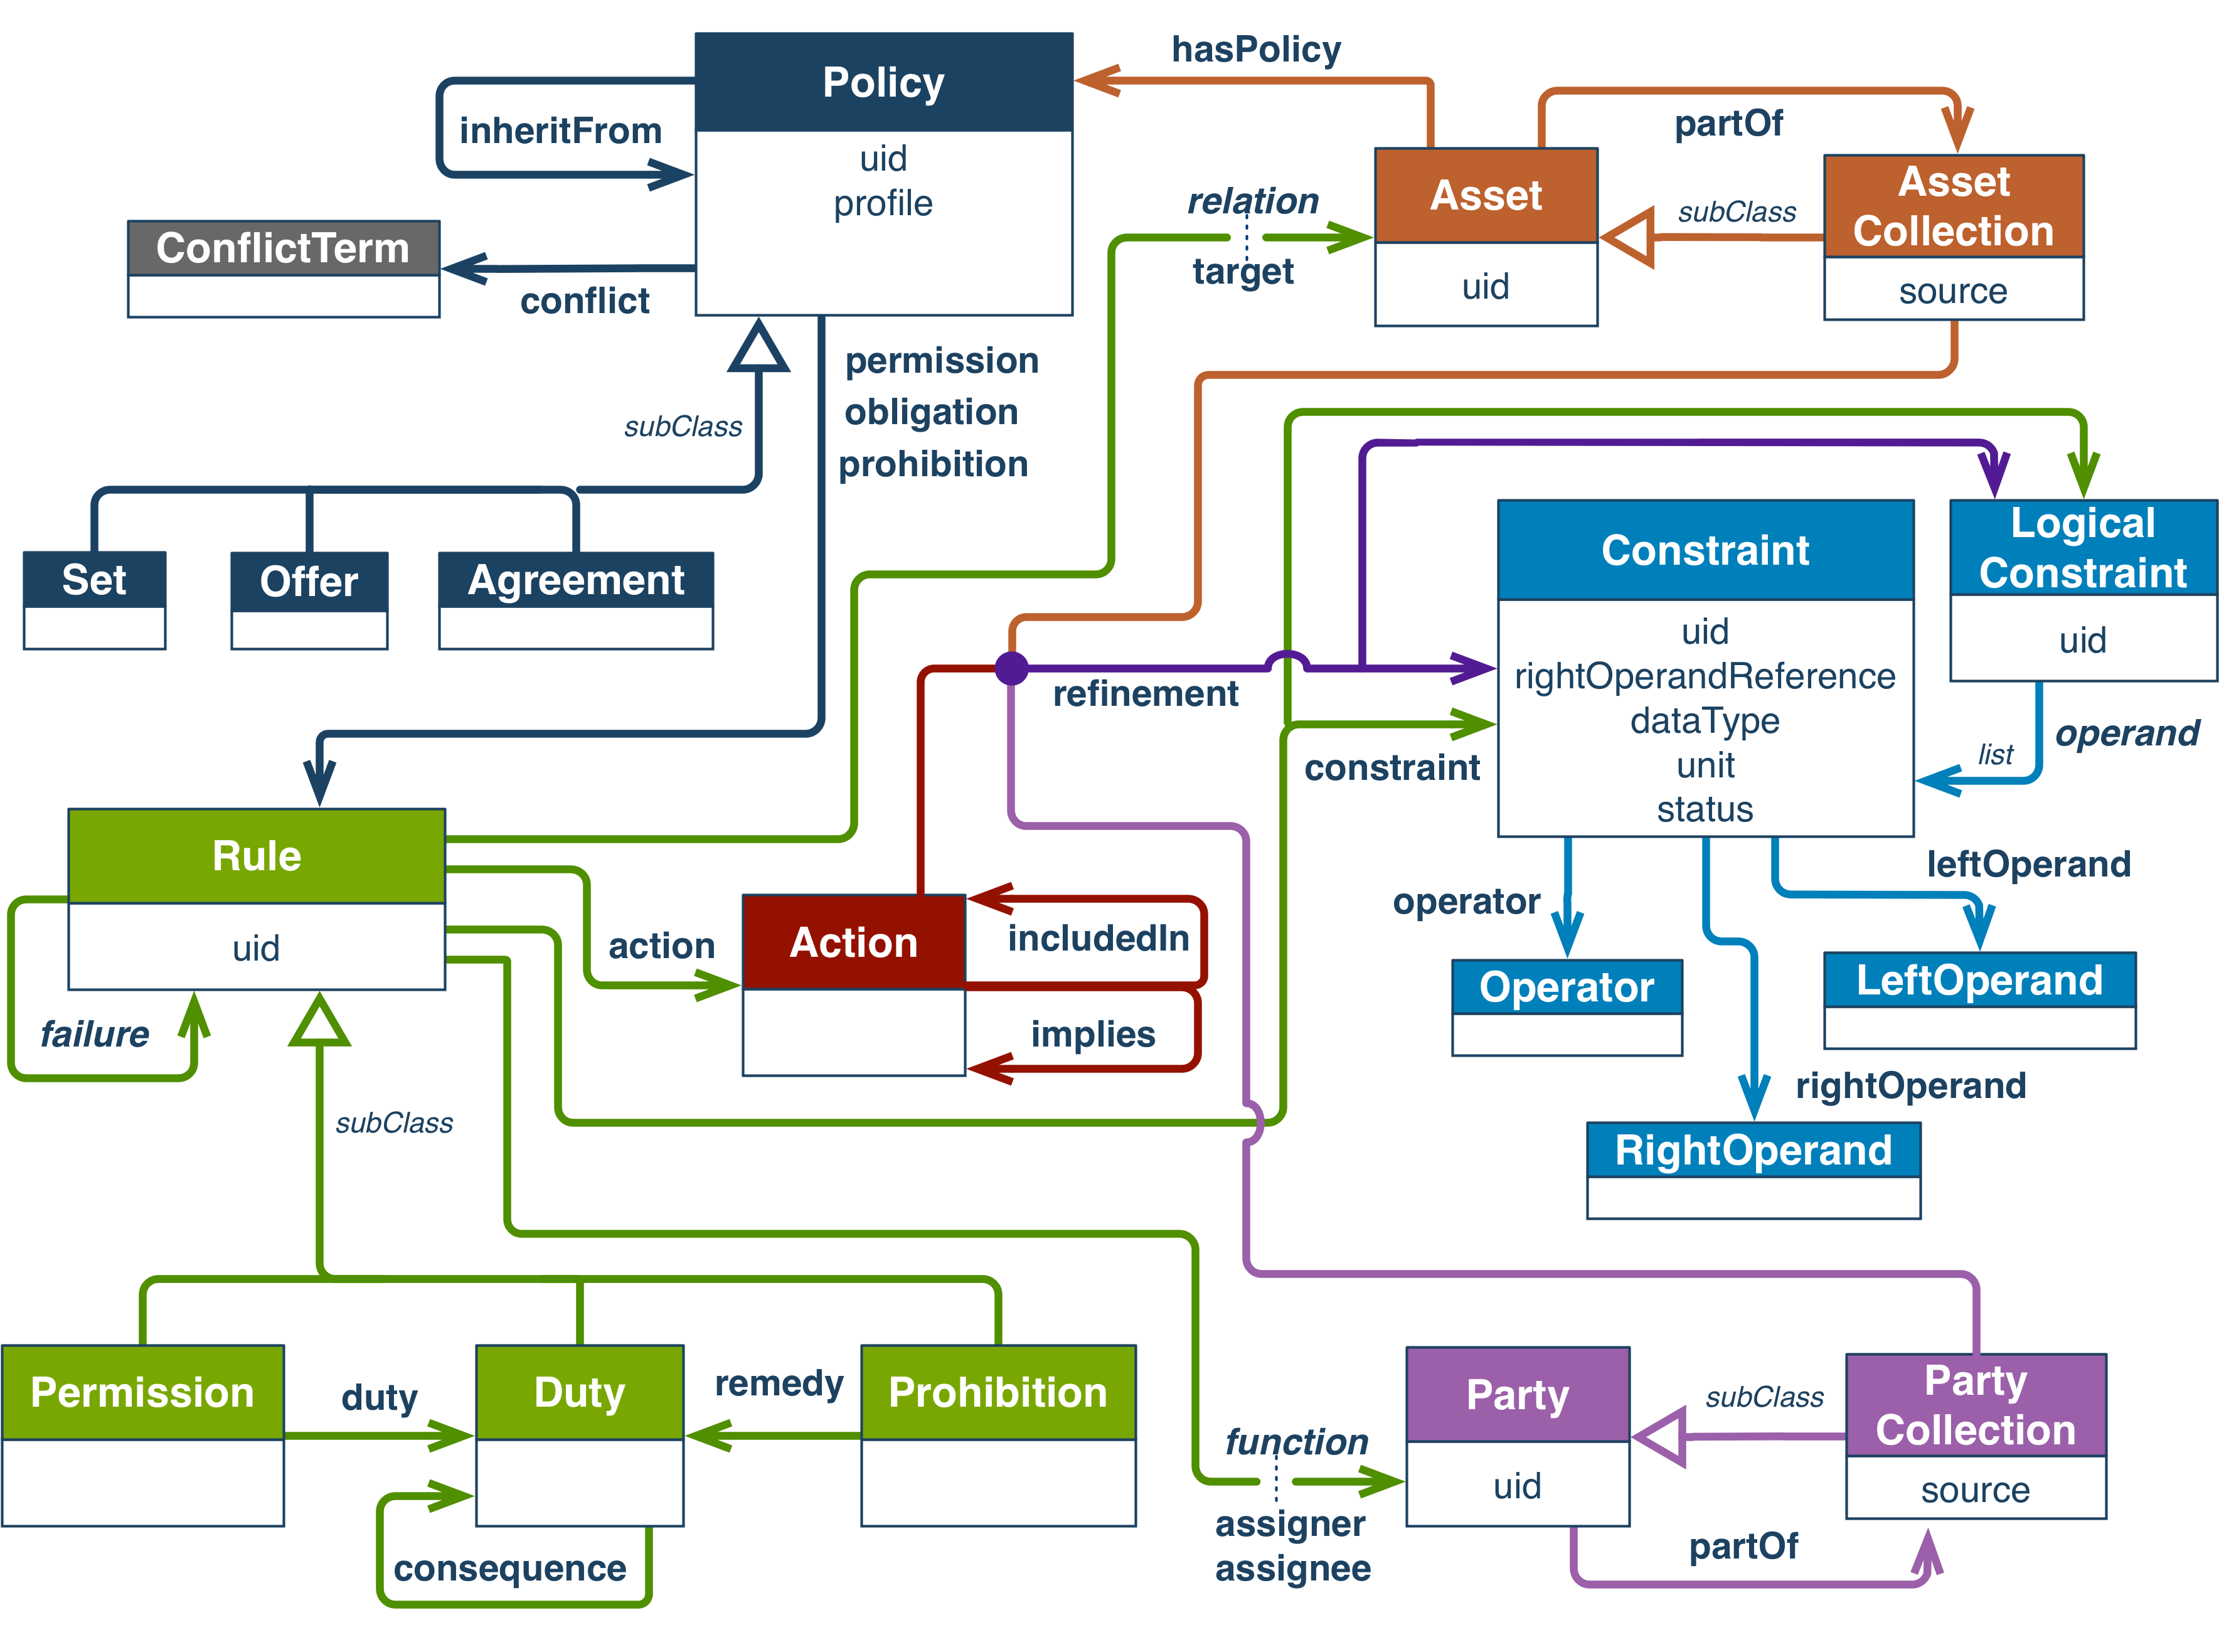
\includegraphics[width=0.8\textwidth]{figures/chapter-4/ODRL.png}
\end{figure}

\begin{table}[htbp]
\caption{Overview of the concepts modelled in the ODRL vocabulary.}
\label{tab:odrl}
\centering
\begin{tabular}{c||c}
Concept & Subclasses \\
\hline\hline
Policy & Agreement, Assertion, Offer, Privacy, Request, Set, Ticket \\
\hline
Rule & Duty, Permission, Prohibition\\
\hline
\begin{tabular}[c]{@{}c@{}}Party\\ functions\end{tabular} & \begin{tabular}[c]{@{}c@{}}assignee, assigner, attributedParty, attributingParty, \\ compensatedParty, compensatingParty, consentedParty, \\ consentingParty, contractedParty, contractingParty, informedParty, \\ informingParty, trackedParty, trackingParty\end{tabular}\\
\hline
Action & \begin{tabular}[c]{@{}c@{}}Attribution, CommericalUse, DerivativeWorks, Distribution, Notice, \\ Reproduction, ShareAlike, Sharing, SourceCode, acceptTracking, \\ aggregate, annotate, anonymize, archive, attribute, compensate, \\ concurrentUse, delete, derive, digitize, display, distribute, \\ ensureExclusivity, execute, extract, give, grantUse, include, index, \\ inform, install, modify, move, nextPolicy, obtainConsent, play, \\ present, print, read, reproduce, reviewPolicy, sell, shareAlike,\\ stream, synchronize, textToSpeech, transfer, transform, translate,\\ uninstall, use, watermark\end{tabular} \\
\hline
Operand & and, andSequence, or, xone \\
\hline
\begin{tabular}[c]{@{}c@{}}Left\\ Operand\end{tabular}    & \begin{tabular}[c]{@{}c@{}}absolutePosition, absoluteSize, absoluteSpatialPosition, \\ absoluteTemporalPosition, count, dateTime, delayPeriod, \\ deliveryChannel, elapsedTime, event, fileFormat, industry, \\ language, media, meteredTime, payAmount, percentage, product, \\ purpose, recipient, relativePosition, relativeSize, relativeSpatialPosition, \\ relativeTemporalPosition, resolution, spatial, spatialCoordinates, \\ systemDevice, timeInterval, unitOfCount, version, virtualLocation\end{tabular}\\
\hline
Operator & \begin{tabular}[c]{@{}c@{}}eq, gt, gteq, hasPart, isA, isAllOf, isAnyOf, isNoneOf, isPartOf,\\ lt, lteq, neq\end{tabular}\\
\hline
\begin{tabular}[c]{@{}c@{}}Right\\ Operand\end{tabular}   & policyUsage
\end{tabular}
\end{table}

The model also expresses which properties are mandatory and optional to define policies and their respective entities, assets, actions and constraints.
Both recommendations are being promoted and maintained by the W3C ODRL CG, which also aims to support the development of ODRL profiles and publish reports related to ODRL usage, such as:

\begin{itemize}
    \item the ODRL Implementation Best Practices \citep{smith_odrl_2023}, which presents examples of ODRL usage and describes good implementation practices;
    \item the ODRL Profile Best Practices \citep{steidl_odrl_2023}, which presents guidelines for the development, definition and publication of ODRL Profiles;
    \item the ODRL Formal Semantics \citep{fornara_odrl_2023}, which discusses and provides a formal semantics specification to ensure the correctness and consistency of services that use ODRL.
\end{itemize}

While ODRL presents itself as a well-tested resource for the expression of policies, it does contain the concepts to model personal data-related access policies or to invoke data protection-related terms.
As such, its profile mechanism provides an opportunity to extend the ODRL vocabulary with these missing terms, e.g., by associating it with personal data-focused vocabularies such as DPV.
Figure \ref{fig:dpv_base} provides an overview of DPV's core concepts.

\begin{figure}[htbp]
\caption{Overview of DPV's core concepts, adapted from \cite{pandit_primer_2022}.}
\label{fig:dpv_base}
\centering
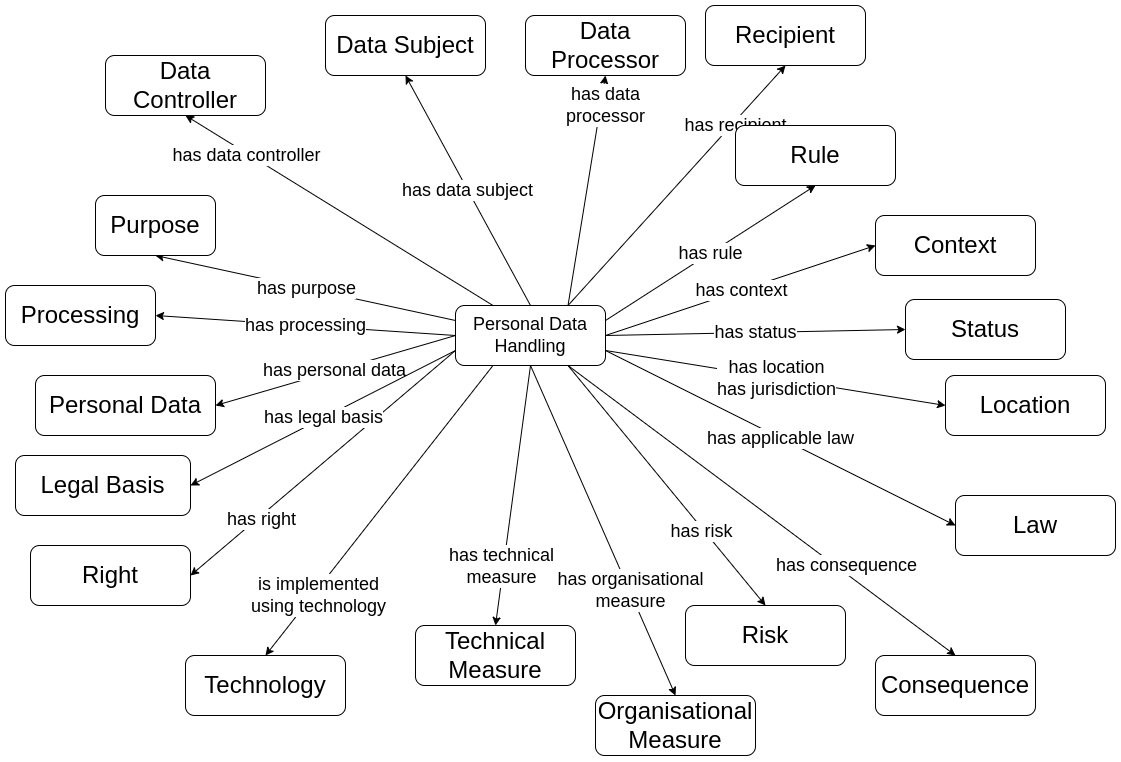
\includegraphics[width=0.8\textwidth]{figures/chapter-4/dpv-base.png}
\end{figure}

As indicated in the state of the art Chapter of this Thesis, DPV provides the most extensive list of data protection-related terms among the evaluated solutions.
Table \ref{tab:dpv_main_contributions} includes a list of the taxonomies defined in DPV's main specification, as well as the number of classes and properties defined in each taxonomy and, in the third column, the number of classes and properties which were contributed to the vocabulary in the course of the development of this Thesis. 

\begin{table}[htbp]
\centering
\caption[Taxonomies defined in DPV's main specification.]{Taxonomies defined in DPV's main specification, with the respective number of defined classes and properties, as well as the number of contributions of this Thesis to the vocabulary.}
\label{tab:dpv_main_contributions} 
\begin{tabular}{ c||c|c}
 Taxonomies & \#Classes (\#Properties)  & Contributions \\
 \hline\hline
 Entities & 4 (7) & 1 (4) \\
 \hline
 Legal Roles & 9 (9) & 0 (0) \\
 \hline
 Authorities & 5 (2) & 0 (0) \\
 \hline
 Organisations & 9 (0) & 0 (0) \\
 \hline
 Data Subjects & 26 (2) & 17 (0) \\
 \hline
 Purposes & 78 (2) & 20 (0) \\
 \hline
 Processing & 45 (1) & 0 (0) \\
 \hline
 Storage Conditions \& Automation & 29 (5) & 3 (0) \\
 \hline
 Scale of Processing & 27 (4) & 0 (0) \\
 \hline
 Data & 16 (2) & 0 (0) \\
 \hline
 TOMs & 139 (6) & 4 (0) \\
 \hline
 Legal Bases & 34 (5) & 0 (0) \\
 \hline
 Duration \& Frequency & 23 (11) & 7 (3) \\
 \hline
 Status & 39 (5) & 0 (0) \\
 \hline
 Location \& Jurisdiction & 25 (5) & 0 (0) \\
 \hline
 Risk \& Impacts & 16 (12) & 4 (3) \\
 \hline
 Rights & 9 (2) & 9 (0) \\
 \hline
 Rules & 4 (4) & 4 (4) \\
\end{tabular}
\end{table}

Moreover, the DPVCG also published a primer document \citep{pandit_primer_2022}, which provides a description of DPV and its concept modelling, examples which illustrate how the provided concepts should be used to represent metadata regarding personal data handling activities and guidelines towards the application of DPV in particular use cases, e.g., consent record keeping or rights exercising.
Additionally, as previously described in \ref{sec:dpv}, the DPVCG developed six extensions to the main specification, to model personal data categories, GDPR-specific concepts, technology and jurisdiction-relevant concepts, risk and EU rights concepts.
Table \ref{tab:dpv_extensions_contributions} includes a list of the DPV's extensions, as well as the number of classes and properties defined in each extension and, in the third column, the number of classes and properties which were contributed to the extensions in the course of the development of this Thesis.

\begin{table}[htbp]
\centering
\caption[DPV's extensions.]{DPV's extensions with the respective number of defined classes and properties, as well as the number of contributions of this Thesis to the extensions.}
\label{tab:dpv_extensions_contributions} 
\begin{tabular}{ c||c|c}
 Extensions & \#Classes (\#Properties)  & Contributions \\
 \hline\hline
 Personal data & 206 (0) & 3 (0) \\
 \hline
 GDPR & 92 (0) & 16 (0) \\
 \hline
 Technology & 60 (8) & 0 (0) \\
 \hline
 Jurisdiction & 452 (0) & 0 (0) \\
 \hline
 Risk & 376 (0) & 0 (0) \\
 \hline
 EU Rights & 62 (0) & 0 (0) \\
\end{tabular}
\end{table}

Additionally, existing work, using ODRL's profile mechanism, has been published to instantiate GDPR Articles as ODRL obligations~\citep{agarwal_legislative_2018} and as permissive, prohibitive or obligated policies with dispensations, which are translated into Answer Set Programming (ASP) rules for compliance checking~\citep{de_vos_odrl_2019}.
Other ODRL-based works have been published, related to (i) the representation of agreements to access data and execute algorithms in digital marketplaces~\citep{shakeri_modeling_2019}, (ii) the dynamic generation of privacy policies for IoT-generated data~\citep{canobenito_injecting_2023}, and (iii) the representation of privacy policies as ODRL requests, which use a small subset of DPV's taxonomies and do not follow the ODRL Information Model~\citep{krasnashchok_towards_2020}.
\section{ODRL profile for Access Control}
\label{sec:oac}

This Section describes the development of OAC, an ODRL profile for Access Control, to express access policies associated with data stored in decentralised datastores.

\subsection{Profile requirements specification}
\label{sec:oac_requirements}

This Section outlines the motivation and identified requirements for the development of the OAC profile.
As previously mentioned, personal datastores, such as Solid Pods, need to deal with GDPR's requirements, particularly the information requirements set out in Articles 13 and 14, such as the identity of the controller, the purpose for processing, the personal data categories being processed, or the legal basis being used, if they are to be adopted as a legally compatible solution for the sharing of personal data in Europe.
Taking Solid as a use case, this information can be given to Solid users by employing conventional methods, such as a notice provided through the data requester's website.
However, for individuals to control their data practices, the Solid Pod must also record this information so that the individual has the opportunity to:

\begin{enumerate}
    \item [(i)] inspect their personal data within an environment under their control;
    \item [(ii)] store it for accountability purposes;
    \item [(iii)] determine their data access preferences; and
    \item [(iv)] be assisted in enforcing said preferences.
\end{enumerate}

To achieve this, it is necessary to understand the provisions of the law regarding the information that needs to be provided, including the particular requirements of certain legal bases such as consent, and the forms of control that individuals want to have or the information they want to know in the context of the handling of their personal data.
Therefore, based on these considerations, the usage of ODRL and DPV is motivated by the following needs: 

\begin{itemize}
  \item[1.]Organisations need to:
    \begin{itemize}
      \item[a)]Specify machine-readable data handling policies, which should be accessible by users;
      \item[b)]Document provenance information related to their personal data processing activities, including notices and activity logs;
      \item[c)]Determine and fulfil applicable rights and obligations based on specific data protection laws or other contextual information, e.g., specific categories of personal data;
      \item[d)]Implement security measures by default and by design, specifically related to personal data access.
    \end{itemize}

    \item[2.]Users need to:
    \begin{itemize}
      \item[a)]Express human-centric data-sharing preferences, e.g., willingness to share a specific data type for non-profit research or to prohibit processing for profiling purposes;
      \item[b)]Specify broad permissions, e.g., allow data access for scientific research, or restrict third party data collection;
      \item[c)]Specify narrow permissions, e.g., allow access to phone contact details for a particular app, or deny access to a specific resource;
      \item[d)]Have a policy conflict strategy, e.g., generally deny access to location data, but include an exception for specific applications;
      \item[e)]Understand who is using which data categories, for what purposes, sharing it with whom, and under what legal basis.
    \end{itemize}
    
\end{itemize}

Moreover, taking into consideration the previously described motivation points, the following requirements can then be specified for the OAC profile:

\begin{itemize}
      \item[R1.]Support specifying user preferences as policies.
      \item[R2.]Incorporate vocabulary specifying or aligned to legal concepts.
      \item[R3.]Support specifying permissions and prohibitions at arbitrary granularity.
      \item[R4.]Support identifying and resolving conflicts based on scope.
      \item[R5.]Record policies used to authorise access to data.
      \item[R6.]Support querying policies and authorisations for introspection of data access.
\end{itemize}

As such, following the LOT methodology, these requirements are consolidated in the profile's ORSD available in Table \ref{tab:OAC_ORSD}.
As Solid's current access control mechanisms only partially implement R1, R3, and R5, OAC allows its users to declare not only granular permissive policies but also prohibitive policies, both aligned with legal requirements, which can be stored in their decentralised datastores for future inspection and can be used with additional constraints and contextual information.

\begin{table}[htbp]
\centering
\caption{Ontology Requirement Specification Document of the OAC profile.}
\label{tab:OAC_ORSD}
\scriptsize
\begin{tabular}{| l | l | l | l  | l | l | l |l| }
\hline
\multicolumn{8}{|c|}{\cellcolor[HTML]{A0A0A0}\textbf{ODRL Profile for Access Control}} \\ \hline
\multicolumn{8}{|c|}{\cellcolor[HTML]{EFEFEF}\textbf{1. Purpose}} \\ \hline
\multicolumn{8}{| p{12.0cm} |}{The purpose of this profile of ODRL is to support policies determining the access to personal data stored in decentralised storage environments, such as Solid Pods.} \\ \hline
\multicolumn{8}{|c|}{\cellcolor[HTML]{EFEFEF}\textbf{2. Scope}} \\ \hline
\multicolumn{8}{| p{12.0cm} |}{The scope of this profile is limited to the definition of an ODRL Profile for Access Control in decentralised settings. In particular, the introduced elements will serve one of these purposes: (i) define actions supporting the enforcement of current ACL verbs, (ii) define data protection-related actions and restrictions defined in GDPR, (iii) any vocabulary element to support policy patterns that can be anticipated to be common, and (iv) elements necessary to support the authorisation reasoning decision. } \\ \hline
\multicolumn{8}{|c|}{\cellcolor[HTML]{EFEFEF}\textbf{3. Implementation Language}} \\ \hline
\multicolumn{8}{| p{12.0cm} |}{RDF, RDFS} \\ \hline
\multicolumn{8}{|c|}{\cellcolor[HTML]{EFEFEF}\textbf{4. Intended End-Users}} \\ \hline
\multicolumn{8}{| p{12.0cm} |}{Developers of decentralised storage servers and applications, such as Solid servers and apps.} \\ \hline
\multicolumn{8}{|c|}{\cellcolor[HTML]{EFEFEF}\textbf{5. Intended Uses}} \\ \hline
\multicolumn{8}{| p{12.0cm} |}{
Use 1. Declaration of a policy by an individual storing personal data in a decentralised datastore, such as a Solid Pod. \newline 
Use 2. Request of data made by an entity, service or application to gain access to the data in different modalities. \newline
Use 3. Records of data access with transparent information related to the policy matching algorithm, including contextual information. 
 } \\ \hline
\multicolumn{8}{|c|}{\cellcolor[HTML]{EFEFEF}\textbf{6. Ontology Requirements}} \\ \hline
\multicolumn{8}{|c|}{\cellcolor[HTML]{EFEFEF}\textbf{a. Non-Functional Requirements}}    \\ \hline
\multicolumn{8}{| p{12.0cm} |}{
NFR 1. The profile is published online with HTML documentation, following W3C's specification format. } \\ \hline
\multicolumn{8}{|c|}{\cellcolor[HTML]{EFEFEF}\textbf{b. Functional  Requirements: Groups of Competency Questions}}  \\ \hline
\multicolumn{5}{|c|}{\cellcolor[HTML]{EFEFEF}CQG1. Related to access} & \multicolumn{3}{|c|}{\cellcolor[HTML]{EFEFEF}CQG2. Related to GDPR} \\ \hline %\multicolumn{4}{c|}{\cellcolor[HTML]{EFEFEF}}    \\ \hline
\multicolumn{5}{ | m{7cm} |}{
CQ1. Which policy type is being defined? \newline
CQ2. Which actions are defined in the policy? \newline
CQ3. Which data types are mentioned in the policy? \newline 
CQ4. Which policy constraints need to be fulfilled? \newline 
CQ5. Who are the parties intervening in the policy? \newline 
CQ6. Which is the conflict strategy of a policy? \newline 
CQ7. What are the contextual elements that need to be considered in the policy matching algorithm? } & 
\multicolumn{3}{ m{5cm} |}{
CQ8. Which information about personal data and its processing is necessary to have legally aligned policies? \newline 
CQ9. What identification information needs to be provided by the policy parties? \newline 
}\\ \hline
\end{tabular}
\vspace{-0.1in}
\end{table}

%For continued interoperability and adherence to the specification, the proposed extension to Solid’s ACL must ideally continue to implement existing functionality while incorporating the legal and user-centric requirements.

Lastly, it should be clear that OAC is \textbf{not dependent on Solid}, as it is not based on any Solid-specific vocabularies, and can be used in other decentralised data environments.
Nevertheless, throughout this Thesis, the use of OAC is demonstrated through the Solid ecosystem as it is an example of the implementation of a decentralised environment for the sharing of (personal) data that is based on the Semantic Web stack of technologies.

\subsection{Profile implementation}
\label{sec:oac_implementation}

This ODRL profile relies on DPV, for the invocation of legal concepts related to data protection and privacy, and ACL, for the expression of access mode operations, to specify complex permissions, prohibitions or duties over the access to personal data resources.

Moreover, OAC policies can be used to add a new layer to decentralised data systems -- a layer that is currently missing from the Solid ecosystem for instance -- that will come between the data and the access authorisation, e.g., ACL or ACP authorisations, layers in order to provide a richer access control mechanism to such systems.
As an access control mechanism's main goal is to determine access by users or software agents to digital resources, the entities generating and/or providing the data must able to express policies that satisfy their preferences, while users or software agents who wish to access said data must be able to define policies that describe their data handling activities. 
By using these policies in an algorithm to match incoming access requests for data, an agreement over the access to a certain resource or type of data can be defined and the decentralised data system can provide a fine-grained access control mechanism to its users.
As such, OAC reuses ODRL's \texttt{Offer} policies to express the conditions for access to personal data stored in decentralised data systems, e.g. Solid Pods, \texttt{Request} policies to express users or software agents' access requests and \texttt{Agreement} policies to describe the agreed conditions for access to the data. 
The three types of policies are defined below, according to their definition provided in the ODRL Vocabulary \& Expression 2.2 Recommendation specification \citep{iannella_odrl_vocab_2018}:

\begin{itemize}
    \item \textbf{Offer} -- Policy that proposes the assigner's rules over an asset and does not grant any privileges to assignees.
    \item \textbf{Request} -- Policy that proposes the assignee's rules over an asset and does not grant any privileges to any parties.
    \item \textbf{Agreement} -- Policy issued by an assigned that grants privileges to the assignee over an asset.
\end{itemize}

OAC's core concepts are illustrated in Figure~\ref{fig:oac_diagram} and Tables \ref{tab:profile_classes} and \ref{tab:profile_properties} specify the alignment between the ODRL, DPV, and ACL terms to ensure that their semantics are correctly interpreted by OAC implementers.

%Its core concepts are the Preference and Requirement policies, a new set of operators to constraint the defined Purposes, Recipients, Legal Basis, Technical and Organisational Measures, Technology and Identity Provider constraints (which will require the usage of DPV's taxonomies), new properties to specify policies for applications and services, Processing and Access actions, as well as Personal Data Categories, and Legal Entities.

\begin{figure}[htbp]
    \centering
    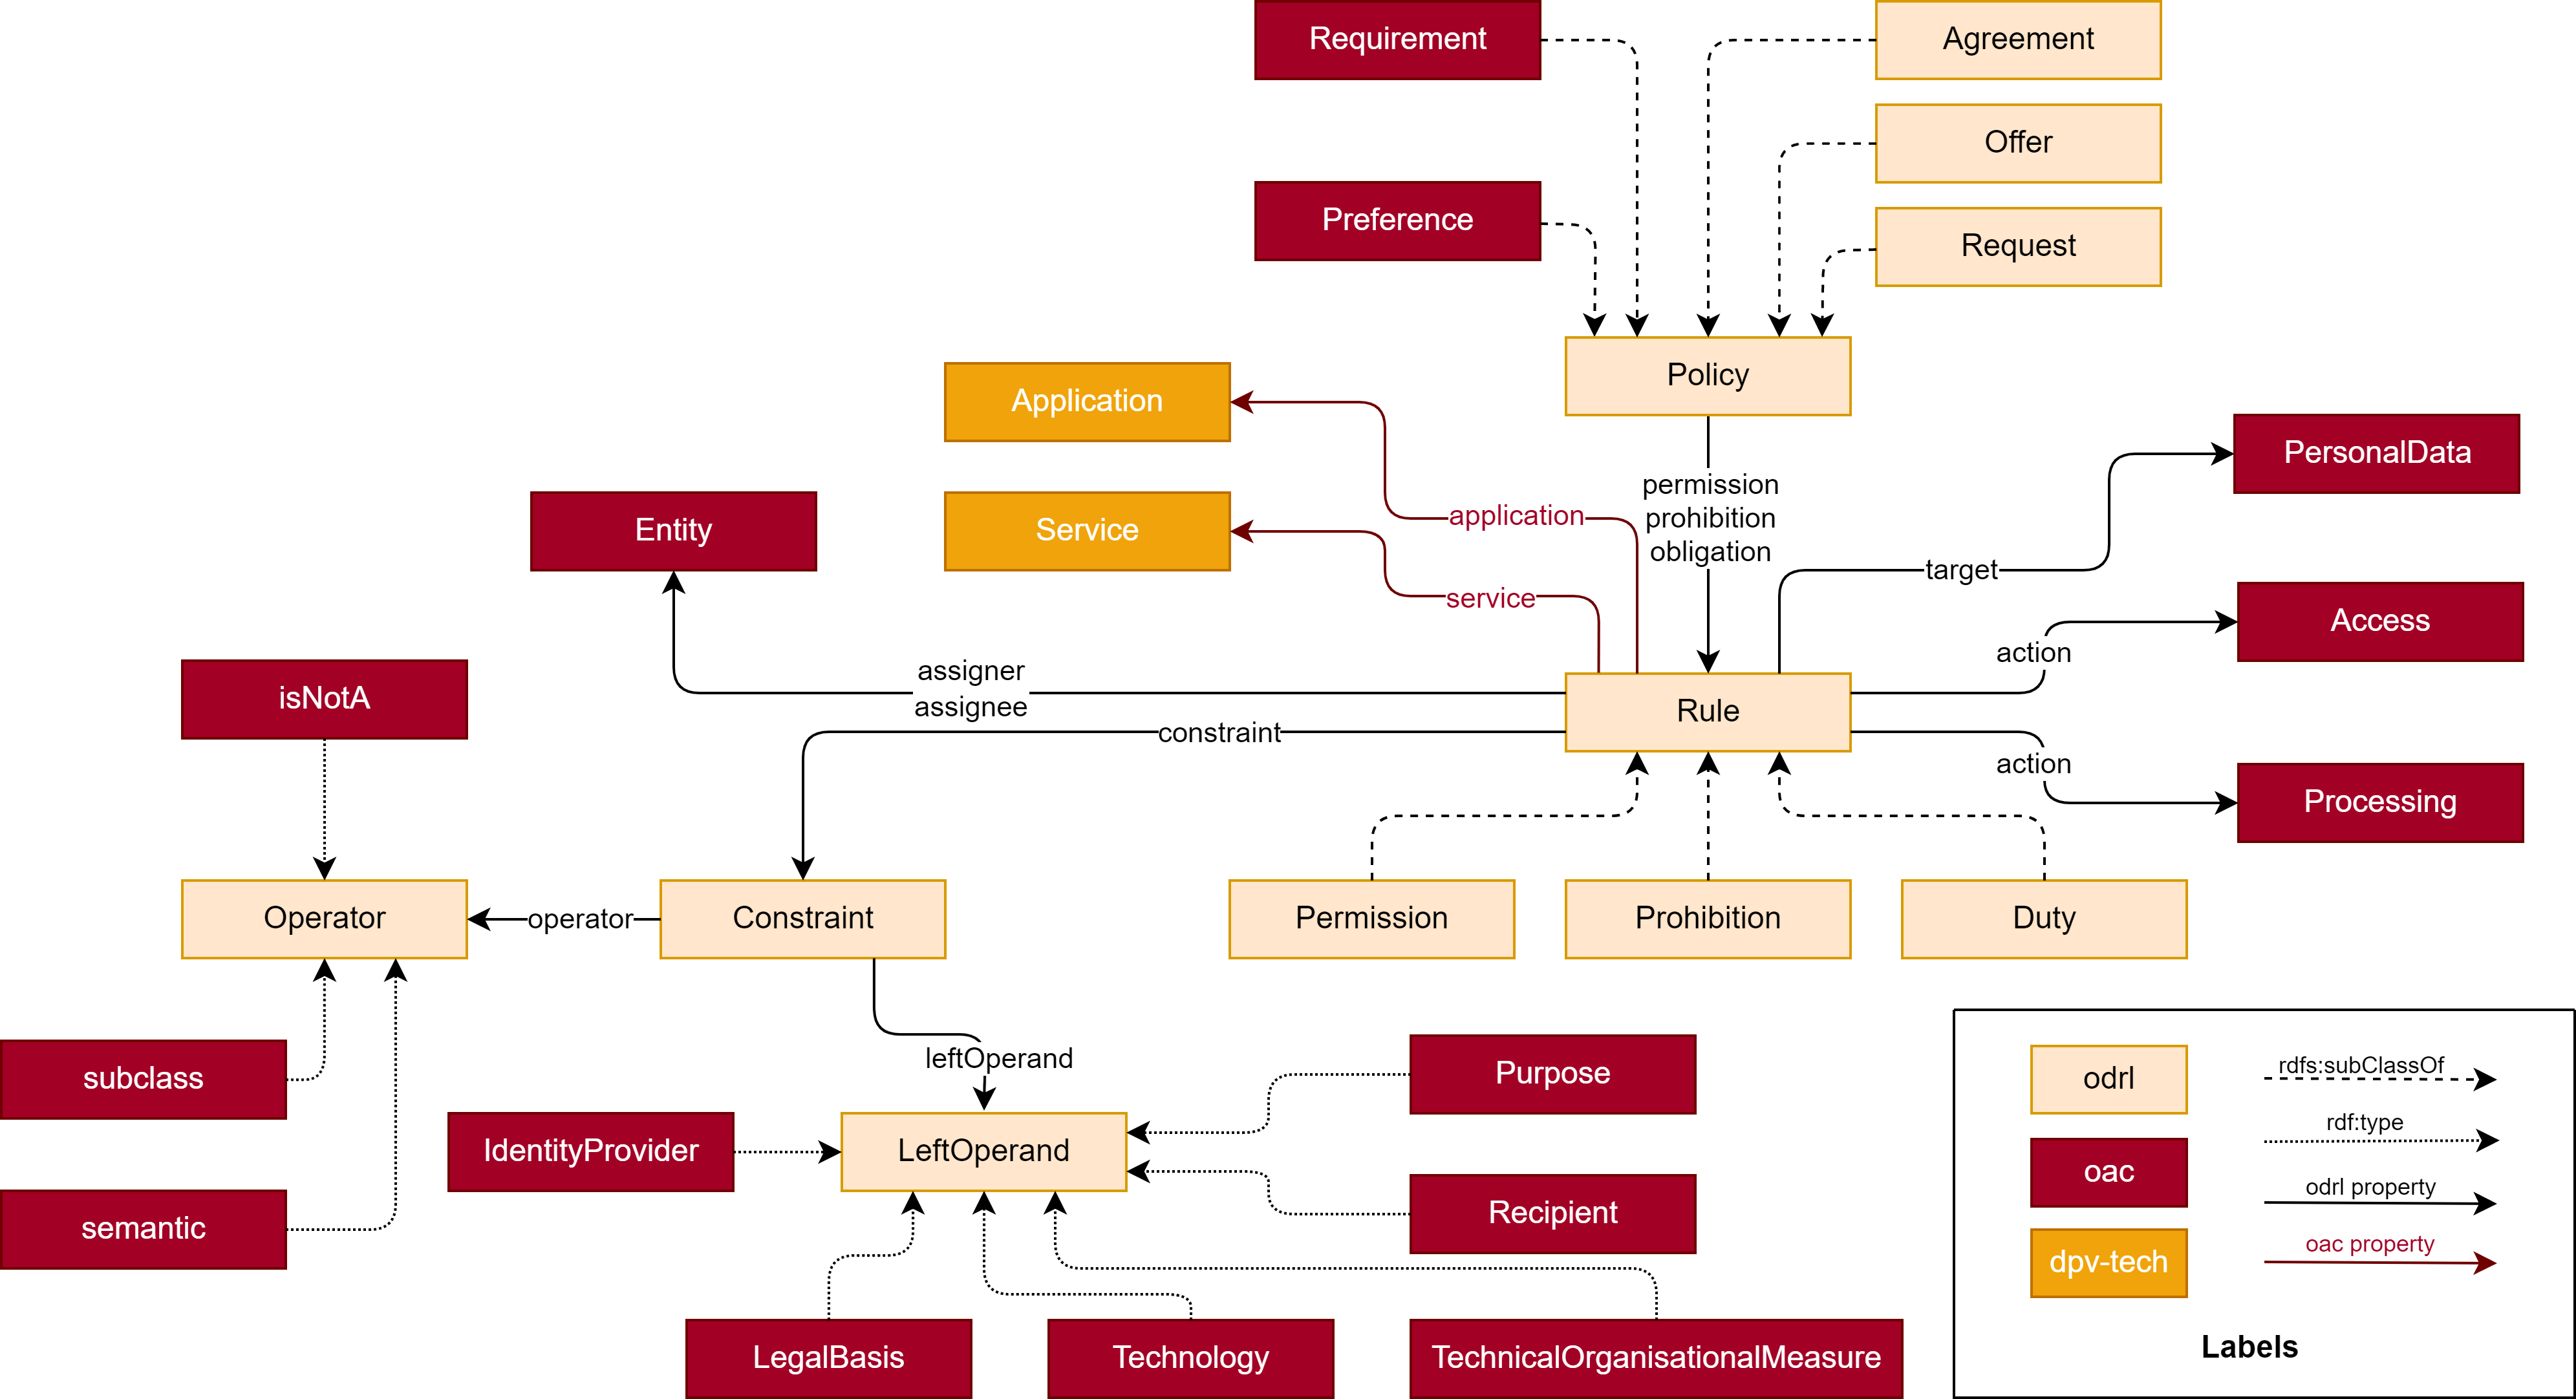
\includegraphics[width=\linewidth]{figures/chapter-4/oac_diagram.png}
    \caption{Diagrams of the concepts specified by the OAC profile.}
    \label{fig:oac_diagram}
\end{figure}

Two new types of policies, which can be combined in ODRL offers, are specified to deal with the preferences and requirements of users who wish to define rules for the processing of their personal data:

\begin{itemize}
    \item \textbf{Preference} -- Soft policy that expresses the assigner's preferences over a personal data asset which may not be satisfied and must not grant any privileges to assignees. If a preference policy set by party A does not match a request policy from party B, the request can still be accepted if party A accepts party B's request conditions.
    \item \textbf{Requirement} -- Hard policy that expresses the assigner's preferences over a personal data asset which must be satisfied and must not grant any privileges to assignees. If a requirement policy set by party A does not match a request policy from party B, the request must be denied even if party A accepts party B's request conditions.
\end{itemize}

\begin{table}[htbp]
\centering
\caption{Classes and named individuals specified in the OAC profile.}
\label{tab:profile_classes}
\resizebox{\textwidth}{!}{
\begin{tabular}{c||c|c}
Profile term & Instance of & Subclass of \\
\hline\hline
\texttt{oac:Preference} & & \texttt{odrl:Policy} \\
\hline
\texttt{oac:Requirement} & & \texttt{odrl:Policy} \\
\hline
\texttt{oac:isNotA} & \texttt{odrl:Operator} & \\
\hline
\texttt{oac:subclass} & \texttt{odrl:Operator} & \\
\hline
\texttt{oac:semantic} & \texttt{odrl:Operator} & \\
\hline
\texttt{oac:PersonalData} & \texttt{odrl:Asset} & \texttt{dpv:PersonalData} \\
\hline
\texttt{oac:Access} & \texttt{odrl:Action} & \texttt{acl:Access} \\
\hline
\texttt{oac:Processing} & \texttt{odrl:Action} & \texttt{dpv:Processing} \\
\hline
\texttt{oac:Entity} & \texttt{odrl:Party} & \texttt{dpv:Entity} \\
\hline
\texttt{oac:Purpose} & \texttt{odrl:LeftOperand} & \texttt{dpv:Purpose} \\
\hline
\texttt{oac:Recipient} & \texttt{odrl:LeftOperand} & \texttt{dpv:Recipient} \\
\hline
\texttt{oac:LegalBasis} & \texttt{odrl:LeftOperand} & \texttt{dpv:LegalBasis} \\
\hline
\texttt{oac:TechnicalOrganisationalMeasure} & \texttt{odrl:LeftOperand} & \texttt{dpv:TechnicalOrganisationalMeasure} \\
\hline
\texttt{oac:Technology} & \texttt{odrl:LeftOperand} & \texttt{dpv:Technology} \\
\hline
\texttt{oac:IdentityProvider} & \texttt{odrl:LeftOperand} & \\
\end{tabular}}
\end{table}

\begin{table}[htbp]
\centering
\caption{Properties specified in the OAC profile.}
\label{tab:profile_properties}
\begin{tabular}{c||c|c}
Profile property & Domain & Range \\
\hline\hline
\texttt{oac:service} & \texttt{odrl:Rule}, \texttt{odrl:Policy} & \texttt{dpv-tech:Service} \\
\hline
\texttt{oac:application} & \texttt{odrl:Rule}, \texttt{odrl:Policy} & \texttt{dpv-tech:Application} \\
\end{tabular}
\end{table}

Listing~\ref{list:oac_req_pref} presents an example of an OAC requirement and an OAC preference policies and Listing~\ref{list:oac_offer} an ODRL offer, based on the previously listed requirement and preference policies, as is indicated by the \texttt{dcterms:source} property.
The permission associated with the requirement policy contains the property \texttt{dpv:hasContext} associated with the term \texttt{dpv:Required} to indicate that said permission is a requirement, while the term \texttt{dpv:Optional} is used to identify the rules related with a preference policy.

\begin{listing}[htp]
\caption{OAC requirement and preference policies issued by \url{https://solidweb.me/besteves4/profile/card\#me}.}
\label{list:oac_req_pref}
\begin{minted}{turtle}
<https://solidweb.me/besteves4/policies/requirement1> a oac:Requirement ;
    odrl:uid <https://solidweb.me/besteves4/policies/requirement1> ;
    odrl:profile oac: ;
    dcterms:description "Requirement to read identifier data for identity verification purposes." ;
    dcterms:creator <https://solidweb.me/besteves4/profile/card#me> ;
    dcterms:issued "2023-10-20T18:22:15"^^xsd:dateTime ;
    odrl:permission [
        odrl:assigner <https://solidweb.me/besteves4/profile/card#me> ;
        odrl:target oac:Identifier ;
        odrl:action oac:Read ;
        odrl:constraint <#Constraint_Purpose_IdentityVerification> .

<#Constraint_Purpose_IdentityVerification> a odrl:Constraint ;
    dcterms:title "Purpose for access is to verify the identity of the assigner." ;
    odrl:leftOperand oac:Purpose ;
    odrl:operator odrl:isA ;
    odrl:rightOperand dpv:IdentityVerification .

<https://solidweb.me/besteves4/policies/preference1> a oac:Preference ;
    odrl:uid <https://solidweb.me/besteves4/policies/preference1> ;
    odrl:profile oac: ;
    dcterms:description "Preference to read age data if purpose is not commercial research." ;
    dcterms:creator <https://solidweb.me/besteves4/profile/card#me> ;
    dcterms:issued "2023-10-20T18:26:09"^^xsd:dateTime ;
    odrl:permission [
        odrl:assigner <https://solidweb.me/besteves4/profile/card#me> ;
        odrl:target oac:Age ;
        odrl:action oac:Read ;
        odrl:constraint <#Constraint_Purpose_not_CommercialResearch> .

<#Constraint_Purpose_not_CommercialResearch> a odrl:Constraint ;
    dcterms:title "Purpose for access is not commercial research." ;
    odrl:leftOperand oac:Purpose ;
    odrl:operator oac:isNotA ;
    odrl:rightOperand dpv:CommercialResearch .
\end{minted}
\end{listing}

\begin{listing}[htp]
\caption{ODRL offer issued by \url{https://solidweb.me/besteves4/profile/card\#me}.}
\label{list:oac_offer}
\begin{minted}{turtle}
<https://solidweb.me/besteves4/policies/offer1> a odrl:Offer ;
    odrl:uid <https://solidweb.me/besteves4/policies/offer1> ;
    odrl:profile oac: ;
    dcterms:description "Offer to read identifier data for identity verification and age data if purpose is not commercial research." ;
    dcterms:creator <https://solidweb.me/besteves4/profile/card#me> ;
    dcterms:source <https://solidweb.me/besteves4/policies/requirement1>, <https://solidweb.me/besteves4/policies/preference1> ;
    dcterms:issued "2023-10-20T22:15:34"^^xsd:dateTime ;
    odrl:permission [
        dpv:hasContext dpv:Required ;
        odrl:assigner <https://solidweb.me/besteves4/profile/card#me> ;
        odrl:action oac:Read ;
        odrl:target oac:Identifier ;
        odrl:constraint <#Constraint_Purpose_IdentityVerification>
    ] ;
    odrl:permission [
        dpv:hasContext dpv:Optional ;
        odrl:assigner <https://solidweb.me/besteves4/profile/card#me> ;
        odrl:action oac:Read ;
        odrl:target oac:Age ;
        odrl:constraint <#Constraint_Purpose_not_CommercialResearch>
    ] .

<#Constraint_Purpose_IdentityVerification> a odrl:Constraint ;
    dcterms:title "Purpose for access is to verify the identity of the assigner." ;
    odrl:leftOperand oac:Purpose ;
    odrl:operator odrl:isA ;
    odrl:rightOperand dpv:IdentityVerification .

<#Constraint_Purpose_not_CommercialResearch> a odrl:Constraint ;
    dcterms:title "Purpose for access is not commercial research." ;
    odrl:leftOperand oac:Purpose ;
    odrl:operator oac:isNotA ;
    odrl:rightOperand dpv:CommercialResearch .
\end{minted}
\end{listing}

Additionally, a set of three new ODRL operators, which are currently missing from the ODRL Core vocabulary Recommendation, and two new properties to specify policies applicable to certain services or applications, \texttt{oac:service} and \texttt{oac:application}, which are important stakeholders in decentralised data systems, are specified in OAC.
The newly introduced \texttt{oac:isNotA} operator is used in the \texttt{<\#Constraint\_Purpose\_not\_CommercialResearch>} constraint, in Listing~\ref{list:oac_req_pref}, to indicate that the purpose for access can not be an instance of the right operand of the constraint, e.g., \texttt{dpv:CommercialResearch}.
The \texttt{oac:subclass} operator can be used to indicate that a given left operand is a subclass of the right operand of the constraint, e.g., the purpose constraint of a rule can be a subclass of DPV's research and development purpose such as academic research, non-commercial research or commercial research, and the \texttt{oac:semantic} operator to express that a given left operand is equal to, an instance or a subclass of the right operand of the constraint, e.g., the purpose constraint of a rule can be research and development, an instance of research and development or one of its subclasses such as academic research, non-commercial research or commercial research.

Personal data is defined as an ODRL asset to define personal data-specific access policies, access modes and processing operations are defined as ODRL actions to define policies for specific access modes and/or processing operations which are not covered by ACL's access modes, e.g., \texttt{dpv:Transfer} or \texttt{dpv:Copy}, and DPV's \texttt{Entity} concept is defined as an ODRL party to define entity-specific access policies.
Additionally, when defining ODRL requests, the data requesters might use processing concepts, \texttt{dpv:Use, dpv:Collect, dpv:Share}, as the permitted/prohibited action of the rule that differ from the existing ACL's access modes, \texttt{acl:Read, acl:Write, acl:Append}.
As such, a mapping of ACL verbs to DPV processing operations is provided in OAC for such cases where offers and requests need to be matched and include both ACL access modes and DPV processing operations.
In this mapping, the \texttt{acl:Read} access mode corresponds to \texttt{dpv:Use, dpv:Collect} processing operations, and \texttt{acl:Write} resembles \texttt{dpv:Store, dpv:MakeAvailable}.
Furthermore, as previously mentioned, there are operations such as \texttt{dpv:Share} or \texttt{dpv:Transfer} that do not have a specific corresponding concept in WAC's ACL vocabulary, which require a greater introspection in the integration of legal processing concepts with access control operations.
Moreover, purposes, recipients, legal bases, technical and organisational measures, technologies and identity providers are defined as ODRL constraints to define constraint-restricted access policies.

Listing~\ref{list:oac_request} presents an example of an ODRL request that uses OAC terms and Listing~\ref{list:oac_agreement} an ODRL agreement which is the result of the matching between the offer defined in Listing~\ref{list:oac_offer} and the previously mentioned request.
In this example, Beatriz, identified by \url{https://solidweb.me/besteves4/profile/card#me}, and Arya, identified by \url{https://solidweb.me/arya/profile/card#me}, reach an agreement to allow read access operations over Beatriz's age data for the purpose of academic research in project X.
This \texttt{odrl:Agreement} is the result of the matching of \url{https://solidweb.me/besteves4/policies/offer1} and \url{https://solidweb.me/arya/requests/age_academicResearch}, as indicated by the \texttt{dcterms:references} property.
The legal basis of the agreement is consent, as is specified in the policy with the \texttt{dpv:hasLegalBasis dpv:Consent} terms, and Beatriz and Arya are registered as the data subject and data controller in question, respectively, using the \texttt{dpv:hasDataSubject} and \texttt{dpv:hasDataController} terms.
\beatriz{Policy matching and agreement generation is discussed in Chapter XX.}

\begin{listing}[ht]
\caption{ODRL request issued by \url{https://solidweb.me/arya/profile/card\#me}.}
\label{list:oac_request}
\begin{minted}{turtle}
<https://solidweb.me/arya/requests/age_academicResearch> a odrl:Request ;
    odrl:uid <https://solidweb.me/arya/requests/age_academicResearch> ;
    odrl:profile oac: ;
    dcterms:description "Request to read age data for academic research." ;
    dcterms:creator <https://solidweb.me/arya/profile/card#me> ;
    dcterms:issued "2023-10-21T13:47:56"^^xsd:dateTime ;
    odrl:permission [
        odrl:assignee <https://solidweb.me/arya/profile/card#me> ;
        odrl:action oac:Use ;
        odrl:target oac:Age ;
        odrl:constraint <#Constraint_Purpose_AcademicResearch>
    ] .

<#Constraint_Purpose_AcademicResearch> a odrl:Constraint ;
    dcterms:title "Purpose for access is to conduct academic research in project X." ;
    odrl:leftOperand oac:Purpose ;
    odrl:operator odrl:eq ;
    odrl:rightOperand ex:AcademicResearchProjectX .

ex:AcademicResearchProjectX a dpv:Purpose ;
    rdfs:subClassOf dpv:AcademicResearch ;
    rdfs:label "Conduct research in the academic project X." .
\end{minted}
\end{listing}

\begin{listing}[ht]
\caption{ODRL agreement to read age data for academic research based on consent.}
\label{list:oac_agreement}
\begin{minted}{turtle}
<https://solidweb.me/besteves4/policies/agreement1> a odrl:Agreement ;
    odrl:uid <https://solidweb.me/besteves4/policies/agreement1> ;
    odrl:profile oac: ;
    dcterms:description "Agreement to read age data for academic research based on consent." ;
    dcterms:creator <https://solidweb.me/besteves4/profile/card#me> ;
    dcterms:issued "2023-10-21T13:58:37"^^xsd:dateTime ;
    dcterms:references <https://solidweb.me/besteves4/policies/offer1>, <https://solidweb.me/arya/requests/age_academicResearch> ;
    dpv:hasDataSubject <https://solidweb.me/besteves4/profile/card#me> ;
    dpv:hasDataController <https://solidweb.me/arya/profile/card#me> ;
    dpv:hasLegalBasis dpv:Consent ;
    odrl:permission [
        odrl:assigner <https://solidweb.me/besteves4/profile/card#me> ;
        odrl:assignee <https://solidweb.me/arya/profile/card#me> ;
        odrl:action oac:Read ;
        odrl:target oac:Age ;
        odrl:constraint <#Constraint_Purpose_AcademicResearch>
    ] .
\end{minted}
\end{listing}

This Thesis focuses on \textit{Purpose, Personal Data, Processing, Recipients, Legal Bases, Technical and Organisational Measures} and \textit{Technologies} as the minimum `core concepts' for the OAC profile, and leaves out other DPV concepts such as rights or risks, which can be added at a later stage if needed.
Furthermore, similarly to WAC and ACP, OAC policies can also be defined for particular resources identified by URIs -- in such cases when an access request for a particular data type comes in, the authorisation mechanism must have information about what type of data those particular resources contain or else they will not be returned if they match the data type of the request.
Such information can be stored in a data registry, stored in a e.g. Solid Pod, where resources can be associated with the type of data they contain by using DPV's \texttt{hasPersonalData} property and DPV-PD's taxonomy of personal data categories, e.g., \texttt{<https://solidweb.me/besteves4/private/health/file1> dpv:hasPersonalData dpv-pd:HealthHistory .}

Ultimately, since these policies are stored in the personal datastore for purposes of accountability and transparency, apps and services, based on the stored preferences, requests, and agreements, can be built, e.g., using SPARQL queries, to inquire who is using what data and for what purposes.
Listing~\ref{list:sparql_agreement} presents a SPARQL query to retrieve permitted data accesses by user, data, and purpose from ODRL agreements stored in a decentralised datastore.

\begin{listing}[ht]
\caption{SPARQL query to retrieve authorised data accesses by user, data, and purpose.}
\label{list:sparql_agreement}
\begin{minted}{sparql}
SELECT DISTINCT ?User ?Data ?Purpose WHERE {
    ?a a odrl:Agreement .
    ?a odrl:permission ?perm .
    ?perm odrl:assignee ?User .
    ?perm odrl:target ?Data .
    ?perm odrl:constraint ?c .
    ?c odrl:leftOperand oac:Purpose .
    ?c odrl:operator odrl:eq .
    ?c odrl:rightOperand ?Purpose .
}
\end{minted}
\end{listing}

\subsection{Profile publication and maintenance}
\label{sec:oac_publication}

The ontology human-readable documentation and machine-readable file are available at \url{https://w3id.org/oac} using content negotiation.
The HTML documentation includes a description of the classes and properties of the ontology, that was done in collaboration with domain experts, a diagram with the graphical representation of the ontology, examples of policies defined with the OAC profile, and information related to the policy matching algorithm.
The ontology documentation also includes metadata, such as the identity of the creators and publishers of the ontology, the dates of creation and last modification, or the version number.

The source code is hosted at \url{https://w3id.org/oac/repo}, under the CC-BY-4.0 license.
The repository can also be used by OAC users to suggest new inclusions to the ontology and to report bugs through GitHub Issues.
In addition, the repository at \url{https://w3id.org/oac/policies} contains a growing collection of OAC policies that can be reused by OAC users.
\section{Metadata language for Solid}
\label{sec:plasma}

This Section describes the development of PLASMA, a metadata language for policy-based access control in Solid, to express metadata related to the entities, registries, logs, policies and infrastructure necessary to provide transparency to Solid's data handling practices.

\subsection{PLASMA requirements specification}
\label{sec:plasma_requirements}

This Section outlines the motivation and identified requirements for the development of PLASMA, a Policy LAnguage for Solid’s Metadata-based Access control.
As previously mentioned, Solid builds upon Web's ethical principles\footnote{\url{https://www.w3.org/TR/ethical-web-principles/} (accessed on 22 October 2023)} and standards such as LDP or RDF and, in accordance with its Protocol, relies on said standards to \textit{``realise a space where individuals can maintain their autonomy, control their data and privacy, and choose applications and services to fulfil their needs''} \citep{capadisli_solid_2022}.

Although it was designed with these goals in mind, Solid currently lacks compatibility with data protection regulatory efforts \citep{pandit_making_2023}, such as the GDPR.
In particular, Solid lacks a practical mechanism to enforce GDPR's principles of transparency and accountability as there are no tools for users, applications or services to model or document information related to privacy notices, agreements, consent and rights exercising.
Furthermore, Solid is based on a ground-up redesign where machine-readable information is encouraged to be provided and reused towards improving the value of data and quality of life for users.
However, Solid's access control specifications do not contain any mechanism by which apps can provide or users can understand or express information regarding who/why/how data will be used, and to utilise these in making the process of granting and controlling access to data easier and legally compatible.
This lack of `actionable records' also strengthens the propagation of existing problems of the Web such as the use of dark patterns or manipulations to gain access to personal data of Web users.

Given that users are well versed in the usage of apps, e.g. on their smartphones, there is an expectation that Solid should also adopt an environment of trust and accountability that reduces the cognitive overload on users to understand complex information and make informed decisions, and where the environment guides responsible and accountable development.
Examples of such measures include the usage of app stores and curated or approved application verification processes.
Without these, Solid users currently have no means to identify who are the actors behind the app and authorities cannot know whom to approach when opening an investigation on faulty data practices.

Therefore, based on these considerations, the following requirements were drafted for the development of PLASMA:

\begin{enumerate}
    \item [R1.] Support specifying information about Solid infrastructure.
    \item [R2.] Record information about Pod, apps, services and data providers/developers.
    \item [R3.] Support specifying of different agreements and notices.
    \item [R4.] Record provenance information for future introspection and convenient access to data.
    \item [R5.] Provide conformance conditions to assist with legal compliance.
\end{enumerate}

As such, following the LOT methodology, these requirements are consolidated in the ORSD available in Table~\ref{tab:plasma_orsd}.
By incorporating the usage of PLASMA, Solid actors can describe their data practices in a responsible and accountable manner in a way that addresses the above-mentioned requirements.
In addition to providing the vocabulary, PLASMA also demonstrates how a \textit{decentralised ecosystem} can be developed that takes advantage of the machine-readable nature of RDF information, such as to guarantee that apps declare a set of metadata before being allowed access to data, and ensures that apps, services, agents, Pods and users act in conformance and provide an environment of trust and accountability.

\begin{table}[htbp]
\centering
\caption{Ontology Requirement Specification Document of PLASMA.}
\label{tab:plasma_orsd}
\scriptsize
\begin{tabular}{| l | l | l | l  | l | l | l |l| }
\hline
\multicolumn{8}{|c|}{\cellcolor[HTML]{A0A0A0}\textbf{Policy LAnguage for Solid’s Metadata-based Access control}} \\ \hline
\multicolumn{8}{|c|}{\cellcolor[HTML]{EFEFEF}\textbf{1. Purpose}} \\ \hline
\multicolumn{8}{| p{12.0cm} |}{The purpose of PLASMA is to provide consistent taxonomies to describe the entities, infrastructure, policies, notices, registries and logs necessary to understand and establish responsibilities and accountability within the Solid ecosystem.} \\ \hline
\multicolumn{8}{|c|}{\cellcolor[HTML]{EFEFEF}\textbf{2. Scope}} \\ \hline
\multicolumn{8}{| p{12.0cm} |}{The scope of this ontology is limited to the definition of a metadata language to provide transparency Solid's data handling practices. PLASMA promotes the usage of OAC to determine access control to Solid Pod's resources, provides conformance conditions and workflow scenarios where PLASMA terms should be used.} \\ \hline
\multicolumn{8}{|c|}{\cellcolor[HTML]{EFEFEF}\textbf{3. Implementation Language}} \\ \hline
\multicolumn{8}{| p{12.0cm} |}{RDF, RDFS} \\ \hline
\multicolumn{8}{|c|}{\cellcolor[HTML]{EFEFEF}\textbf{4. Intended End-Users}} \\ \hline
\multicolumn{8}{| p{12.0cm} |}{Developers of Solid servers, applications, services or agents.} \\ \hline
\multicolumn{8}{|c|}{\cellcolor[HTML]{EFEFEF}\textbf{5. Intended Uses}} \\ \hline
\multicolumn{8}{| p{12.0cm} |}{
Use 1. Describing entities, infrastructure and processes involved in the Solid ecosystem. \newline 
Use 2. Expressing information regarding legal roles and other compliance requirements in a jurisdiction-agnostic manner (while satisfying requirements from GDPR). \newline
Use 3. Defining patterns for the expression of users and apps policies, data use logs, and registries to provide easy access to data in Pods. 
 } \\ \hline
\multicolumn{8}{|c|}{\cellcolor[HTML]{EFEFEF}\textbf{6. Ontology Requirements}} \\ \hline
\multicolumn{8}{|c|}{\cellcolor[HTML]{EFEFEF}\textbf{a. Non-Functional Requirements}}    \\ \hline
\multicolumn{8}{| p{12.0cm} |}{
NFR 1. The ontology is published online with HTML documentation, following W3C's specification format. } \\ \hline
\multicolumn{8}{|c|}{\cellcolor[HTML]{EFEFEF}\textbf{b. Functional  Requirements: Groups of Competency Questions}}  \\ \hline
\multicolumn{8}{|p{12.0cm}|}{
CQ1. Which Pod management data is stored in the Pod? \newline
CQ2. Which metadata should be recorded when data is added/updated/removed to/from the Pod? \newline
CQ3. What data, including policies, are available in the Pod? \newline 
CQ4. What policy describes the data access requirements of a certain app or service? \newline 
CQ5. Who are the parties providing Pod infrastructure? \newline 
CQ6. How and where is the data being physically stored? \newline 
CQ7. What registries are available in the Pod for convenient access to data? \newline
CQ8. What identification information needs to be provided by Solid-involved parties? \newline 
CQ9. Which information about personal data processing is necessary to have legally aligned decentralised datastores?
}\\ \hline
\end{tabular}
\vspace{-0.1in}
\end{table}

\subsection{PLASMA taxonomies}
\label{sec:plasma_taxonomies}

PLASMA relies on OAC for the expression of policies related to access to personal data stored in Solid Pods, on the W3C Recommendation DCAT (Data CATalog vocabulary) \citep{albertoni_data_2020} for the expression of data registries and related data sets, on DCMI Metadata Terms \citep{dcmi_usage_board_dcmi_2020} for the specification of authorship, temporal and other types of provenance metadata, and on the W3C Recommendation Activity Streams 2.0 \citep{snell_activity_2017} for logging relevant events associated with Solid processes.
These design choices are aligned with the best practices described in the Data on the Web Best Practices document \citep{loscio_data_2017}.
Moreover, while there are legal vocabularies focusing on personal data protection, such as DPV and DPV-GDPR \citep{panetto_creating_2019}, these are not directly applicable to the Solid ecosystem as the terminology used is not the same, e.g., in Solid, the entity the data belongs/refers to is called \textit{`owner'}, whereas the equivalent term under the GDPR is \textit{`data subject'}.
As such, PLASMA provides additional taxonomies to describe the actors, artifacts, and processes involved in the usage of Solid Pods, apps and services, which are not modelled in the previously mentioned vocabularies.
Later on, these can be used to align with their equivalent legal terms (from the GDPR).

Thus, PLASMA supports the implementation of a new \textit{`policy layer'} which aids users, apps and Pod infrastructure providers to express relevant information about their activities in the form of machine-readable policies, logs and registers of data.
Such sources of information can then be used to enable the development of dashboards for user policy management, machine-readable notifications regarding changes in policies or data, usage of agents to automate tasks or other interfaces to understand what is being done with the Pod's data.

Figure~\ref{fig:solid_plasma} illustrates the core entities and infrastructure of the Solid ecosystem as specified in PLASMA.
Thus, the base PLASMA concepts are defined below as:

\begin{itemize}
    \item \textbf{App} -- An application that stores, collects, uses, shares, erases, or performs other actions on Data with the aim of providing specific purposes, services, or functionalities. An application can use several Services and requires human intervention.
    \item \textbf{Service} -- A functionality that may or may not utilise or interact with Data within a Pod. Services represent an abstraction of functionality that does not necessarily have to be packaged as an App.
\end{itemize}

\begin{landscape}
\begin{figure}[htbp]
    \centering
    \includegraphics[width=\linewidth]{figures/chapter-4/solid-infrastructure-actors.png}
    \caption{Core entities and infrastructure of the Solid ecosystem specified in PLASMA.}
    \label{fig:solid_plasma}
\end{figure}
\end{landscape}

\begin{itemize}
    \item \textbf{Pod} -- A Personal Data Store that conforms to the Solid Specification.
    \item \textbf{Agent} -- A virtual entity associated with carrying out actions within or related to a Pod or its Data.
    \item \textbf{Policy} -- A set of guidelines or decisions or recommendations governing the use of Pod or its Data.
    \item \textbf{Data} -- Data stored on a Pod or associated with a User, App, Service, or Data Subject of a Pod.
    \item \textbf{Entity} -- A legally recognised entity. Legally recognised means the entity has some recognition as being able to enter into agreements, has an address for accountability, and is responsible for obligations and/or rights. Entities are associated with Apps, Services, or Pods.
    \item \textbf{Solid Platform} -- The specific implementation of Solid that is installed or used within a Pod.
    \item \textbf{Solid Specification} -- The specification that the Pod conforms to in terms of defining the terms, behaviour, and implementation details regarding Pods and their association with Services and Apps.
\end{itemize}

These terms result from a thorough review of the existing Solid technical documents, in particular of the specifications related to the authorisation protocol, described in Section~\ref{sec:sota_solid_access_control}.
While they are mentioned in these specifications, only a slim fraction of them are actually defined in machine-readable form, e.g., ACP provides a \texttt{Policy} term and SAI provides a definition for \texttt{Application}.
Since no concepts were found in the existing Solid vocabularies to define what Pods, services, entities or data, PLASMA provides these terms and extends them with additional taxonomies to cover a wide set of use cases.

Therefore, in the remainder of this Section, an overview of the taxonomies of entities, policies and notices, services, and data defined in the PLASMA vocabulary is provided.

\paragraph{Entities}
Beyond the agent, client application and identity issuer predicates defined in WAC and/or ACP, there are no other terms to describe the entities involved in the Solid ecosystem.
As such, terms to describe the providers and/or developers of Solid apps, services, and other Solid-related processes and infrastructure are provided in PLASMA, as well as terms to describe different types of users and agents.
Distinct concepts for providers and developers are specified to distinguish between entities providing the infrastructure, Pods, identity, apps or services, and entities developing them (in case the distinction needs to be made), e.g., when directly using a service from the developer's website, the developer is the same as the provider, however, if a service is being used through a service store or a common marketplace, then the developer is different from the provider and both concepts should be clarified in Solid for a proper allocation of responsibilities.

Furthermore, regarding Solid-related users, an \texttt{AdminUser} is defined as a \textit{``User of a Pod that has the administrative capability to make decisions about Data on a Pod''}, i.e., can define who has access to all or parts of Data stored on a Pod, and a \texttt{PodAdmin} as a \textit{``User of a Pod that has the administrative capability to make decisions about the Pod (separate from Data in a Pod), such as deleting the Pod, changing identity or other resource providers''}, to effectively distinguish between users who fully control data and users who fully control Pods. This feature is currently missing from the Solid protocol.
With regards to the specification of agents, PLASMA departs from Solid's current definition of agent as presently, according to Solid's specifications, they can either be real or virtual agents, e.g., parents on behalf of children or software agents.
In PLASMA, agents are \textit{virtual agents}, that can act on behalf of users, apps or services, to distinguish them from entities, which can be held legally responsible.

Figure~\ref{fig:plasma_entities} illustrates the providers, developers, users and agents defined in PLASMA.

\begin{figure}[htbp]
    \centering
    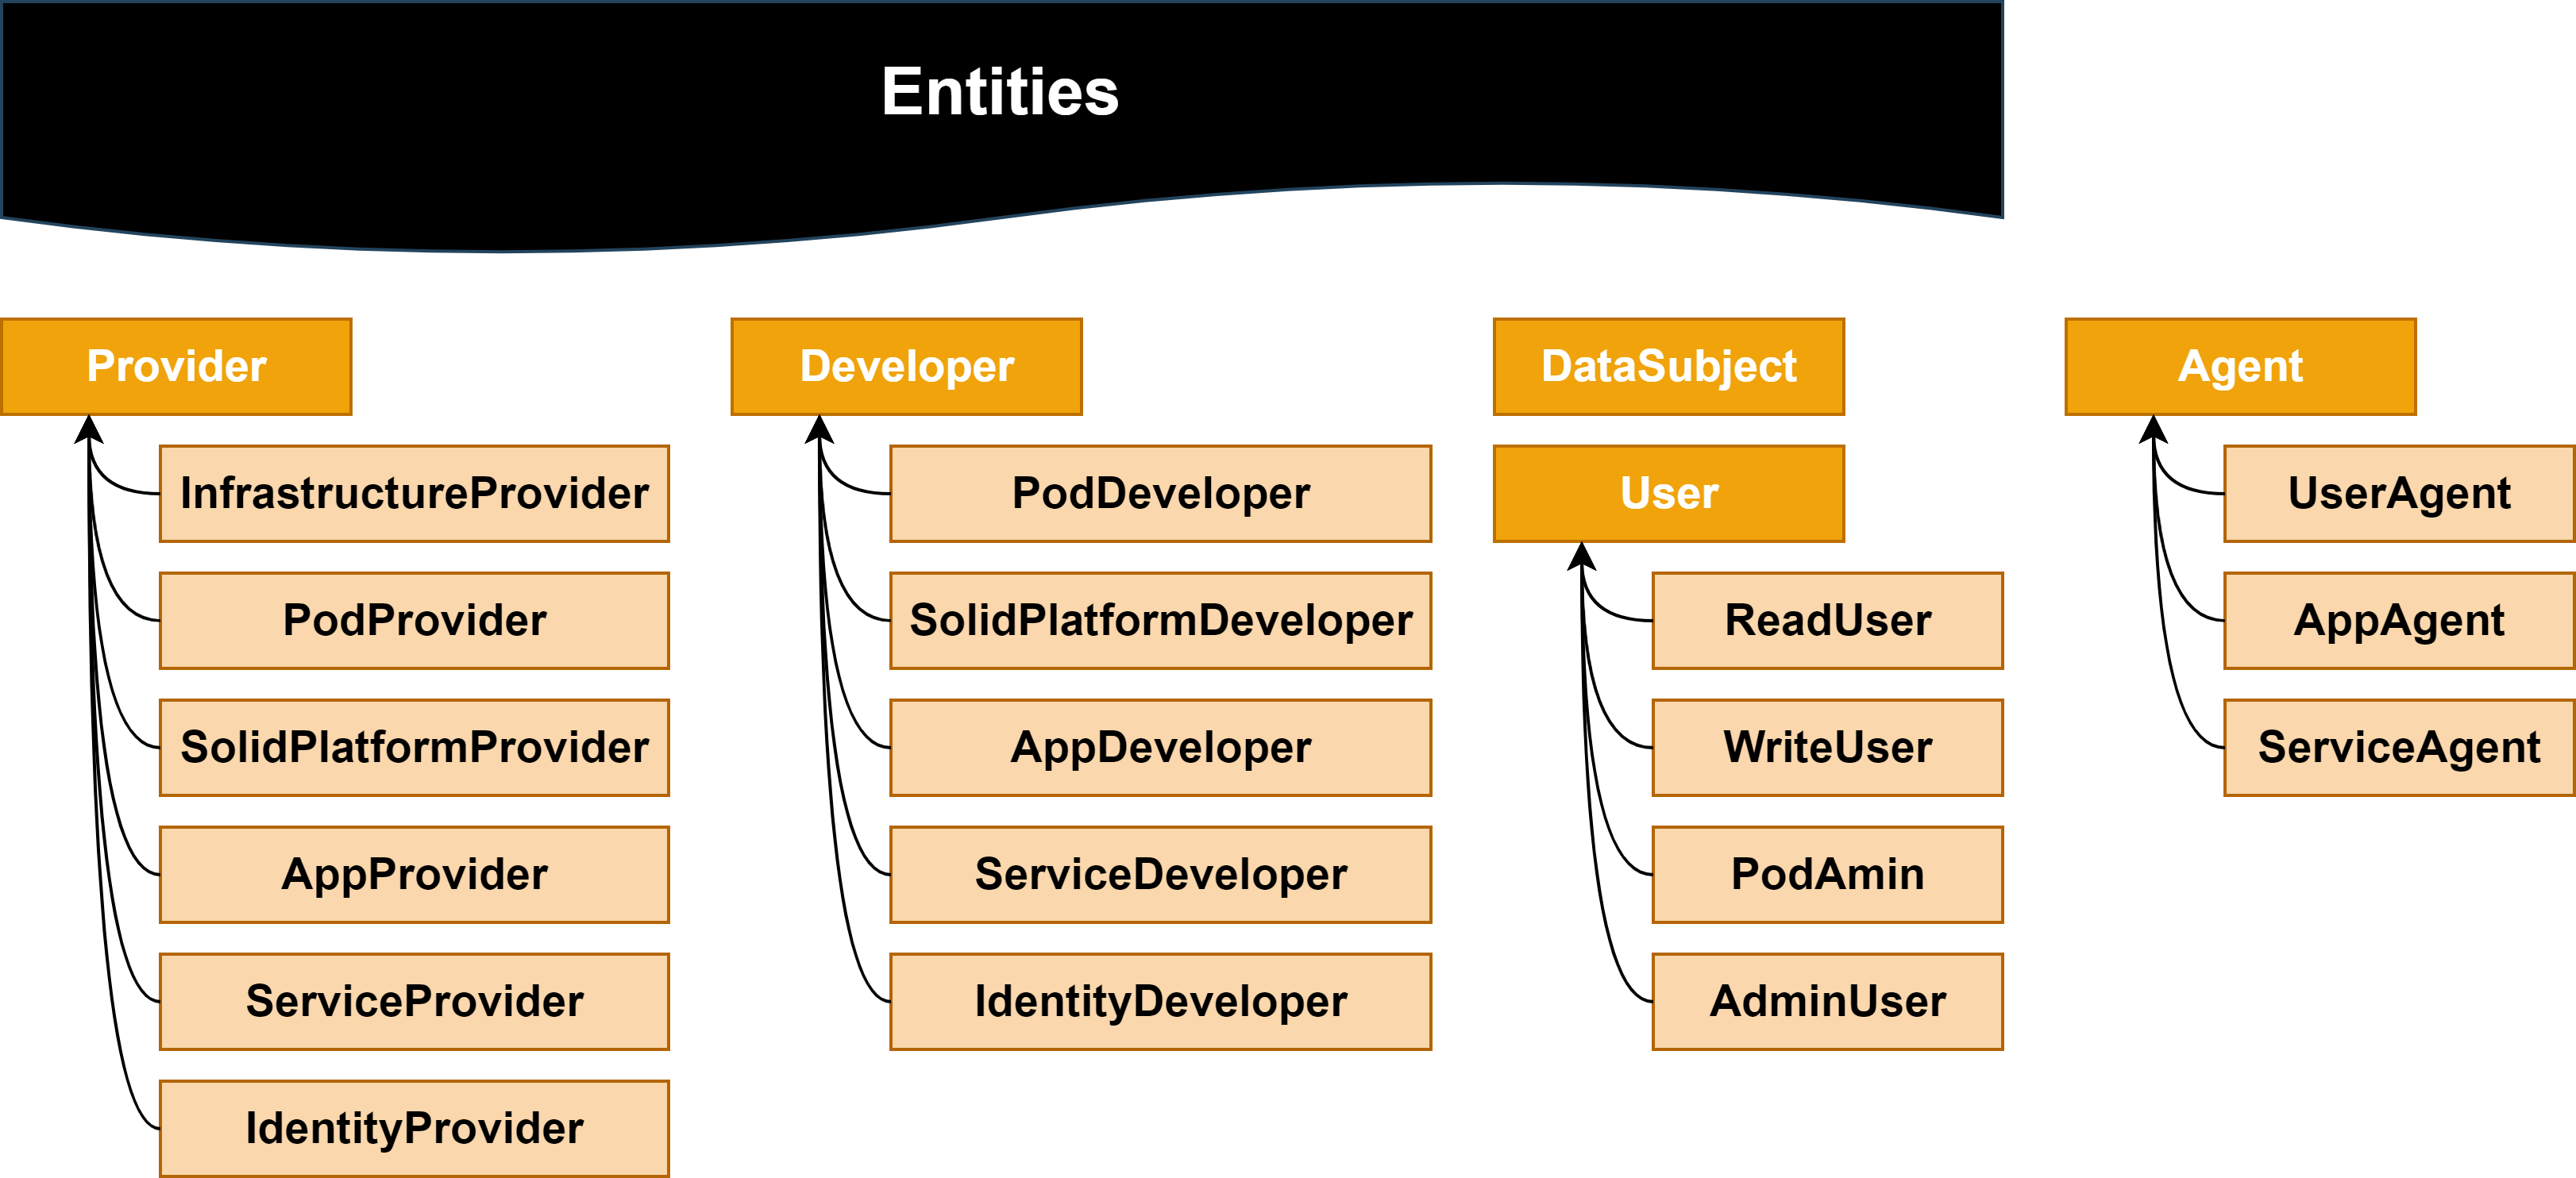
\includegraphics[width=\linewidth]{figures/chapter-4/entities.png}
    \caption{Entities and agents specified in PLASMA.}
    \label{fig:plasma_entities}
\end{figure}

\paragraph{Policies and notices}
In PLASMA, a policy is a document that specifies user, application, and service requirements for data handling practices that apply to data stored or shared through Solid Pods.
Thus, this definition is not limited to access to data stored on a Pod, it also relates to used or transferred data, i.e., to avoid cases such as data collected for purpose X being used for purpose Y.
Such a definition aids with the alignment with legal requirements, e.g., it requires that all purposes must be stated at the time of data collection and that requesters need new consent from the data subject if the purpose for access changes.
PLASMA provides definitions for user policies, in particular for user offers, requirements and preferences, aligned with the \texttt{odrl:Offer}, \texttt{oac:Requirement} and \texttt{oac:Preference} concepts described in Section~\ref{sec:oac}.
Regarding data requests, i.e., conditions for apps and services to have access to or use Pod data, PLASMA envisions their integration into the ecosystem by declaring them in a manifest such as the one being conceived in the W3C Web Application Manifest specification -- an application manifest is a \textit{``JSON document that contains startup parameters and application defaults for when a web application is launched''} \citep{manifest_2023}.
However, the current specification is not enough to achieve legal compliance as it does not include information on entities developing the app, their identity and contact details or their privacy policies.
Thus, PLASMA includes app manifest and service manifest concepts.
In addition to user policies and data requests, PLASMA also provides different types of data agreements, a concept that is completely missing from the Solid specifications as they only provide concepts to refer to apps and users' access authorisations.
As such, an agreement can either be based on the user's consent, or governed by a contract between the user and the entity having responsibility for the app, service or Pod.

Additionally, current Solid specifications also lack the definition of notices.
Notices are documents that provide context information about entities, operations, or data involved in specific processes, e.g., notices may specify the providers, developers, and/or data handling practices of applications and services. 
In this regard, PLASMA provides terms for declaring \textit{ex-ante} and \textit{ex-post} notices, as well as privacy notices for Pods, users, applications and services.

Figure~\ref{fig:plasma_policies} illustrates the policies and notices concepts specified in PLASMA.

\begin{figure}[htb]
    \centering
    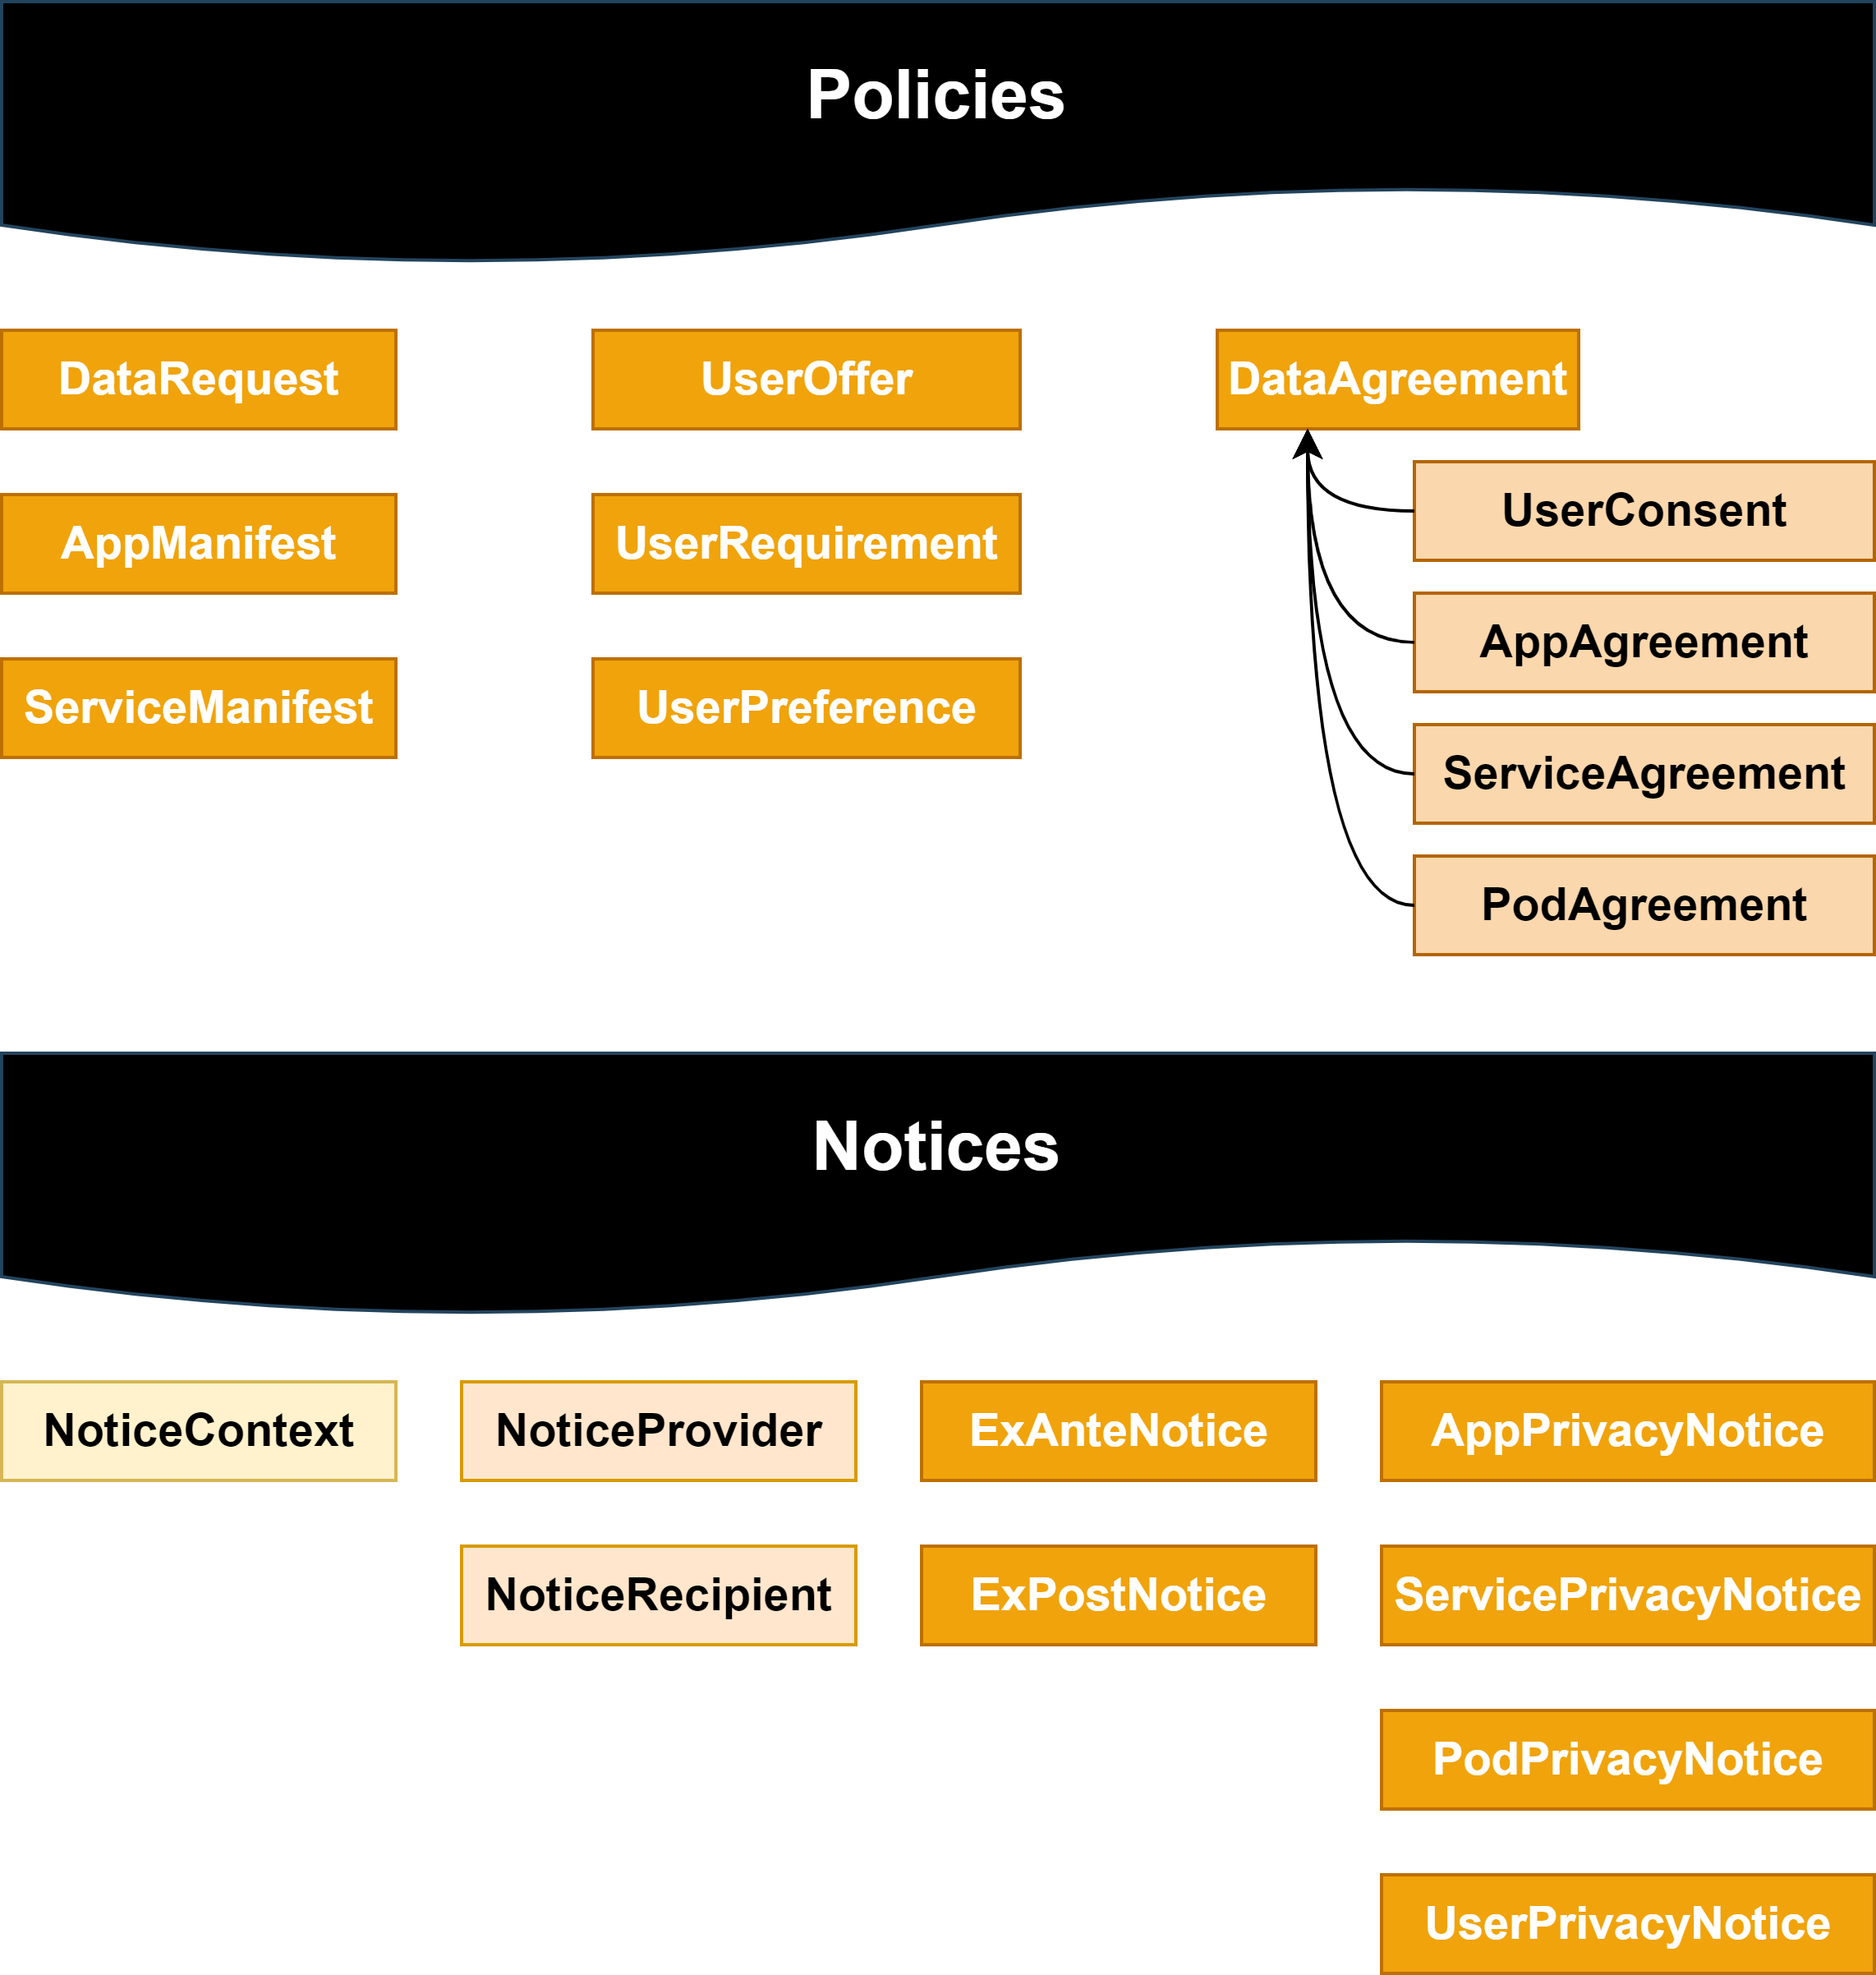
\includegraphics[width=0.8\linewidth]{figures/chapter-4/policies_notices.png}
    \caption{Policy types and notices specified in PLASMA.}
    \label{fig:plasma_policies}
\end{figure}

\paragraph{Services}
PLASMA differentiates between an app and a service -- services convey functionalities that do not need to be packaged as an app.
Moreover, an app requires human intervention to perform some action on data for a specific purpose, while a service may not require human intervention to use or interact with data within a Pod.
Since services are a new concept being introduced by PLASMA in the Solid ecosystem, a taxonomy of twelveu Solid-related services, which can be further expanded, is supplied and illustrated in Figure~\ref{fig:plasma_services}.

\begin{figure}[htb]
    \centering
    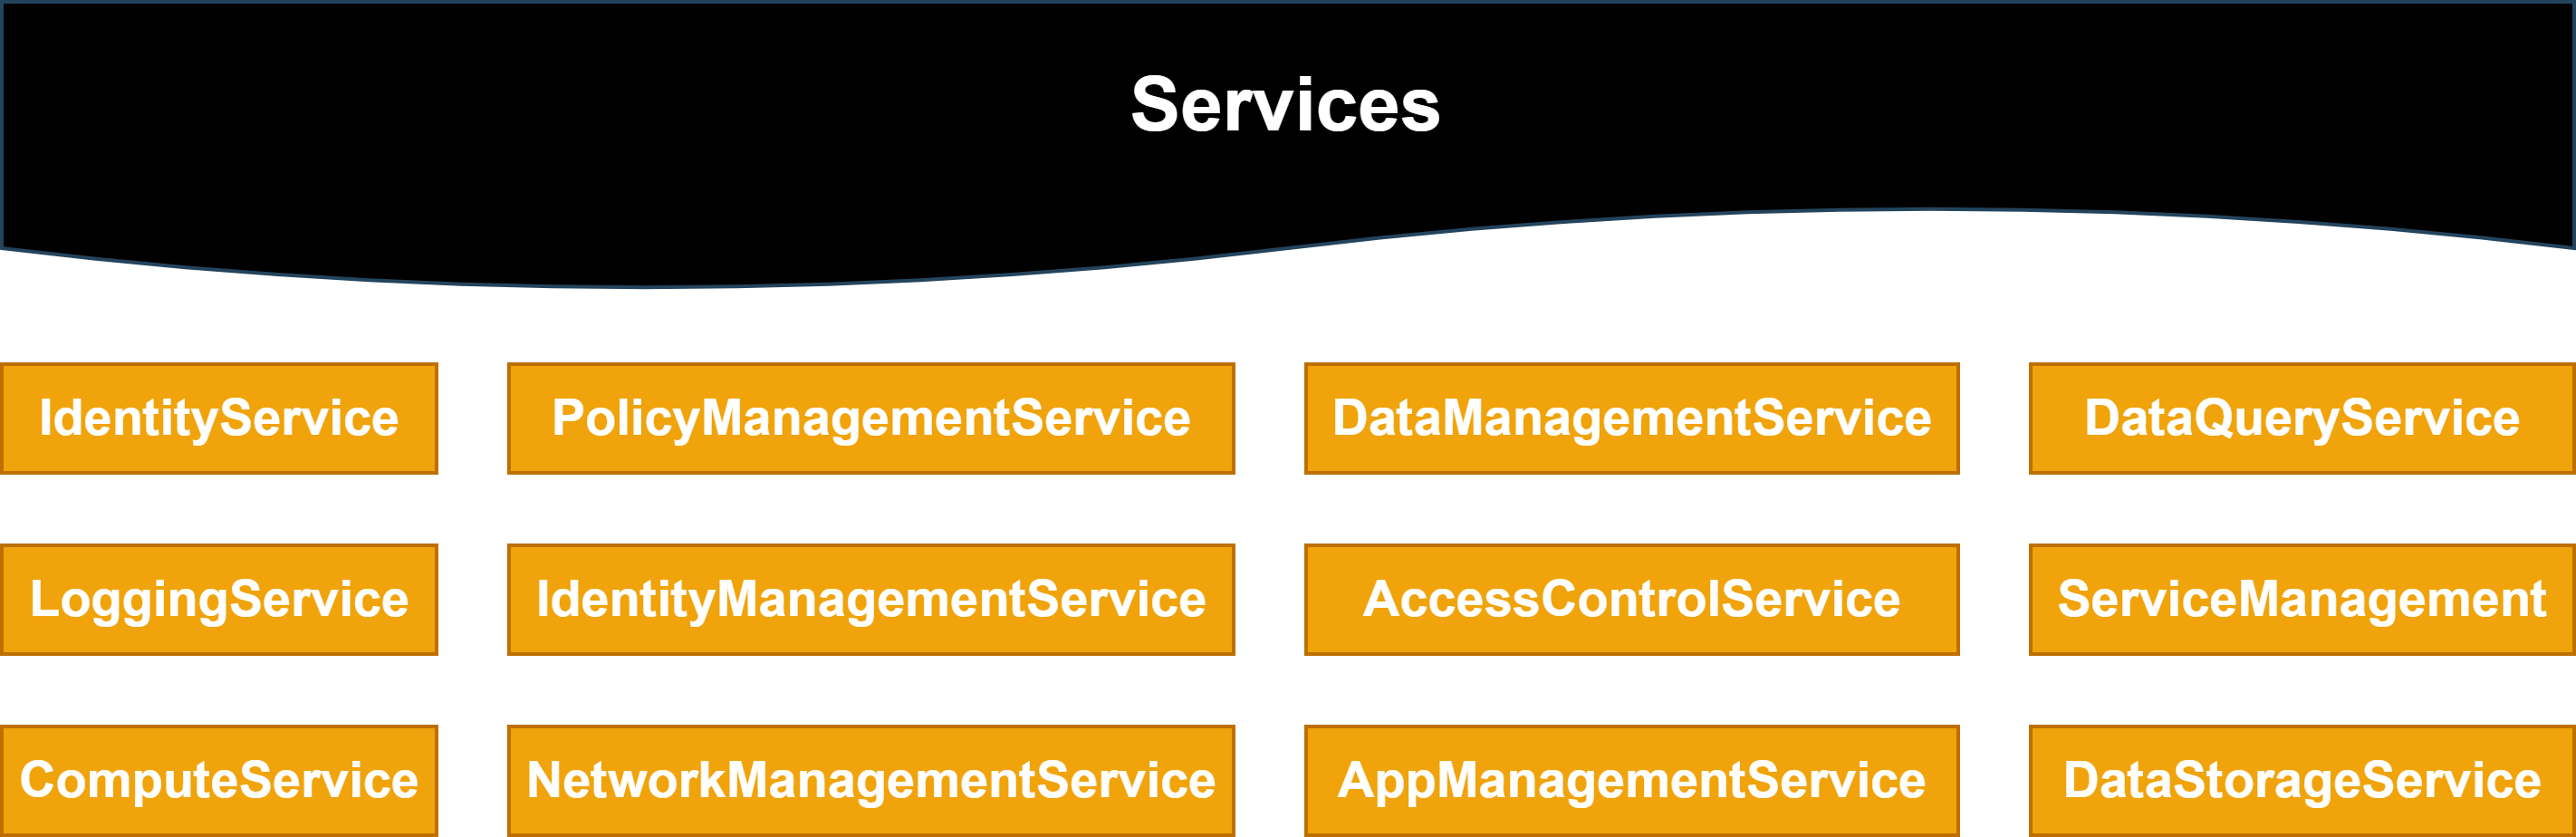
\includegraphics[width=\linewidth]{figures/chapter-4/services.png}
    \caption{Services specified in PLASMA.}
    \label{fig:plasma_services}
\end{figure}

\paragraph{Pod-related data}
To fulfil Solid's vision of providing individuals with a decentralised data storage service for their data and the choice of which applications or services to use for a specific task, metadata regarding Pod management, entities, apps, services, logs and registries should be provided.
Additionally, supervisory authorities can use such logging and provenance metadata, from the Pods of users, for auditing activities, e.g., an EU data protection authority can use these records to investigate a personal data breach.
To this end, PLASMA includes a collection of Solid-related log terms to record provenance information related to processes such as adding or updating resources in a Pod, i.e., a \texttt{DataLog}, registering a policy negotiation procedure reliant on user consent, i.e., a \texttt{PolicyLog}, or recording a successful user login operation, i.e., a \texttt{IdentityLog}.
Furthermore, the maintenance of registries as indexed records for providing collective and convenient access to data within a Pod is of the utmost importance for users, apps and services to have knowledge of the availability of data categories, supported schemas for data, apps, services, relevant policies and users that have/had access to data stored within a Pod.

Figure~\ref{fig:plasma_data} illustrates the Pod-related data concepts defined in PLASMA, including logs and registries.

\begin{figure}[htbp]
    \centering
    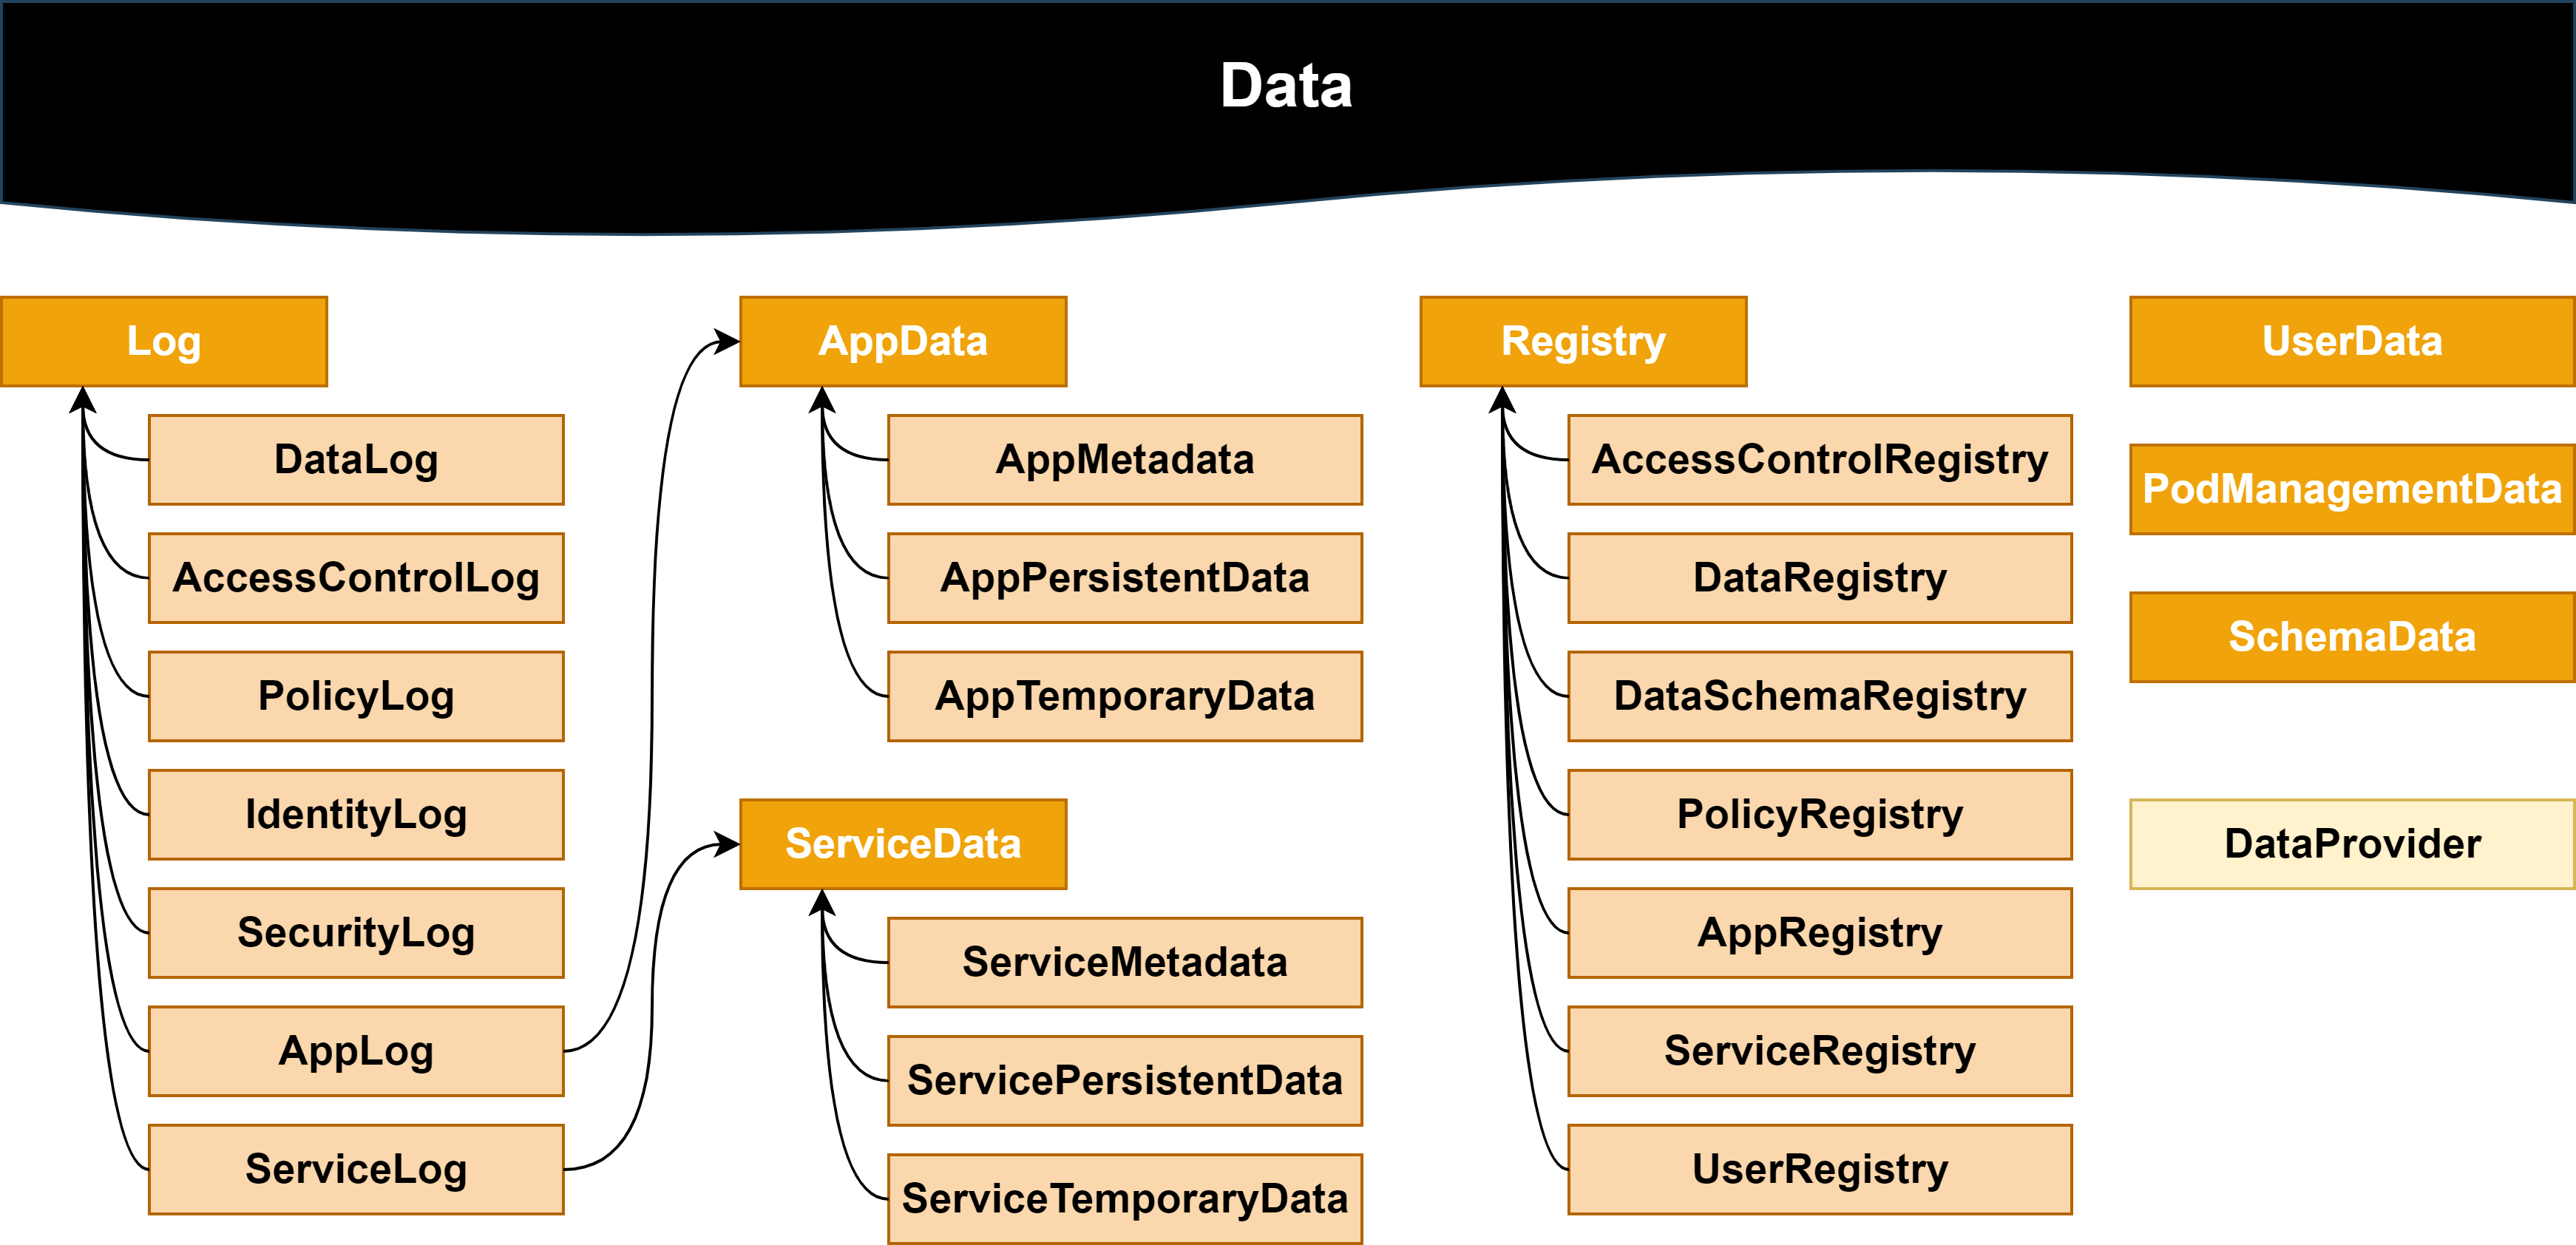
\includegraphics[width=\linewidth]{figures/chapter-4/data.png}
    \caption{Data concepts, including logs and registries, specified in PLASMA.}
    \label{fig:plasma_data}
\end{figure}

\subsection{Conformance with PLASMA}
\label{sec:plasma_conformance}

In this Section, the conditions for Pods, apps, services, users and agents to be conformant with PLASMA are described, including information regarding what is mandatory (indicated below by the use of the word \textit{`must'}) or optional (indicated below by the use of the word \textit{`may'}) to be provided, and how conformity should be evaluated and assured by implementers of the PLASMA specification.

The W3C Recommendation on Data on the Web Best Practices, which is aimed at the \textit{``publication and usage of data on the Web designed to help support a self-sustaining ecosystem''} \citep{loscio_data_2017}, was followed for the publication of metadata related to provenance, licensing and versioning of data.
The vocabulary specifications for particular tasks, recommended by this best practices document, are mentioned in the following paragraphs.

\paragraph{Pod conformance}
For a Pod to be conformant with the PLASMA specification, the following conditions should be satisfied:

\begin{itemize}
    \item A Pod \textit{must} provide or declare \texttt{PodManagementData} which includes metadata about the Pod and of its providers and/or developers, as well as the specific \texttt{SolidPlatform} and \texttt{SolidSpecification} implemented in the Pod and any \texttt{PodAgreement} in place. Listing~\ref{list:plasma_PodManagementData} provides an example of the declaration of such metadata.
    \item A Pod \textit{must} implement or provide equivalent functionality to support the different registries and logs specified in PLASMA. Listing~\ref{list:plasma_dataschemaregistry} provides an example of a data schema registry that records data schemas, formats or shapes recognised or supported by Pods, apps or services, as indicated by the \texttt{plasma:supportedBy} property.
    \item A Pod \textit{may} have multiple users with varying degrees of control. A record of the different users and their level of access \textit{must} be kept in the \texttt{UserRegistry}.
    \item A Pod \textit{may} have discovery methods for users to make their data publicly available.
\end{itemize}

In addition to the ODRL and DCMI Metadata Terms vocabularies, the DPV's \texttt{hasName}, \texttt{hasContact} and \texttt{hasAddress} properties should be used to identify and provide contact details of the Pod, Solid platform and infrastructure providers and developers. \textit{Schema.org} and the Provenance, Authoring and Versioning (PAV) vocabularies, along with the previously mentioned DCMI, are used to describe the authors, sources, version and code repository URIs of the platform and specification installed within the Pod. \textit{Schema.org} provides an upper vocabulary of terms to describe \textit{``entities, relationships between entities and actions''} related to structured data on the Web \citep{guha_schemaorg_2015} and PAV is a \textit{``lightweight ontology for tracking Provenance, Authoring and Versioning''} that \textit{``specializes the W3C provenance ontology PROV-O in order to describe authorship, curation and digital creation of online resources''} \citep{ciccarese_pav_2013}.

\begin{listing}[htp]
\caption{Metadata of Beatriz's Pod.}
\label{list:plasma_PodManagementData}
\begin{minted}{turtle}
<https://solidweb.me/besteves4/PodMetadata> a plasma:PodManagementData ;
    dcterms:description "Metadata of Beatriz's Pod" ;
    odrl:hasPolicy <https://solidweb.me/besteves4/agreements/Pod> ;
    plasma:hasProvider <https://solidweb.me/besteves4/entities/PodProvider> ;
    plasma:hasProvider <https://solidweb.me/besteves4/entities/PlatformProvider> ;
    plasma:hasProvider <https://solidweb.me/besteves4/entities/InfrastructureProvider> ;
    plasma:implementedSolidPlatform <https://solidweb.me/besteves4/Platform> ;
    plasma:implementedSolidSpecification <https://solidweb.me/besteves4/SolidSpec> .

<https://solidweb.me/besteves4/agreements/Pod> a plasma:PodAgreement .

<https://solidweb.me/besteves4/entities/PodProvider> a plasma:PodProvider ;
    dpv:hasName "Entity A" ; dpv:hasContact "mailto:entity_a@mail.com" ;
    dpv:hasAddress "Address of Entity A" .

<https://solidweb.me/besteves4/entities/PlatformProvider> a plasma:SolidPlatformProvider .

<https://solidweb.me/besteves4/entities/InfrastructureProvider> a plasma:InfrastructureProvider .

<https://solidweb.me/besteves4/Platform> a plasma:SolidPlatform ;
    plasma:hasProvider <https://solidweb.me/besteves4/entities/PlatformProvider> ;
    dcterms:source <https://communitysolidserver.github.io> ;
    dpv:hasPolicy <https://www.serverproject.de/files/solidweb_me_terms.txt> ;
    schema:codeRepository <https://github.com/CommunitySolidServer/CommunitySolidServer> ;
    pav:version "6.1.0" ;
    dcterms:license <https://dalicc.net/licenselibrary/MIT> .

<https://solidweb.me/besteves4/SolidSpec> a plasma:SolidSpecification ;
    dcterms:conformsTo <https://solidproject.org/TR/2022/protocol-20221231> ;
    dcterms:creator "Sarven Capadisli", "Tim Berners-Lee", "Ruben Verborgh", "Kjetil Kjernsmo" ;
    dcterms:license <https://dalicc.net/licenselibrary/MIT> ;
    pav:version "0.10.0" ; dcterms:created "2022-12-31"^^xsd:date ;
    schema:codeRepository <https://github.com/solid/specification> .
\end{minted}
\end{listing}

\begin{listing}[htp]
\caption{Data schema registry of Beatriz's Pod.}
\label{list:plasma_dataschemaregistry}
\begin{minted}{turtle}
<https://solidweb.me/besteves4/SchemaRegistry> a plasma:DataSchemaRegistry ;
    dcterms:description "Registry listing recognised or supported schemas" ;
    dcterms:created "2023-09-10T11:51:17"^^xsd:dateTime ;
    dcterms:modified "2023-10-07T12:39:50"^^xsd:dateTime ;
    dcterms:publisher <https://solidweb.me/besteves4/entities/DataMgtServiceProvider> ;
    plasma:hasSchema <https://solidweb.me/besteves4/schemas/EHR-schema>,
        <https://solidweb.me/besteves4/schemas/img-format>,
        <https://solidweb.me/besteves4/schemas/entity-shape> .

<https://solidweb.me/besteves4/entities/DataMgtServiceProvider> a plasma:ServiceProvider ;
    plasma:serviceType plasma:DataManagementService ;
    dpv:hasName "Entity A" ;
    dpv:hasAddress "Address of Entity A" ;
    dpv:hasContact "mailto:entity_a@mail.com" .

<https://solidweb.me/besteves4/schemas/EHR-schema> a plasma:SchemaData ;
    dcterms:conformsTo <http://www.w3.org/TR/turtle/> ;
    plasma:supportedBy <https://example.com/health-service> .

<https://example.com/health-service> a plasma:Service .

<https://solidweb.me/besteves4/schemas/img-format> a plasma:SchemaData ;
    dcterms:format <https://www.iana.org/assignments/media-types/image/png>,
        <https://www.iana.org/assignments/media-types/image/svg+xml> ;
    plasma:supportedBy <https://example.com/social-app> .

<https://example.com/social-app> a plasma:App .

<https://solidweb.me/besteves4/schemas/entity-shape> a plasma:SchemaData, sh:NodeShape ;
    plasma:supportedBy <https://solidweb.me/besteves4/> ;
    sh:name "PLASMA entity shape" ;
    sh:description "Minimum data that PLASMA entities should provide to be identified." ;
    sh:targetClass plasma:Entity .
\end{minted}
\end{listing}

% software description: https://w3id.org/okn/o/sd
% paper: Towards Assessing FAIR Research Software Best Practices in an Organization Using RDF-star. Ana Iglesias-Molina and Daniel Garijo

\paragraph{Apps and services conformance}
For an app or service to be conformant with the PLASMA specification, the following conditions should be satisfied:

\begin{itemize}
    \item An app, or service, \textit{must} have an \texttt{AppManifest}, or \texttt{ServiceManifest}, in conformance with the W3C Web Application Manifest \citep{manifest_2023}. A Pod \textit{may} ensure manifest conformance using SHACL shapes. Listing~\ref{list:plasma_appmanifest} provides an example of an app manifest.
    \item An \texttt{AppManifest}, or \texttt{ServiceManifest}, \textit{must} include information regarding the developer and provider of legally relevant entities and their identities.
    \item An \texttt{AppManifest}, or \texttt{ServiceManifest}, \textit{must} state the \texttt{DataRequest} representing the request to use data using the \texttt{odrl:hasPolicy} property. The request \textit{must} provide all information regarding the use of data even if only some of it will be applicable initially or used in the notice.
    \item An \texttt{AppManifest}, or \texttt{ServiceManifest}, \textit{must} link the privacy notice of the app, or service, using the \texttt{dpv:hasNotice} property. The Pod \textit{may} use this information to display or optionally construct its own notice based on the preferences or accessibility requirements of the user.
    \item An \texttt{AppManifest}, or \texttt{ServiceManifest}, \textit{must} be stored in the Pod \texttt{AppRegistry}, or \texttt{ServiceRegistry}. Listing~\ref{list:plasma_appregistry} provides an example of an app registry, where app-related metadata, including the manifest, app providers and developers, temporary or persistent app data, is recorded.
    \item Apps, or services, \textit{may} have multiple \texttt{AppAgents}, or \texttt{ServiceAgents}, which \textit{must} be registered in the \texttt{AppRegistry}, or \texttt{ServiceRegistry}.
\end{itemize}

In addition to the PLASMA terms mentioned in the previous list, the usage of the \texttt{plasma:serviceType} property can be used to connect service providers and developers with a particular type of service, e.g., from PLASMA's service taxonomy, that is provided or developed by said entity.
Moreover, it should be noted that app or service stores, such as those maintained by Apple and Google, can also act as app or service providers and the FOAF \texttt{page} property can be used to actually connect the store provider with the store itself.
The FOAF vocabulary specification \citep{brickley_foaf_2004} provides terms to describe people and related personal information and online accounts.
Regardless, support for other optional properties specified in the W3C Web Application Manifest specification, such as icons, display mode, orientation, and background colour, can also be integrated into the modelled manifests, as well as `common' app store metadata, such as screenshots, user rating or app type, e.g., health, game or news app \citep{gustafson_web_2023}.

\begin{listing}[htp]
\caption{App manifest of Contacts app.}
\label{list:plasma_appmanifest}
\begin{minted}{turtle}
<https://example.com/Contacts> a plasma:App ;
    plasma:hasAppManifest <https://example.com/Contacts/Manifest> .

<https://example.com/Contacts/Manifest> a plasma:AppManifest ;
    dcterms:conformsTo <https://www.w3.org/TR/appmanifest/> ;
    dcterms:issued "2023-10-23T22:43:58"^^xsd:dateTime ;
    dcterms:title "Contacts" ;
    dcterms:description "App to manage contacts" ;
    dcterms:language <http://id.loc.gov/vocabulary/iso639-1/en> ;
    plasma:hasProvider <https://solidweb.me/besteves4/entities/AppStore> ;
    plasma:hasDeveloper <https://solidweb.me/besteves4/entities/ContactsDeveloper> ;
    odrl:hasPolicy <https://example.com/Contacts/Request> ;
    dpv:hasNotice <https://example.com/Contacts/Notice> .

<https://solidweb.me/besteves4/entities/AppStore> a plasma:AppProvider ;
    dpv:hasName "App Store provider" ;
    dpv:hasAddress "Address of App Store provider" ;
    dpv:hasContact "mailto:app_store@mail.com" ;
    foaf:page <https://example.com/AppStore> ;
    dpv:hasNotice <https://example.com/AppStore/PrivacyPolicy> .

<https://solidweb.me/besteves4/entities/ContactsDeveloper> a plasma:AppDeveloper .

<https://example.com/Contacts/request> a plasma:DataRequest, odrl:Request .
\end{minted}
\end{listing}

\begin{listing}[htp]
\caption{App registry of Beatriz's Pod.}
\label{list:plasma_appregistry}
\begin{minted}{turtle}
<https://solidweb.me/besteves4/AppRegistry> a plasma:AppRegistry ;
    dcterms:description "Registry listing apps" ;
    dcterms:created "2023-09-30T11:33:35"^^xsd:dateTime ;
    dcterms:modified "2023-10-07T11:31:40"^^xsd:dateTime ;
    dcterms:publisher <https://solidweb.me/besteves4/entities/AppMgProvider> ;
    plasma:hasApp <https://solidweb.me/besteves4/apps/Contacts/> .

<https://solidweb.me/besteves4/entities/AppMgProvider> a plasma:ServiceProvider ;
    plasma:serviceType plasma:AppManagementService .

<https://solidweb.me/besteves4/apps/Contacts/> a plasma:App ;
    plasma:hasAppManifest <https://solidweb.me/besteves4/apps/Contacts/Manifest> ;
    odrl:hasPolicy <https://solidweb.me/besteves4/apps/Contacts/Agreement> ;
    plasma:hasAppMetadata <https://solidweb.me/besteves4/apps/Contacts/Metadata> ;
    plasma:hasAppPersistentData <https://solidweb.me/besteves4/apps/Contacts/PersistentData> ;
    plasma:hasAppTemporaryData <https://solidweb.me/besteves4/apps/Contacts/TemporaryData> ;
    plasma:hasAgent <https://solidweb.me/besteves4/apps/Contacts/Agent> .

<https://solidweb.me/besteves4/apps/Contacts/Metadata> a plasma:AppMetadata ;
    dcterms:description "Contacts metadata" ;
    plasma:hasProvider <https://solidweb.me/besteves4/entities/AppStore> ;
    plasma:hasDeveloper <https://solidweb.me/besteves4/entities/ContactsDeveloper> .

<https://solidweb.me/besteves4/apps/Contacts/PersistentData> a plasma:AppPersistentData ;
    dcterms:type dpv-pd:TelephoneNumber ; rdf:value "(+34)691485135" .

<https://solidweb.me/besteves4/apps/Contacts/TemporaryData> a plasma:AppTemporaryData ;
    dcterms:type dpv-pd:TelephoneNumber ; rdf:value "(+34)691998745" ;
    dcterms:valid "2023-10-01T14:50:21"^^xsd:dateTime .

<https://solidweb.me/besteves4/apps/Contacts/Agent> a plasma:AppAgent .
\end{minted}
\end{listing}

\paragraph{User conformance}
For a user to be conformant with the PLASMA specification, the following conditions should be satisfied:

\begin{itemize}
    \item Impactful interactions of a user, e.g., changing identity providers, \textit{must} be recorded using a well-defined shape. Listing~\ref{list:plasma_accesscontrollog} provides an example of access control logs modelled with PLASMA and using W3C's Activity Streams activity types \citep{snell_activity_2017}.
    \item A \texttt{UserRegistry} \textit{must} contain information regarding the \texttt{DataSubjects} storing data within a Pod, the \texttt{PodAdmin} and other users accessing Data. Listing~\ref{list:plasma_userregistry} provides an example of said registry.
    \item Users \textit{may} be directly associated with a \texttt{DataRequest} so that they can make requests for data without using an application or service.
    \item Users \textit{may} have multiple \texttt{UserAgents}, which should be registered in the \texttt{UserRegistry}.
\end{itemize}

PLASMA recommends the usage of the W3C's Activity Streams vocabulary \citep{snell_activity_2017} to model the distinct logs that should be stored in Solid Pods for transparency and accountability, e.g., data, identity or policy logs.
This recommendation provides an extensive list of activity, actor and object types that provides ``a baseline extensible syntax for the expression of completed activities''.
Such syntax allows the identification of the resource being logged, using the \texttt{as:object} property, the entity responsible for the activity being logged, using the \texttt{as:actor} property, or the app or service used to generate the log, employing the \texttt{as:generator} property.
The \texttt{as:Accept} and \texttt{as:Reject} activity types can be reused to express when access to data or policies are accepted or rejected, and the \texttt{as:Create}, \texttt{as:Update}, \texttt{as:Delete} and \texttt{as:Move} activities can be reused to log the creation, modification, deletion or movement of data or policies.
New activity types, e.g., to request data, change identity providers or verify the identity of apps, which are not modelled by the Activity Streams vocabulary, are modelled in PLASMA, e.g., as \texttt{plasma:Request}, \texttt{plasma:ChangeIdP} or \texttt{plasma:Verify}.

It should also be stated that Inrupt's Enterprise Solid Server has started to provide an auditing service\footnote{\url{https://docs.inrupt.com/ess/latest/services/service-auditing/} (accessed on 21 December 2023)} which also relies on the W3C Activity Streams 2.0 Recommendation \citep{snell_activity_2017} to document audit events related with the identity of user and applications.

\begin{listing}[htp]
\caption{Access control logs recorded in Beatriz's Pod.}
\label{list:plasma_accesscontrollog}
\begin{minted}{turtle}
<https://solidweb.me/besteves4/logs/AccessControl_Reject> a plasma:AccessControlLog ;
	dcterms:type as:Reject ;
	dcterms:issued "2023-11-12T15:34:04"^^xsd:dateTime ;
	as:summary "Access to data rejected" ;
	as:object <https://solidweb.me/besteves4/health/ehr> ;
	as:actor <https://solidweb.me/arya/profile/card#me> ;
	as:generator <https://example.com/App> ;
	dcterms:publisher <https://solidweb.me/besteves4/entities/LoggingProvider> .

<https://solidweb.me/besteves4/logs/AccessControl_Accept> a plasma:AccessControlLog ;
	dcterms:type as:Accept ;
	dcterms:issued "2023-11-12T15:43:09"^^xsd:dateTime ;
	as:summary "Access to data accepted" ;
	as:object <https://solidweb.me/besteves4/contacts/> ;
	as:actor <https://solidweb.me/arya/profile/card#me> ;
	as:generator <https://example.com/App> ;
	dcterms:publisher <https://solidweb.me/besteves4/entities/LoggingProvider> .

<https://example.com/App> a plasma:App .

<https://solidweb.me/besteves4/entities/LoggingProvider> a plasma:ServiceProvider ;
	plasma:serviceType plasma:LoggingService ;
	dpv:hasName "Entity G" ;
	dpv:hasAddress "Address of Entity G" ;
	dpv:hasContact "mailto:entity_g@mail.com" .
\end{minted}
\end{listing}

\begin{listing}[htp]
\caption{User registry of Beatriz's Pod.}
\label{list:plasma_userregistry}
\begin{minted}{turtle}
<https://solidweb.me/besteves4/UserRegistry> a plasma:UserRegistry ;
    dcterms:description "Registry listing users" ;
    dcterms:created "2023-09-30T11:33:35"^^xsd:dateTime ;
    dcterms:modified "2023-10-07T12:39:50"^^xsd:dateTime ;
    dcterms:publisher <https://solidweb.me/besteves4/entities/UserMProvider> ;
    dpv:hasDataSubject <https://solidweb.me/besteves4/entities/DataSubject> ;
    plasma:hasUser <https://solidweb.me/besteves4/entities/DataSubject>,
        <https://solidweb.me/besteves4/entities/ReadUserA>,
        <https://solidweb.me/besteves4/entities/ReadUserB>,
        <https://solidweb.me/besteves4/entities/Admin> .

<https://solidweb.me/besteves4/entities/UserMProvider> a plasma:ServiceProvider ;
    dpv:hasName "Entity A" ;
    dpv:hasAddress "Address of Entity A" ;
    dpv:hasContact "mailto:entity_a@mail.com" .

<https://solidweb.me/besteves4/entities/DataSubject> a plasma:DataSubject, plasma:PodAdmin ;
    dpv:hasName "Data Subject" ;
    dpv:hasAddress "Address of Data Subject" ;
    dpv:hasContact "mailto:data_subject@mail.com" ;
    plasma:hasAgent <https://solidweb.me/besteves4/agents/AgentA> .

<https://solidweb.me/besteves4/agents/AgentA> a plasma:UserAgent .

<https://solidweb.me/besteves4/entities/ReadUserA> a plasma:ReadUser ;
    plasma:hasPolicy <https://solidweb.me/besteves4/requests/UserA> .

<https://solidweb.me/besteves4/entities/UserA> a plasma:DataRequest .

<https://solidweb.me/besteves4/entities/ReadUserB> a plasma:ReadUser ;
    plasma:hasPolicy <https://solidweb.me/besteves4/requests/UserB> ;
    plasma:hasPolicy <https://solidweb.me/besteves4/agreements/UserB> .

<https://solidweb.me/besteves4/agreements/UserB> a odrl:Agreement, plasma:UserConsent .

<https://solidweb.me/besteves4/entities/Admin> a plasma:AdminUser .
\end{minted}
\end{listing}

\paragraph{Agent conformance}
For an agent to be conformant with the PLASMA specification, the following conditions should be satisfied:

\begin{itemize}
    \item Agents activity \textit{must} be in accordance with the manifest of the entity for which they are acting on behalf of.
    \item A record of the usage of an \texttt{AppAgent}, \texttt{ServiceAgent} or \texttt{UserAgent} \textit{must} be kept in the \texttt{AppRegistry}, \texttt{ServiceRegistry} or \texttt{UserRegistry}, respectively, including information regarding its providers/developers for accountability. User \url{https://solidweb.me/besteves4/entities/DataSubject} in Listing~\ref{list:plasma_userregistry} has a user agent identified with the PLASMA property \texttt{hasAgent}.
\end{itemize}

Finally, each of the requirements established in the previous paragraphs for the conformance of Pods, apps, services, users and agents with PLASMA should be verified using a language for describing and validating RDF graphs.
As such, SHACL can, not only, be used for the definition of data shapes recognised or supported by apps, services or Pods, but also can act as a general tool to verify conformance with the conditions specified in this Section.
SHACL was chosen for this conformance checking since it is a widely used and supported W3C Recommendation for \textit{``validating RDF graphs against a set of conditions''} \citep{knublauch_shapes_2017}.
SHACL shapes for all the previously mentioned conformance conditions were generated in this Thesis and are provided in the Appendix.

% SHACL shapes generator: https://github.com/AKSW/shaclgen

% PLASMA is available at \url{https://w3id.org/plasma}, under the CC-By-4.0 license, and reuses the available terms in the Solid vocabularies, when appropriate, in line with FAIR (Findable, Accessible, Interoperable, Reusable) principles. Each taxonomy is discussed below.

% Externally, `app stores' such as those maintained by Apple and Google and `package repositories' such as those maintained by Linux distributions also feature the use of metadata that developers must provide in order for their apps to be enlisted in their stores. These platforms also use this metadata for governing apps, identifying compatibility, and enforcing guidelines.

\subsection{Vocabulary publication and maintenance}
\label{sec:plasma_publication}

The vocabulary human-readable documentation and machine-readable file are available at \url{https://w3id.org/plasma} using content negotiation.
The HTML documentation includes a description of the terms defined in PLASMA, which was conducted and validated with domain experts, diagrams with graphical representations of the several taxonomies included in the vocabulary, a detailed explanation of the conformance conditions that need to be adopted by Pods, apps, services, agents and users for them to be PLASMA-compliant, RDF examples of workflows that use PLASMA terms for specific scenarios, e.g., creating user policies or auditing Pods, and information related to legal compliance.
The vocabulary documentation also includes metadata, such as the identity of the creators and publishers of the ontology, the dates of creation and last modification or the version number.

The source code is hosted at \url{https://w3id.org/plasma/repo}, under the CC-BY-4.0 license.
The repository can also be used by PLASMA implementers to suggest new inclusions to the vocabulary and to report bugs through GitHub Issues.
\section{Exercising data subject rights with DPV}
\label{sec:rights_exercising}

This Section describes the usage of vocabulary-based patterns to describe rights exercising metadata.
Such patterns can be used by entities dealing with the handling of personal data to maintain consistent records of data subject rights exercising activities, aligned with GDPR requirements.
In a decentralised data system environment, these rights must also be fulfilled by data controllers, while notices and records of rights exercising activities can be kept by data subjects in their personal datastores for transparency and accountability.

\subsection{Requirements to express rights-related activities}
\label{sec:rights_concepts}

This Section outlines the motivation and identified requirements for the expression of information related to the exercising of data subject rights.
This work was developed (and is already integrated) within the context of the DPVCG and was started with the main objectives of indicating (i) what rights exist (in particular within the framework of the GDPR), (ii) where such rights can be exercised, and (iii) what information needs to be recorded and maintained when a concrete instance of a right is being/was exercised.

As previously mentioned in Section~\ref{sec:def_gdpr} and represented in Figure~\ref{fig:gdpr_information_flows}, the focus of this Thesis is on the representation of information related to legislation on data protection in the European Union, in particular regarding the GDPR and related data subject rights, listed on Chapter III.
Moreover, in Section~\ref{sec:sota_vocabularies_criteria}, and in particular in Table~\ref{tab:GDPR_privacy_terms}, the privacy terms that need to be represented for such rights to be exercised by data subjects and fulfilled by data controllers.

Figure~\ref{fig:gdpr-rights} illustrates the flows of information between a data subject and a data controller for the exercising of a right request, according to the GDPR.
After sending a notice to the data subject confirming that the request was received, the controller must be able to identify the data subject in order to proceed with the request~(Article 12.2, second sentence~\citeyearpar{noauthor_regulation_2016}).
If the controller cannot identify the data subject, then the data subject must provide additional information to enable the controller to identify them~(Article 11.2~\citeyearpar{noauthor_regulation_2016}).
If the controller disregards the request or has a justification for not fulfilling the right, then the data subject does not receive any information related to the right request~(Article 12.2, second sentence~\citeyearpar{noauthor_regulation_2016}).
In case the controller has a justification to delay the request due to its complexity or a high number of requests, then the controller has a 2-month extension to fulfil its duty~(Article 12.3,
second sentence~\citeyearpar{noauthor_regulation_2016}).
Moreover, in case the request is unfounded or excessive, the controller can charge a fee and the data subject will get the information once this fee is paid~(Article 12.5, first sentence~\citeyearpar{noauthor_regulation_2016}).
As it is visible by the diagram, at any point if the data controller does not fulfil its duty then a GDPR breach occurs and the data subject does not receive their requested information.

% this could be clearer as a uml process diagram with separate swim lanes for subject and controller to clarify which does which activities and decision and also to clarify the start and end states of the flow.
\begin{figure}[htp]
    \centering
    \includegraphics[width=0.78\linewidth]{figures/chapter-4/GDPR-DSR.png}
    \caption[Flow diagram of GDPR data subject rights exercising.]{Flow diagram of GDPR data subject rights exercising, according to Article 12.}
    \label{fig:gdpr-rights}
\end{figure}

From the analysis of these flows of information, a set of high-level concepts was proposed and adopted by the DPVCG (general concepts on Rights are modelled in the main DPV specification at \url{https://w3id.org/dpv#vocab-rights} and GDPR-specific ones in the DPV-GDPR extension at \url{https://w3id.org/dpv/legal/eu/gdpr#vocab-rights}\footnote{The concepts that have `Beatriz Esteves' has a contributor are an outcome of this Thesis}).
Figure~\ref{fig:rights_dpv}, adapted from \cite{pandit_primer_2022}, provides an overview of these concepts.

\begin{figure}[ht]
    \centering
    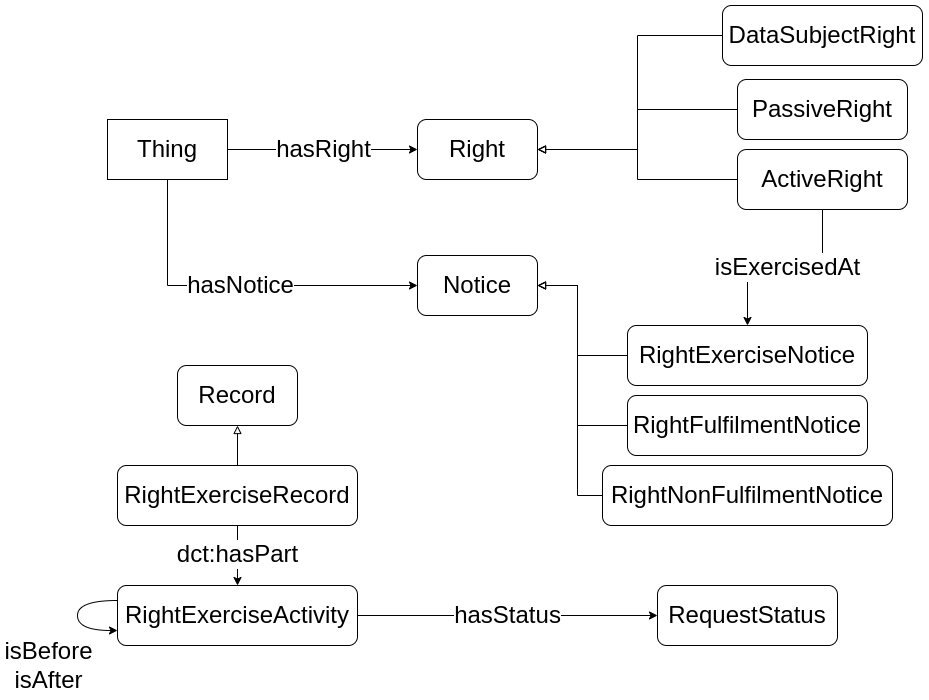
\includegraphics[width=0.8\linewidth]{figures/chapter-4/DPV-rights.png}
    \caption[Core concepts of DPV's rights taxonomy.]{Core concepts of DPV's rights taxonomy, adapted from \cite{pandit_primer_2022}.}
    \label{fig:rights_dpv}
\end{figure}

Thus, beyond modelling concepts for applicable \texttt{Right}s and \texttt{DataSubjectRight}s (applicable only to data subjects), to indicate the association of concepts with a particular right, the \texttt{hasRight} property is also modelled in DPV.
Additionally, to make a distinction between actionable and non-actionable rights, the \texttt{ActiveRight} and \texttt{PassiveRight} concepts were created to distinguish between rights that require an action to be taken for them to be exercised and rights that don't require any action and are always applicable.% add examples of active/passive rights
To fulfil the second objective of establishing where such active rights can be exercised, DPV's \texttt{isExercisedAt} property should be used to connect the right with the \texttt{RightExerciseNotice}.
This notice provides contextual information regarding how to exercise a right.
Specialised notice concepts for rights that can be fulfilled and those that cannot are modelled as \texttt{RightFulfilmentNotice} and \texttt{RightNonFulfilmentNotice}, respectively.

Moreover, to represent concrete records of rights being exercised, the \texttt{RightExerciseRecord} concept, specified as a subclass of DPV's \texttt{Record}, can be used to associate a particular request, or even distinct requests from the same data subject, with corresponding rights exercising activities, modelled as \texttt{RightExerciseActivity}, using the DCMI Metadata Terms \texttt{hasPart} property.
Such activity instances should include metadata, e.g., timestamps, duration, or involved entities, to track the provenance of a particular right exercising process, from the request itself to its acknowledgement by the data controller and to the fulfilment or non-fulfilment of the right.

In order to justify a certain right exercise activity, a collection of justifications for the non-fulfilment, i.e., \texttt{RightNonFulfilmentJustification}, delay of fulfilment, i.e.,\linebreak \texttt{RightFulfilmentDelayJustification}, and exercise of rights, i.e.,\linebreak \texttt{RightExerciseJustification}, were modelled as subclasses of the\linebreak \texttt{NonPerformanceJustification}, \texttt{DelayJustification}, and\linebreak \texttt{ExerciseJustification} concepts, which were modelled to have generic justification concepts that can be used beyond the rights domain.
\texttt{NotRequiredJustification}s are also modelled for when a certain request is not required as it does not apply. 
Figure~\ref{fig:justifications} contains the modelled justifications -- they are modelled as generic justifications to be included in DPV, which are then extended in DPV-GDPR by referencing specific GDPR clauses.
Moreover, the \texttt{dcterms:source} property will be used to connect the justification term with the GDPR provision that inspired its definition. 
These concepts have already been approved to be integrated into DPV and DPV-GDPR's outputs\footnote{Meeting notes of the DPVCG call where the concepts were accepted: \url{https://w3id.org/dpv/meetings/meeting-2024-03-13}.}.

\begin{figure}[ht]
    \centering
    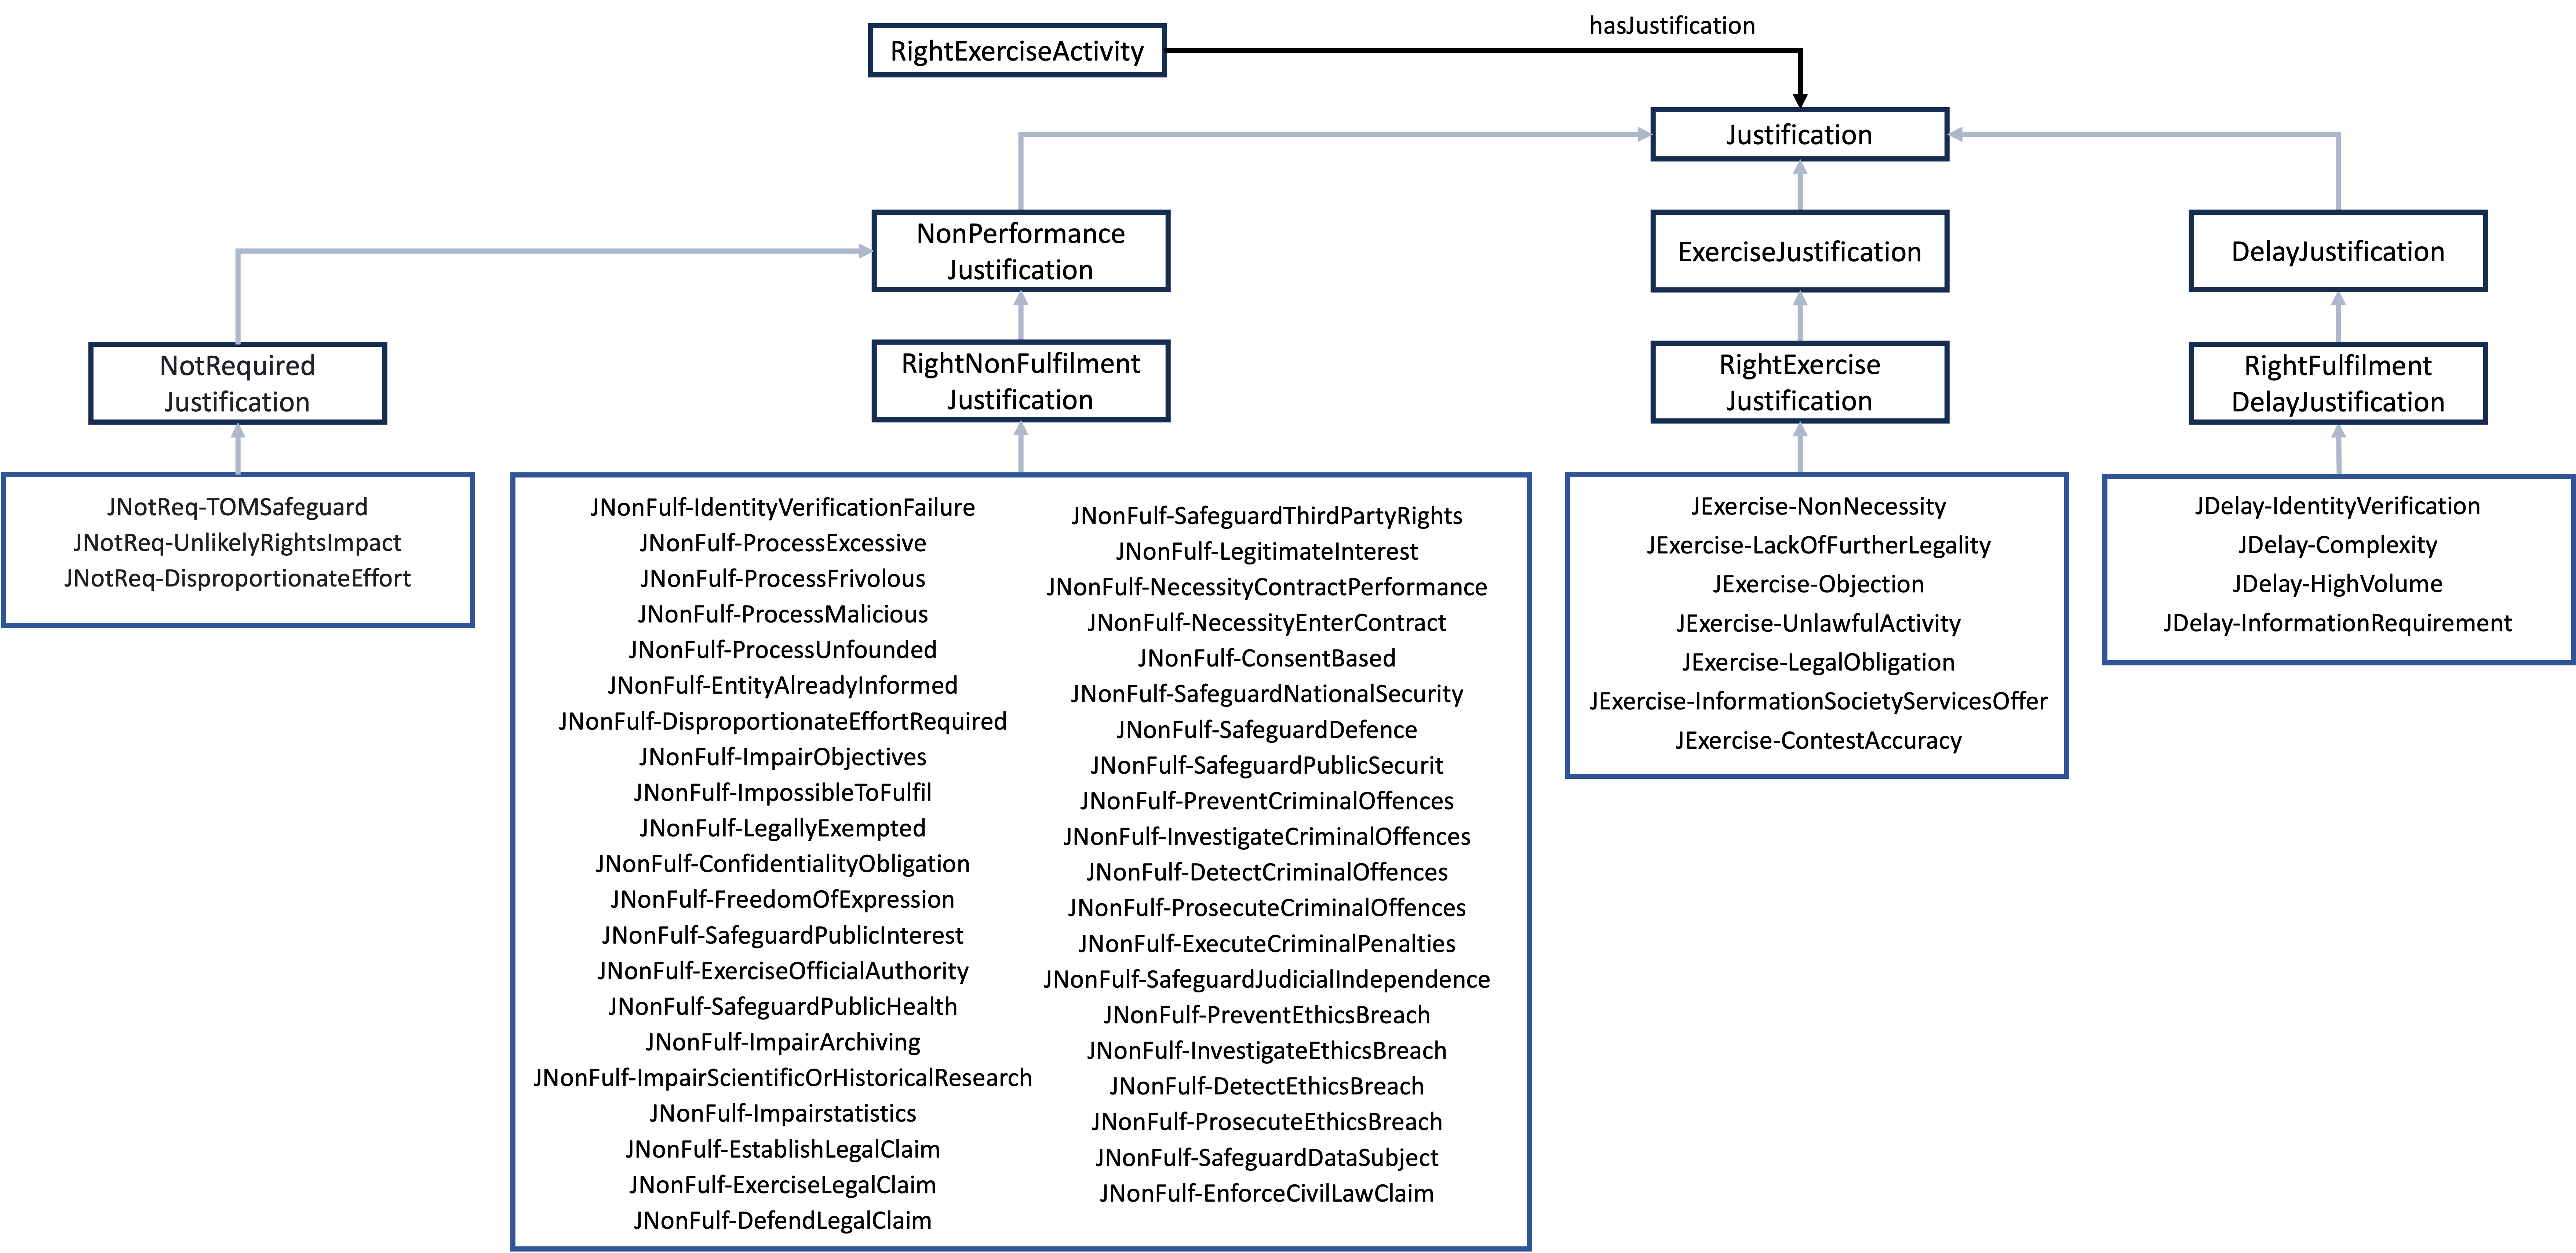
\includegraphics[width=\linewidth]{figures/chapter-4/justifications.png}
    \caption[Justification concepts.]{Justification concepts for the non-fulfilment, delay of fulfilment and exercise of rights.}
    \label{fig:justifications}
\end{figure}

Additionally, to track the status of rights exercising activities, a set of request statuses are modelled in DPV, including \texttt{RequestAccepted} for a request being accepted towards fulfilment, \texttt{RequestRejected} for a request being rejected towards non-fulfilment or\linebreak \texttt{RequestRequiresAction} for a request requiring an action to be performed from another party, and the \texttt{isBefore} and \texttt{isAfter} concepts can be used to specify that a specific activity occurs before or after another activity.

While this modelling was inspired by the GDPR, the concepts are described in a jurisdiction-agnostic manner so that they can be used to tackle data protection regulations in different jurisdictions.
For GDPR-specific rights, the \texttt{DataSubjectRight} concept is extended in DPV-GDPR with the data subject rights described in GDPR's Articles 13 to 22, as well as the rights to withdraw consent and to lodge a complaint with a supervisory authority, described in Articles 7.3 and 77.
Moreover, notices for direct and indirect data collection, to fulfil the information requirements in Articles 13 and 14, for Subject Access Requests (SARs), described in Article 15, and for notifying recipients, necessary to fulfil the communication requirements of Articles 16, 17 and 18, are provided as GDPR-specific subclasses of \texttt{RightFulfilmentNotice}s.

An overview of the aforementioned requirements and the intended purpose for modelling these concepts is presented in the ORSD illustrated in Table~\ref{tab:rights_ORSD}.

% also with these questions(in the ORSD) can you link directly to gdpr articles or other literature of gdpr implementation that help indicate these are valid requirements?

\begin{table}[htbp]
\centering
\caption{ORSD of the proposed model to express rights-related activities.}
\label{tab:rights_ORSD}
\scriptsize
\resizebox{\textwidth}{!}{%
\begin{tabular}{| l | l | l | l  | l | l | l |l| }
\hline
\multicolumn{8}{|c|}{\cellcolor[HTML]{A0A0A0}\textbf{Vocabulary-based patterns for rights exercising activities}} \\ \hline
\multicolumn{8}{|c|}{\cellcolor[HTML]{EFEFEF}\textbf{1. Purpose}} \\ \hline
\multicolumn{8}{| p{12.0cm} |}{The purpose of this model is the expression of rights-related activities, in particular focusing on data subject rights, such as the ones described in GDPR's Chapter III.} \\ \hline
\multicolumn{8}{|c|}{\cellcolor[HTML]{EFEFEF}\textbf{2. Scope}} \\ \hline
\multicolumn{8}{| p{12.0cm} |}{The scope of this model is limited to the expression of information related to the various steps of exercising data subject rights. In particular, the introduced concepts serve one of these purposes: (i) indicate what rights exist, (ii) express where such rights can be exercised, and (iii) record information related to concrete instances of rights that are being or were exercised. } \\ \hline
\multicolumn{8}{|c|}{\cellcolor[HTML]{EFEFEF}\textbf{3. Implementation Language}} \\ \hline
\multicolumn{8}{| p{12.0cm} |}{RDF, RDFS} \\ \hline
\multicolumn{8}{|c|}{\cellcolor[HTML]{EFEFEF}\textbf{4. Intended End-Users}} \\ \hline
\multicolumn{8}{| p{12.0cm} |}{Developers of Web services and applications, including decentralised storage solutions, that handle personal data.} \\ \hline
\multicolumn{8}{|c|}{\cellcolor[HTML]{EFEFEF}\textbf{5. Intended Uses}} \\ \hline
\multicolumn{8}{| p{12.0cm} |}{
Use 1. Declaration of the existence of data subject rights when the usage and collection of personal data is performed by Web services providers and developers, including information on where they can be exercised. \newline
Use 2. Patterns for data subject rights that can be fulfilled. \newline
Use 3. Patterns for data subject rights that cannot be fulfilled, including justifications for non-fulfilment. \newline
Use 4. Fulfilment of data subject rights requests from specific data protection legislation, such as the GDPR.
 } \\ \hline
\multicolumn{8}{|c|}{\cellcolor[HTML]{EFEFEF}\textbf{6. Ontology Requirements}} \\ \hline
\multicolumn{8}{|c|}{\cellcolor[HTML]{EFEFEF}\textbf{a. Non-Functional Requirements}}    \\ \hline
\multicolumn{8}{| p{12.0cm} |}{
NFR 1. The concepts are either published online within DPVCG's outputs, following W3C's specification format, or are under discussion for being adopted by the same CG. } \\ \hline
\multicolumn{8}{|c|}{\cellcolor[HTML]{EFEFEF}\textbf{b. Functional  Requirements: Groups of Competency Questions}}  \\ \hline
\multicolumn{5}{|c|}{\cellcolor[HTML]{EFEFEF}CQRG1. Related to data subject rights} & \multicolumn{3}{|c|}{\cellcolor[HTML]{EFEFEF}CQRG2. Related to GDPR} \\ \hline
\multicolumn{5}{ | m{7cm} |}{
CQR1. What rights are applicable in a given context? \newline
CQR2. Where can the right be exercised? \newline
CQR3. How can the right be exercised? \newline
CQR4. What data is necessary to implement the right? \newline 
CQR5. Which entity implements the right? \newline 
CQR6. Which entity exercised the right? \newline 
CQR7. When is the exercising activity occurring? \newline 
CQR8. What is the status of the right request? } & 
\multicolumn{3}{ m{5cm} |}{
CQR9. Which data subject rights are applicable according to the legal basis used by the data controller? \newline
CQR10. Which provenance metadata must controllers provide when replying to data subject rights requests? \newline 
CQR11. Which justification can be provided to not fulfil, delay or exercise a request?
}\\ \hline
\end{tabular}}
\vspace{-0.1in}
\end{table}

\subsection{Vocabulary-based patterns for rights exercising activities}
\label{sec:rights_patterns}

This Section outlines the usage of DPV for the expression of rights exercising activities, specifically related to the data subject rights described in GDPR's Chapter III.
Accordingly, the \textit{``controller shall take appropriate measures to provide any information referred to in Articles 13 and 14 and any communication under Articles 15 to 22 [...] to the data subject in a concise, transparent, intelligible and easily accessible form''} and if \textit{``the data subject makes the request by electronic form means, the information shall be provided by electronic means where possible, unless otherwise requested by the data subject''} \citeyearpar{noauthor_regulation_2016}.
Consequently, in this Thesis, personal data processing-related vocabularies such as DPV, and other semantic metadata vocabularies such as DCMI Metadata Terms and DCAT, are used for the establishment of structured notices and records of activities, which promote the fulfilment of the transparency and machine-readability requirements previously described.
Additionally, by storing such information in decentralised personal datastores, the accessibility requirement can also be satisfied.

Listing~\ref{list:applicable_rights} provides an example of a personal data handling activity, which can be used to express information regarding the what, how, where, who, and why personal data is being processed, as well as what rights exist.
The example provides information regarding the type of personal data, \texttt{pd:EmailAddress}, being processed by the \texttt{ex:DataController}, the purpose and legal basis used for the processing to occur, \texttt{dpv:ServiceProvision} and \texttt{eu-gdpr:A6-1-a}, and the applicable GDPR data subject rights.
This pattern can be followed by data controllers to express which rights are applicable, including rights beyond the ones in the GDPR, e.g., EU's fundamental rights and the rights depicted in other EU regulations or in other jurisdictions.

\begin{listing}[htp]
\caption[Personal data handling activity with applicable rights.]{Personal data handling activity example which includes information regarding the applicable rights.}
\label{list:applicable_rights}
\begin{minted}{turtle}
ex:ProcessEmailForServiceProvision a dpv:PersonalDataHandling ;
    dpv:hasDataController ex:DataController ;
    dpv:hasPersonalData pd:EmailAddress ;
    dpv:hasProcessing dpv:Collect, dpv:Use ;
    dpv:hasPurpose dpv:ServiceProvision ;
    dpv:hasLegalBasis eu-gdpr:A6-1-a ;
    dpv:hasRight eu-gdpr:A7-3, eu-gdpr:A13, eu-gdpr:A14, eu-gdpr:A15, eu-gdpr:A16, eu-gdpr:A17, eu-gdpr:A18, eu-gdpr:A20, eu-gdpr:A22, eu-gdpr:A77 .
ex:DataController a dpv:DataController .
\end{minted}
\end{listing}

Moreover, such declarations of applicable rights should include a notice of where they can be exercised.
Thus, as described in the previous Section, DPV’s \texttt{isExercisedAt} property should be used to connect rights with information on where to exercise it.
Such information should be provided through a \texttt{RightExerciseNotice}, along with other rights exercising metadata.

Listing~\ref{list:exercise_point} provides a notice with information on where to exercise the GDPR's right of access related to personal data being processed by the \texttt{ex:DataController}.
This notice uses the \texttt{dpv:hasRight} property to indicate which rights can be exercised, beyond the already mentioned access right, and the \texttt{foaf:page} property to express the precise Web page where the right can be exercised.
Additionally, DPV's \texttt{hasDataController} and\linebreak \texttt{isImplementedByEntity} properties are used to define who is the controller responsible for the personal data being processed and who is the entity implementing the service/platform where the rights are exercised -- in most cases this entity will probably coincide with the data controller, however, for transparency and accountability purposes, it is reasonable to express both terms.
Other entity-related properties can also be used to personalise the notice, e.g., if a notice is personalised for a specific data subject, then \texttt{dpv:hasDataSubject} can be used to connect the notice with the individual data subject. 
Furthermore, personal data handling instances can also be used to express `data processing bundles' that need to be provided in order to fulfil the data subjects' rights.
As previously mentioned, this can be done using DPV's taxonomies of purposes, personal data categories, processing operations, etc, e.g., in Listing~\ref{list:exercise_point}, an account identifier is required by the data controller for identity verification purposes in order to fulfil the data subject's rights described in GDPR's Articles 7.3, 15, 16, 17 and 20.
Other information might be needed to be communicated to the user, for instance, information on payments as Article 12.5(a) states that a fee \textit{``taking into account the administrative costs of providing the information or communication or taking the action requested''} might be requested by the data controller in case the data subject's request is unfounded, excessive or repetitive.
Such information can also be expressed in personal data handling instances including ODRL policies with duties constrained with an \texttt{odrl:payAmount} left operand.
% need to be provided / are being provided

\begin{listing}[htp]
\caption[GDPR Article 15's right of access exercise notice.]{GDPR Article 15's right of access exercise notice, including information on where to exercise the right and on necessary data to fulfil the right.}
\label{list:exercise_point}
\begin{minted}{turtle}
ex:RightToAccess a eu-gdpr:A15 ;
    dpv:isExercisedAt ex:RightExercisePoint .

ex:RightExercisePoint a dpv:RightExerciseNotice ;
    dpv:hasRight eu-gdpr:A7-3, eu-gdpr:A15, eu-gdpr:A16, eu-gdpr:A17, eu-gdpr:A20 ;
    dpv:hasDataController ex:DataController ;
    dpv:isImplementedByEntity ex:DataController ;
    foaf:page <https://example.com/DataController/RightExercisePoint> ;
    dpv:hasPersonalDataHandling [ 
        a dpv:PersonalDataHandling ;
        dpv:hasPurpose dpv:IdentityVerification ;
        dpv:hasPersonalData pd:AccountIdentifier ;
        dpv:hasProcessing dpv:Collect, dpv:Store ;
        dpv:hasRecipientDataController ex:DataController ] .
\end{minted}
\end{listing}

In addition to notices expressing what rights are applicable and where they can be exercised, provenance metadata must be kept when actual instances of the rights are exercised, throughout the whole process, from initiating a request to rejecting or fulfilling it.
As such, DPV's \texttt{RightExerciseActivity} can be used in conjunction with the W3C's PROV-O recommendation~\citep{lebo_prov-o_2013} to track the provenance of a right exercising activity instance.
Using this standard, provenance information, regarding the entities whom the request is associated with, i.e., \texttt{prov:wasAssociatedWith}, or what data/notice was generated, i.e., \texttt{prov:generated}, by the right exercise activity, can be represented.
\texttt{prov:actedOnBehalfOf} can also be used to represent delegation or representation, for instance when a parent exercises a right on behalf of its child.
Temporal information, descriptions and identifiers of the activities and their creators/publishers can be recorded using DCMI Metadata Terms.
Connections to the previous or following activities can be done using the \texttt{dpv:isAfter} and \texttt{dpv:isBefore} concepts, respectively.
Moreover, to track the status of a right exercising activity, DPV's taxonomy of request statuses concepts can be used.

Figure~\ref{fig:request_status} illustrates the sequence in which these concepts occur.
Once the request is initiated, it should be then acknowledged by the entity implementing it and either accepted towards fulfilment or rejected towards non-fulfilment.
Additionally, after being rejected, the entity fulfilling the request can also require further action from the requester (e.g., request additional data to be able to fulfil the request), which can delay the acceptance or rejection of the request, and after the required action is performed, the request can either be accepted towards fulfilment or get rejected again towards non-fulfilment or towards asking again for further action.

% perhaps formalise the semantics a bit more using uml state machine notation?
\begin{figure}[htp]
    \centering
    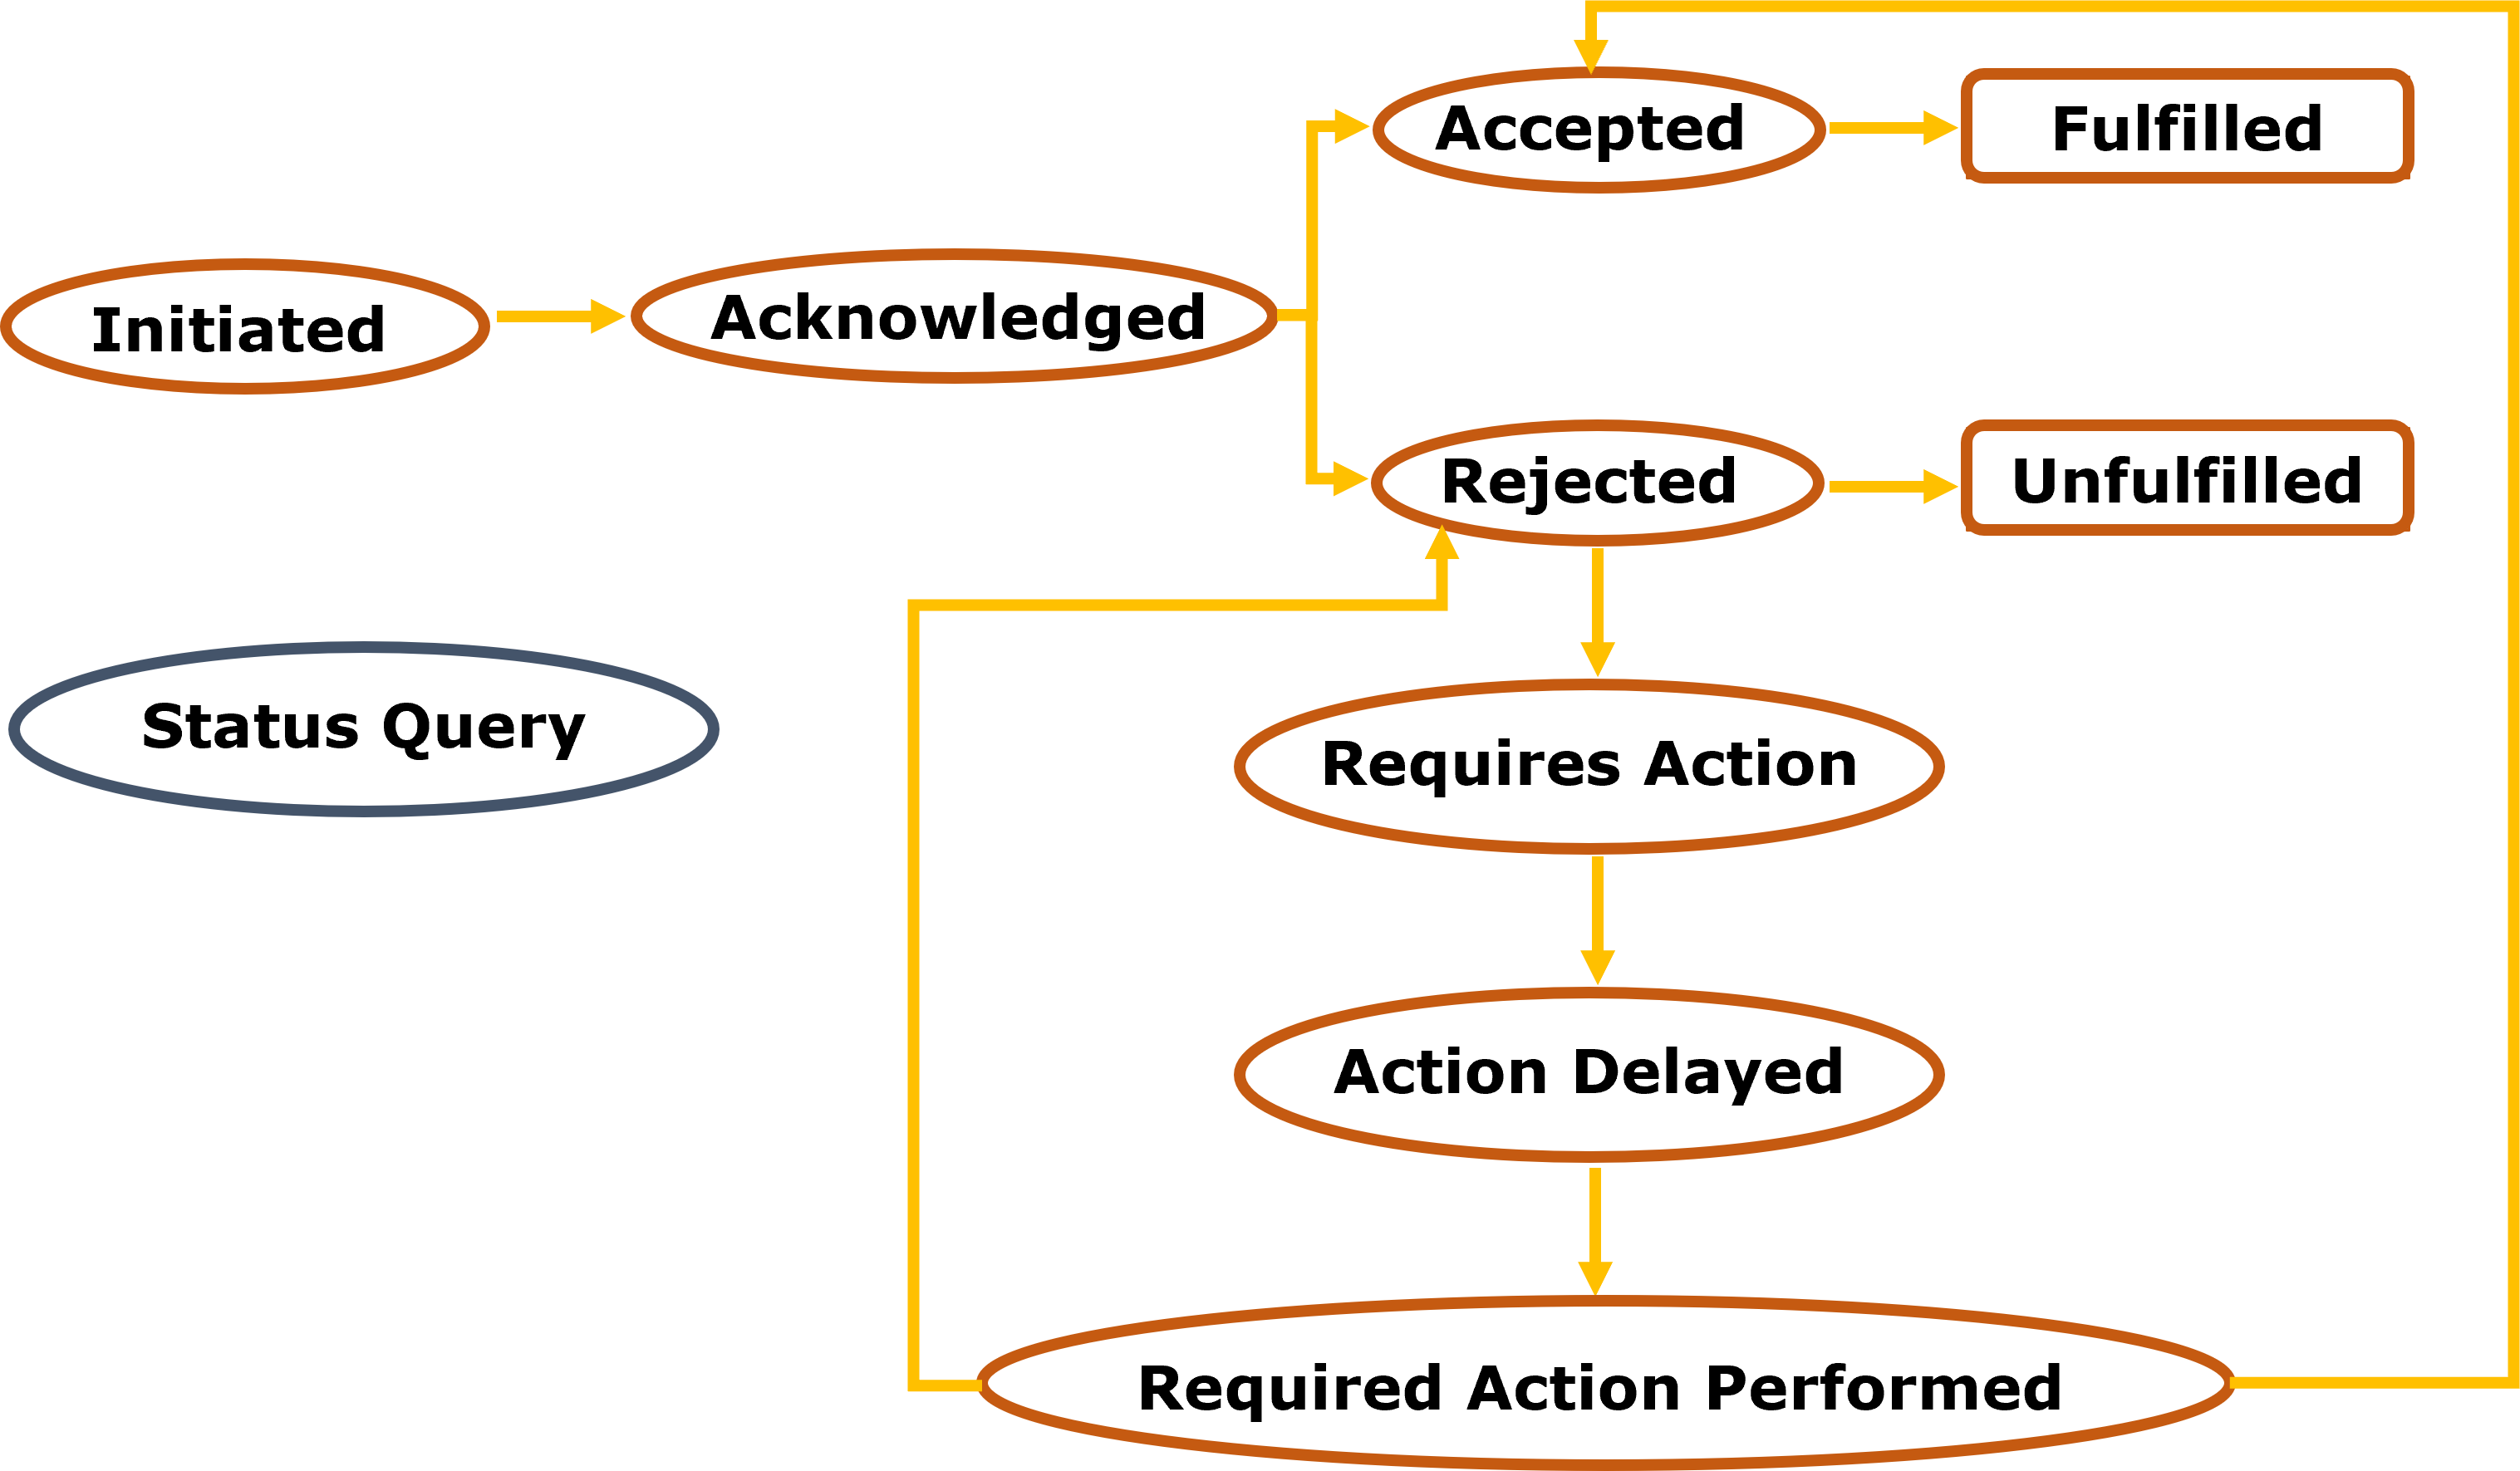
\includegraphics[width=0.8\linewidth]{figures/chapter-4/request-status.png}
    \caption{DPV's concepts to model the status of a request.}
    \label{fig:request_status}
\end{figure}

Listing~\ref{list:request_acknowledgment} illustrates a record of the right exercising activities related to a GDPR right of access request and acknowledgement of said request.
The activity associated with the start of the request has the status \texttt{dpv:RequestInitiated}, the data subject is identified using the \texttt{dpv:hasDataSubject} and the recipient of the request, a data controller, using the \texttt{dpv:hasRecipientDataController}.
Furthermore, a personal data handling instance can be used to express what personal data needs to be processed for the fulfilment of the right and DPV's \texttt{hasScope} to specify the scope of the request, e.g., the data subject only wants to access data processed for service provision purposes or only data processed during 2022.
Following the start of the request, the controller acknowledges the request, a right exercising activity which has \texttt{dpv:RequestAcknowledged} status and the recipient is the data subject that initiated the request.

\begin{listing}[htp]
\caption{Record of GDPR right of access request and acknowledgement activities.}
\label{list:request_acknowledgment}
\begin{minted}{turtle}
ex:DataSubject a dpv:DataSubject .
ex:DataSubjectUsername a pd:AccountIdentifier ;
    dpv:hasDataSubject ex:DataSubject .

ex:SARequest a dpv:RightExerciseActivity, prov:Activity ;
    dcterms:description "Data Subject makes a GDPR right of access request" ;
    dpv:hasRight eu-gdpr:A15 ;
    dpv:isExercisedAt ex:RightExercisePoint ;
    prov:wasAssociatedWith ex:DataSubject ;
    dpv:hasDataSubject ex:DataSubject ;
    dpv:hasRecipientDataController ex:DataController ;
    dcterms:date "2023-11-02T11:08:05"^^xsd:dateTime ;
    dpv:hasStatus dpv:RequestInitiated ;
    dpv:hasPersonalDataHandling [
        a dpv:PersonalDataHandling ;
        dpv:hasPurpose dpv:IdentityVerification ;
        dpv:hasPersonalData ex:DataSubjectUsername ;
        dpv:hasProcessing dpv:Collect, dpv:Store ] ;
    dpv:hasScope [
        dpv:hasPurpose dpv:ServiceProvision ;
        dpv:hasDuration [
            time:hasBeginning "2022-01-01T00:00:00"^^xsd:dateTime ;
            time:hasEnd "2022-12-31T23:59:59"^^xsd:dateTime ] ] .

ex:SARAcknowledged a dpv:RightExerciseActivity, prov:Activity ;
    dcterms:description "Data controller acknowledges the request" ;
    dcterms:date "2023-11-02T15:55:10"^^xsd:dateTime ;
    prov:wasAssociatedWith ex:DataController ;
    dpv:hasRecipient ex:DataSubjectUsername ;
    dpv:hasStatus dpv:RequestAcknowledged ;
    dpv:isAfter ex:SARequest .
\end{minted}
\end{listing}

Listing~\ref{list:further_action} illustrates the follow-up to Listing~\ref{list:request_acknowledgment} -- the request was rejected\linebreak due to the data controller not being able to identify the data subject,\linebreak \texttt{JNonFulf-IdentityVerificationFailure}.
Table~\ref{tab:justifications} contains the list of modelled right non-fulfilment justifications and their labels, which can be used by controllers for the purpose of justifying such requests.
As such the data controller requires further information from the data subject to be able to proceed with the request.
Such right exercise activity is identified with the \texttt{dpv:RequestRequiresAction} status and contains a personal data handling activity instance expressing the information that the data subject needs to provide for the right exercise to continue.
Afterwards, a right exercise activity associated with the data subject and with a \texttt{dpv:RequestRequiredActionPerformed} status is recorded with the information that the data subject provided.

\begin{listing}[htp]
\caption[Record requesting further information to fulfil SAR.]{Record of data controller requesting further information to fulfil the data subject's SAR and of the data subject providing the controller with said information.}
\label{list:further_action}
\begin{minted}{turtle}
ex:SARRejected a dpv:RightExerciseActivity, prov:Activity;
    dcterms:description "Data controller rejects the request" ;
    dcterms:date "2023-11-02T15:57:31"^^xsd:dateTime ;
    prov:wasAssociatedWith ex:DataController ;
    dpv:hasRecipient ex:DataSubjectUsername ;
    dpv:hasStatus dpv:RequestRejected ;
    dpv:hasJustification justif:JNonFulf-IdentityVerificationFailure ;
    dpv:isAfter ex:SARAcknowledged .

ex:SARRequiresAction a dpv:RightExerciseActivity, prov:Activity ;
    dcterms:description "Data controller requires further actions" ;
    dcterms:date "2023-11-02T16:09:21"^^xsd:dateTime ;
    prov:wasAssociatedWith ex:DataController ;
    dpv:hasRecipient ex:DataSubjectUsername ;
    dpv:hasStatus dpv:RequestRequiresAction ;
    dpv:hasJustification justif:JNonFulf-IdentityVerificationFailure ;
    dpv:hasPersonalDataHandling [
        dpv:hasPersonalData pd:OfficialID ;
        dpv:hasProcessing dpv:MakeAvailable ;
        dpv:hasPurpose dpv:IdentityVerification ;
        dpv:hasRecipientDataController ex:DataController ;
        dpv:isImplementedByEntity ex:DataSubjectUsername ] ;
    dpv:isAfter ex:SARRejected .

ex:DataSubjectOfficialID a pd:OfficialID ;
    dpv:hasDataSubject ex:DataSubject .

ex:SARActionPerformed a dpv:RightExerciseActivity, prov:Activity ;
    dcterms:description "Data Subject provides required information" ;
    dcterms:date "2023-11-02T17:20:42"^^xsd:dateTime ;
    prov:wasAssociatedWith ex:DataSubject ;
    dpv:hasStatus dpv:RequestRequiredActionPerformed ;
    dpv:hasPersonalDataHandling [
        dpv:hasPersonalData ex:DataSubjectOfficialID ;
        dpv:hasProcessing dpv:MakeAvailable ;
        dpv:hasPurpose dpv:IdentityVerification ;
        dpv:hasRecipientDataController ex:DataController ;
        dpv:isImplementedByEntity ex:DataSubjectUsername ] ;
    dpv:isAfter ex:SARRequiresAction .
\end{minted}
\end{listing}

% rights non-fulfilment justifications issue: https://github.com/w3c/dpv/issues/63 & meeting minutes:https://www.w3.org/2022/10/19-dpvcg-minutes.html
\begin{landscape}
\begin{table}
    \centering
    \caption{Justifications for non-fulfilment of GDPR's data subject rights.}
    \label{tab:justifications}
    \resizebox{\textwidth}{!}{%
    \begin{tabular}{c|l|c}
        \textbf{Term} & \textbf{Label} & \multicolumn{1}{c}{\begin{tabular}[c]{@{}c@{}} \textbf{GDPR} \\ \textbf{Article(s)} \end{tabular}} \\
        \hline\hline
        \texttt{JNonFulf-IdentityVerificationFailure} & \multicolumn{1}{l|}{\begin{tabular}[l]{@{}l@{}} Justification that the process could not be fulfilled or was not successful\\ because identity verification failed \end{tabular}} & 12.2 \\
        \hline
        \texttt{JNonFulf-ProcessExcessive} & Request was excessive in scope & 12.5 \\
        \hline
        \texttt{JNonFulf-ProcessFrivolous} & Request was frivolous in scope & 12.5 \\
        \hline
        \texttt{JNonFulf-ProcessMalicious} & Request was malicious in scope & 12.5 \\
        \hline
        \texttt{JNonFulf-ProcessUnfounded} & Request was unfounded in scope & 12.5 \\
         \hline
        \texttt{JNonFulf-EntityAlreadyInformed} & \multicolumn{1}{l|}{\begin{tabular}[l]{@{}l@{}} Data subject already has been provided with this information \end{tabular}} & 13.4, 14.5(a) \\
         \hline
        \texttt{JNonFulf-ImpairObjectives} & Fulfilment would cause impairment to processing & 14.5(b) \\
        \hline     
        \texttt{JNonFulf-DisproportionateEffortRequired} & Fulfilment would require extraordinary effort & 14.5(b), 19 \\
         \hline
        \texttt{JNonFulf-ImpossibleToFulfil} & Fulfilment would be impossible & 14.5(b), 19 \\
         \hline
        \texttt{JNonFulf-LegallyExempted} & \multicolumn{1}{l|}{\begin{tabular}[l]{@{}l@{}} Fulfilment not needed as it falls under legal exemption \end{tabular}} & \multicolumn{1}{l}{\begin{tabular}[l]{@{}l@{}} 14.5(c), 17.3(b),\\ 22.2(b) \end{tabular}} \\
         \hline
        \texttt{JNonFulf-ConfidentialityObligation} & \multicolumn{1}{l|}{\begin{tabular}[l]{@{}l@{}} Fulfilment would compromise existing confidentiality obligations \end{tabular}} & 14.5(d) \\
        \hline
        \texttt{JNonFulf-FreedomOfExpression} & \multicolumn{1}{l|}{\begin{tabular}[l]{@{}l@{}} Fulfilment would interfere with the right of freedom of expression\\ and information of others \end{tabular}} & 17.3(a) \\
         \hline
        \texttt{JNonFulf-SafeguardPublicInterest} & \multicolumn{1}{l|}{\begin{tabular}[l]{@{}l@{}} Fulfilment would interfere with necessary tasks carried out for public\\ interest \end{tabular}} & \multicolumn{1}{l}{\begin{tabular}[l]{@{}l@{}} 17.3(b), 21.6,\\ 23.1(e) \end{tabular}} \\
         \hline
         \texttt{JNonFulf-ExerciseOfficialAuthority} & \multicolumn{1}{l|}{\begin{tabular}[l]{@{}l@{}} Fulfilment would interfere with the exercise of official authorities \end{tabular}} & \multicolumn{1}{l}{\begin{tabular}[l]{@{}l@{}} 17.3(b), 20.3,\\ 23.1(h) \end{tabular}} \\
         \hline
         \texttt{JNonFulf-SafeguardPublicHealth} & \multicolumn{1}{l|}{\begin{tabular}[l]{@{}l@{}} Fulfilment would interfere with necessary tasks carried out for public\\ health reasons \end{tabular}} & 17.3(c) \\
         \hline
        \texttt{JNonFulf-ImpairArchiving} & \multicolumn{1}{l|}{\begin{tabular}[l]{@{}l@{}} Fulfilment would compromise or hinder archiving purposes \end{tabular}} & 17.3(d) \\
        \hline
        \texttt{JNonFulf-ImpairScientificOrHistoricalResearch} & \multicolumn{1}{l|}{\begin{tabular}[l]{@{}l@{}} Fulfilment would impair scientific or historical research \end{tabular}} & 17.3(d) \\
        \hline
        \texttt{JNonFulf-ImpairStatistics} & \multicolumn{1}{l|}{\begin{tabular}[l]{@{}l@{}} Fulfilment would interfere with official statistics \end{tabular}} & 17.3(d) \\
        \hline
        \texttt{JNonFulf-EstablishLegalClaim} & \multicolumn{1}{l|}{\begin{tabular}[l]{@{}l@{}} Fulfilment would interfere with the establishment of legal claims \end{tabular}} & 17.3(e), 21.1 \\
        \hline
        \texttt{JNonFulf-ExerciseLegalClaim} & \multicolumn{1}{l|}{\begin{tabular}[l]{@{}l@{}} Fulfilment would interfere with the exercise of legal claims \end{tabular}} & 17.3(e), 21.1 \\
        \hline
        \texttt{JNonFulf-DefendLegalClaim} & \multicolumn{1}{l|}{\begin{tabular}[l]{@{}l@{}} Fulfilment would interfere with the defence of legal claims \end{tabular}} & 17.3(e), 21.1 \\
        \hline
        \texttt{JNonFulf-SafeguardThirdPartyRights} & \multicolumn{1}{l|}{\begin{tabular}[l]{@{}l@{}} Fulfilment would adversely affect the rights of other data subjects or third\\ parties \end{tabular}} & 20.4, 23.1(i) \\
         \hline
         \texttt{JNonFulf-LegitimateInterest} & \multicolumn{1}{l|}{\begin{tabular}[l]{@{}l@{}} Fulfilment would interfere with the legitimate interest of the controller\\ which overrides the interests or rights of the data subject \end{tabular}} & 21.1 \\
         \hline
        \texttt{JNonFulf-NecessityContractPerformance} & \multicolumn{1}{l|}{\begin{tabular}[l]{@{}l@{}} Fulfilment would interfere with the performance of a contract \end{tabular}} & 22.2(a) \\
         \hline
        \texttt{JNonFulf-NecessityEnterContract} & \multicolumn{1}{l|}{\begin{tabular}[l]{@{}l@{}} Fulfilment would interfere with the necessity of entering into a contract \end{tabular}} & 22.2(a) \\
         \hline
        \texttt{JNonFulf-ConsentBased} & \multicolumn{1}{l|}{\begin{tabular}[l]{@{}l@{}} Fulfilment not necessary as processing is based on explicit consent \end{tabular}} & 22.2(c) \\
        \hline
        \texttt{JNonFulf-SafeguardNationalSecurity} & \multicolumn{1}{l|}{\begin{tabular}[l]{@{}l@{}} Fulfilment would pose a threat to safeguard national security \end{tabular}} & 23.1(a) \\
         \hline
        \texttt{JNonFulf-SafeguardDefence} & Fulfilment would pose a threat to safeguard defence & 23.1(b) \\
         \hline
        \texttt{JNonFulf-SafeguardPublicSecurity} & \multicolumn{1}{l|}{\begin{tabular}[l]{@{}l@{}} Fulfilment would pose a threat to safeguard public security \end{tabular}} & 23.1(c) \\
         \hline
        \texttt{JNonFulf-PreventCriminalOffences} & \multicolumn{1}{l|}{\begin{tabular}[l]{@{}l@{}} Fulfilment would interfere with the prevention of criminal offences \end{tabular}} & 23.1(d) \\
        \hline
        \texttt{JNonFulf-InvestigateCriminalOffences} & \multicolumn{1}{l|}{\begin{tabular}[l]{@{}l@{}} Fulfilment would interfere with the investigation of criminal offences \end{tabular}} & 23.1(d) \\
        \hline
        \texttt{JNonFulf-DetectCriminalOffences} & \multicolumn{1}{l|}{\begin{tabular}[l]{@{}l@{}} Fulfilment would interfere with the detection of criminal offences \end{tabular}} & 23.1(d) \\
        \hline
        \texttt{JNonFulf-ProsecuteCriminalOffences} & \multicolumn{1}{l|}{\begin{tabular}[l]{@{}l@{}} Fulfilment would interfere with the prosecution of criminal offences \end{tabular}} & 23.1(d) \\
        \hline
        \texttt{JNonFulf-ExecuteCriminalPenalties} & \multicolumn{1}{l|}{\begin{tabular}[l]{@{}l@{}} Fulfilment would interfere with the execution of criminal penalties \end{tabular}} & 23.1(d) \\
        \hline
        \texttt{JNonFulf-SafeguardJudicialIndependence} & \multicolumn{1}{l|}{\begin{tabular}[l]{@{}l@{}} Fulfilment would pose a threat to safeguard judicial independence or\\ proceedings \end{tabular}} & 23.1(f) \\
        \hline
        \texttt{JNonFulf-PreventEthicsBreach} & \multicolumn{1}{l|}{\begin{tabular}[l]{@{}l@{}} Fulfilment would interfere with the prevention of breaches of ethics for\\ regulated professions \end{tabular}} & 23.1(g) \\
        \hline
        \texttt{JNonFulf-InvestigateEthicsBreach} & \multicolumn{1}{l|}{\begin{tabular}[l]{@{}l@{}} Fulfilment would interfere with the investigation of breaches of ethics for\\ regulated professions \end{tabular}} & 23.1(g) \\
        \hline
        \texttt{JNonFulf-DetectEthicsBreach} & \multicolumn{1}{l|}{\begin{tabular}[l]{@{}l@{}} Fulfilment would interfere with the detection of breaches of ethics for\\ regulated professions \end{tabular}} & 23.1(g) \\
        \hline
        \texttt{JNonFulf-ProsecuteEthicsBreach} & \multicolumn{1}{l|}{\begin{tabular}[l]{@{}l@{}} Fulfilment would interfere with the prosecution of breaches of ethics for\\ regulated professions \end{tabular}} & 23.1(g) \\
        \hline
        \texttt{JNonFulf-SafeguardDataSubject} & \multicolumn{1}{l|}{\begin{tabular}[l]{@{}l@{}} Fulfilment would interfere with the protection of the data subject \end{tabular}} & 23.1(i) \\
         \hline
        \texttt{JNonFulf-EnforceCivilLawClaim} & Fulfilment would interfere with the enforcement of civil law claims & 23.1(j) \\
    \end{tabular}}
\end{table}
\end{landscape}
% Information is legally exempt from disclosure	- Documents that have personal data of the data subject exempt from disclosure in court proceedings apply in relation to a Subject Access Request, this applies to both legal advice and litigation privilege

Listing~\ref{list:sar_notice} illustrates the follow-up to Listing~\ref{list:further_action} -- the request was accepted and fulfilled by the data controller and as such the data controller provides the data subject with a notice of the fulfilment of GDPR's Art.15, modelled as a \texttt{eu-gdpr:SARNotice}, and a copy of the data whose access was requested, modelled as a \texttt{dcat:Dataset}.
Beyond temporal information and providing the location of the notice, a personal data handling instance can be used to provide additional information to the data subject -- in the case of this SAR notice, the data subject is also notified of the type of personal data being processed, the purpose for the processing, the time period when the data was processed and the additional data subject rights that can be exercised.

\begin{listing}[htp]
\caption[Record of the acceptance and fulfilment of a SAR request.]{Record of the acceptance and fulfilment of the request and respective \texttt{SARNotice}.}
\label{list:sar_notice}
\begin{minted}{turtle}
ex:SARAccepted a dpv:RightExerciseActivity, prov:Activity ;
    dcterms:description "Request accepted by data controller towards fulfilment" ;
    dcterms:date "2023-11-03T08:15:04"^^xsd:dateTime ;
    prov:wasAssociatedWith ex:DataController ;
    dpv:hasRecipient ex:DataSubjectUsername ;
    dpv:hasStatus dpv:RequestAccepted ;
    dpv:isAfter ex:SARActionPerformed .

ex:SARFulfilled a dpv:RightExerciseActivity, prov:Activity ;
    dcterms:description "Request fulfilled by data controller" ;
    dcterms:date "2023-11-03T08:37:25"^^xsd:dateTime ;
    prov:wasAssociatedWith ex:DataController ;
    dpv:hasRecipient ex:DataSubjectUsername ;
    dpv:hasStatus dpv:RequestFulfilled ;
    prov:generated ex:DataCopy, ex:SARNotice_Username ;
    dpv:isAfter ex:SARAccepted .

ex:SARNotice_Username a eu-gdpr:SARNotice ;
    dcterms:date "2023-11-03T08:31:51"^^xsd:dateTime ;
    foaf:page <https://example.com/DataController/SARNotice_Username> ;
    dpv:hasPersonalDataHandling [
        dpv:hasPersonalData pd:EmailAddress ;
        dpv:hasPurpose dpv:ServiceProvision ;
        dpv:hasDuration [
            time:hasBeginning "2022-01-01T00:00:00"^^xsd:dateTime ;
            time:hasEnd "2022-12-31T23:59:59"^^xsd:dateTime ] ;
        dpv:hasRight eu-gdpr:A16, eu-gdpr:A17, eu-gdpr:A18, eu-gdpr:A21, eu-gdpr:A77 ] .

ex:DataCopy a dcat:Dataset ;
    dcterms:format <https://www.iana.org/assignments/media-types/text/csv> ;
    dcterms:accessRights access-right:c_16ec ; # restricted access
    dcterms:issued "2023-11-03T08:35:42"^^xsd:dateTime ;
    dcterms:valid "2023-12-03T08:35:42"^^xsd:dateTime ;
    dcat:landingPage <https://example.com/Username/SAR_DataCopy> .
\end{minted}
\end{listing}

Moreover, DCAT \citep{albertoni_data_2020} can be used to model resources beyond notices, for instance, a copy of the personal data, in the case of a right of access request according to the GDPR, as in Listing~\ref{list:sar_notice}.
Information regarding the format, validity and dataset provision/download location can be attached to the dataset representation using the \texttt{dcterms:format}, \texttt{dcterms:valid} and \texttt{dcat:landingPage} properties, respectively.
Additionally, DCAT -- and also the Data on the Web Best Practices Recommendation~\citep{loscio_data_2017} -- promotes the usage of ODRL to express license and rights statements, by linking the dataset with an ODRL policy using the \texttt{odrl:hasPolicy} property, or the usage of DCMI Metadata Terms' \texttt{license}, \texttt{accessRights} or \texttt{rights} properties to link datasets with licenses, access rights statements or other types of rights statements, e.g., copyrights, respectively.
In the case of using the latter, controlled vocabularies such as COAR's Access Rights vocabulary~\citep{apollaro_controlled_2022}, used in Listing~\ref{list:sar_notice} to restrict access only to the data subject, or the Named Authority List of Access rights from the~\cite{publications_office_of_the_european_union_named_2023} can be used to express `high-level' access control statements, e.g., embargoed, restricted or open access.
As such, by using DCAT and a policy expression vocabulary, i.e., ODRL, the user can easily control the transition of a compliance log and respective metadata, as proposed in PLASMA, from being only accessible by the user to be accessible by external auditors.

In this Section, the GDPR's Right of Access is used as an example to showcase how to model notices and right exercising activities using DPV, DCMI Metadata Terms, PROV-O and DCAT.
However, a similar pattern can be followed by data controllers to fulfil the other rights as in most cases the only substantial change would be the notice concept that needs to be used for a particular right instance, e.g., \texttt{eu-gdpr:DirectDataCollectionNotice} for the right fulfilment notice related to GDPR's Article 13, \texttt{eu-gdpr:IndirectDataCollectionNotice} for the right fulfilment notice related to GDPR's Article 14 or \texttt{eu-gdpr:RightsRecipientsNotice} for the right fulfilment notice related to GDPR's Article 19.
Moreover, some GDPR rights, such as the right to erasure in Article 17 and the right to restriction of processing in Article 18, also require the data subject to provide a justification for their request to be fulfilled by the data controller.
As such, a collection of justifications for the exercise of data subject rights, extracted from the GDPR and illustrated in Table~\ref{tab:fulfil_justifications}, was also modelled (as subclasses of a high-level \texttt{RightExerciseJustification} concept). % and is already approved to be integrated into DPV-GDPR's outputs.


\begin{table}
    \centering
    \caption[Justifications for the exercise of GDPR's data subject rights]{Justifications for the exercise of GDPR's data subject rights.}
    \label{tab:fulfil_justifications}
    \resizebox{\textwidth}{!}{%
    \begin{tabular}{c|p{8.5cm}|c}
        \textbf{Term} & \textbf{Label} & \multicolumn{1}{c}{\begin{tabular}[c]{@{}c@{}} \textbf{GDPR} \\ \textbf{Article(s)} \end{tabular}} \\
        \hline\hline
        \texttt{JExercise-NonNecessity} & \multicolumn{1}{l|}{\begin{tabular}[l]{@{}l@{}} Processing no longer necessary for the \\specified purposes \end{tabular}} & \multicolumn{1}{l}{\begin{tabular}[l]{@{}l@{}} 17.1(a),\\ 18.1(c) \end{tabular}} \\
        \hline
        \texttt{JExercise-LackOfFurtherLegality} & \multicolumn{1}{l|}{\begin{tabular}[l]{@{}l@{}} Processing no longer necessary due to a lack of further\\ legality of the legal basis of specified context \end{tabular}} & 17.1(b) \\
        \hline
        \texttt{JExercise-Objection} & Data subject objected to the processing & \multicolumn{1}{l}{\begin{tabular}[l]{@{}l@{}} 17.1(c),\\ 18.1(d) \end{tabular}} \\
        \hline
        \texttt{JExercise-UnlawfulActivity} & Personal data unlawfully processed & \multicolumn{1}{l}{\begin{tabular}[l]{@{}l@{}} 17.1(d),\\ 18.1(b) \end{tabular}} \\
        \hline
        \texttt{JExercise-LegalObligation} & Compliance with a legal obligation & 17.1(e) \\
        \hline
        \texttt{JExercise-InformationSocietyServicesOffer} & \multicolumn{1}{l|}{\begin{tabular}[l]{@{}l@{}} Personal data collected in relation to the offer \\of information society services \end{tabular}} & 17.1(f) \\
        \hline
        \texttt{JExercise-ContestAccuracy} & \multicolumn{1}{l|}{\begin{tabular}[l]{@{}l@{}} Accuracy of personal data contested by the \\data subject \end{tabular}} & 18.1(a) \\
    \end{tabular}}
\end{table}

\subsection{Justifications publication and maintenance}
\label{sec:justifications_publication}

As discussed in the previous sections, most rights-related concepts were already proposed and are integrated into DPV and DPV-GDPR.
The justifications concepts have already been approved to be accepted, but are still to be published in DPVCG's outputs.
As such, the justifications vocabulary human-readable documentation and machine-readable file are available at \url{https://w3id.org/people/besteves/justifications} using content negotiation.
Once the justification terms are fully integrated into DPV, this documentation will be archived as the maintenance of the terms will be performed as part of the DPVCG's activities.

The HTML documentation includes a description of the defined terms, which was conducted and validated with domain experts\footnote{This validation was performed with legal and ontology engineering experts in the context of W3C's DPV community group.}, diagrams with graphical representations of the several taxonomies used in the vocabulary patterns specific in this section, and RDF examples that use the defined terms to express rights-related activities.
The vocabulary documentation also includes metadata, such as the identity of the creators and publishers of the ontology, the dates of creation and last modification or the version number.
The source code is hosted at \url{https://w3id.org/people/besteves/justifications/repo}, under the CC-BY-4.0 license.
The repository can also be used by implementers to suggest new inclusions to the vocabulary and to report bugs through GitHub Issues.

Additionally, an auxiliary webpage, openly available at \url{https://w3id.org/people/besteves/rights}, provides guidelines and further examples on how to use DPV and the developed \texttt{Justification} terms to model the vocabulary-based patterns for rights-related activities defined in this Section.
The source code is hosted at \url{https://w3id.org/people/besteves/rights/repo}, under the CC-BY-4.0 license.
\section{Ontology quality evaluation}
\label{sec:evaluation}

This Section describes the results of the ontologies quality evaluation, including the detection of common pitfalls with OOPS!\footnote{The OOPS! tool is available at \url{https://oops.linkeddata.es/} (accessed on 14 June 2023).}~\citep{poveda-villalon_oops_2014}, alignment with FAIR principles with FOOPS!\footnote{The FOOPS! tool is available at \url{https://w3id.org/foops} (accessed on 30 November 2023).}~\citep{garijo_foops_2021} and validation of competency questions with SPARQL queries~\citep{harris_sparql_2013}.

In terms of quality evaluation, the OOPS! tool was used to evaluate PLASMA and OAC in order to detect common errors in ontology development, such as missing domain or range properties or missing human-readable annotations.
Both evaluations did not detect any critical (issues affecting the ontology consistency, reasoning, or applicability) or important (issues not critical for ontology functionality but that should be corrected) pitfalls.
Furthermore, FOOPS! was used to evaluate the alignment of the developed vocabularies with the FAIR (Findable, Accessible, Interoperable and Reusable) principles.
Additionally, the vocabularies that were reused in this Section, e.g., DPV, ODRL, or ActivityStreams, were also evaluated with FOOPS! for comparison.
Table~\ref{tab:foops_evaluation} presents the results of this evaluation.

\begin{table}[htp]
    \centering
    \caption{Evaluation of the alignment of the developed and reused vocabularies with FAIR principles using FOOPS!.}
    \label{tab:foops_evaluation}
    \resizebox{\textwidth}{!}{%
    \begin{tabular}{c||c|c|c|c|c}
        \textbf{Ontology} & \textbf{FOOPS! score} & \textbf{Findable} & \textbf{Accessible} & \textbf{Interoperable} & \textbf{Reusable} \\
        \hline\hline
        OAC & 91\% & 8/9 & 2/3 & 3/3 & 8.83/9 \\
        \hline
        PLASMA & 91\% & 8/9 & 2/3 & 3/3 & 8.83/9 \\
        \hline 
        DPV & 64\% & 5.33/9 & 2/3 & 3/3 & 4.92/9 \\
        \hline 
        ODRL & 64\% & 4.5/9 & 3/3 & 3/3 & 4.75/9 \\
        \hline
        DCAT & 64\% & 4.33/9 & 3/3 & 3/3 & 5.14/9 \\
        \hline
        ACP & 52\% & 5.33/9 & 2/3 & 2/3 & 3.12/9 \\
        \hline
        ActivityStreams & 19\% & 2/9 & 1.5/3 & 0/3 & 1/9 \\
        \hline 
        ACL & 2\% & 0/9 & 0.5/3 & 0/3 & 0/9 \\
        \hline
        DCMI & 2\% & 0/9 & 0.5/3 & 0/3 & 0/9 \\
    \end{tabular}}
\end{table}

Both PLASMA and OAC obtained a good score in all FAIR aspects.
In terms of improvements, both vocabularies will be submitted to LOV (Linked Open Vocabularies), a public registry of ontologies that includes ontology metadata related to its terms and the creators/developers of the ontologies~\citep{dumontier_linked_2017}.
This will improve both the findability and the accessibility of the vocabularies.
Using Table~\ref{tab:foops_evaluation}, it can be observed that both PLASMA and OAC rate much higher than other reused ontologies in terms of findability and reusability as the used URIs and version URIs are persistent and resolvable, both include the recommended ontology and ontology terms metadata, a resolvable data usage license and provenance metadata.

Additionally, SPARQL queries are used to assess whether the developed models satisfy the competency questions, presented in Tables~\ref{tab:OAC_ORSD}, \ref{tab:plasma_orsd} and \ref{tab:rights_ORSD}, which were used to guide the development of the vocabularies in order to fulfil the identified requirements.

Table~\ref{tab:oac_cq_sparql} presents the SPARQL queries drafted to fulfil OAC's competency questions presented in Table~\ref{tab:OAC_ORSD}.
The presented work demonstrates that OAC satisfies the identified requirements of answering competency questions regarding the modelling of policies representing personal preferences, requests of data for particular purposes, and agreements of data access, including contextual information.
In particular, these competency questions showcase OAC's capabilities for allowing the definition of different user preferences as policies, the specification of permissions and prohibitions at an arbitrary level of granularity, the identification and resolution of conflicting policies, and the usage of legally-aligned concepts, while also supporting users with easy access to the policies used for granting/denying access to data for internal and/or external introspection, thus fulfilling OAC's requirements outlined in Section~\ref{sec:oac_requirements}.

\begin{table}[htp]
    \centering
    \caption{Validation of OAC's competency questions with SPARQL queries.}
    \label{tab:oac_cq_sparql}
    \footnotesize
    \begin{tabular}{c||l}
        \textbf{CQO*} & \textbf{SPARQL query} \\
        \hline\hline
        CQO1 & \begin{lstlisting}[numbers=none]
SELECT ?policy WHERE {
    ?policy_uri a ?policy . 
    ?policy_uri odrl:uid ?policy_id . } \end{lstlisting} \\
        \hline
        CQO2 & \begin{lstlisting}[numbers=none]
SELECT ?action WHERE {
    ?policy_uri a ?policy . ?policy_uri odrl:uid ?policy_id . 
    ?policy_uri odrl:permission|odrl:prohibition ?rule .
    ?rule odrl:action ?action . } \end{lstlisting} \\
        \hline
        CQO3 & \begin{lstlisting}[numbers=none]
SELECT ?data WHERE {
    ?policy_uri a ?policy . ?policy_uri odrl:uid ?policy_id . 
    ?policy_uri odrl:permission|odrl:prohibition ?rule .
    ?rule odrl:target ?data . } \end{lstlisting} \\
        \hline
        CQO4 & \begin{lstlisting}[numbers=none]
SELECT ?constraint WHERE {
    ?policy_uri a ?policy . ?policy_uri odrl:uid ?policy_id . 
    ?policy_uri odrl:permission ?rule .
    ?rule odrl:constraint ?constraint . } \end{lstlisting} \\
        \hline
        CQO5 & \begin{lstlisting}[numbers=none]
SELECT ?assigner ?assignee WHERE {
    ?policy_uri a ?policy . ?policy_uri odrl:uid ?policy_id . 
    ?policy_uri odrl:permission|odrl:prohibition ?rule .
    OPTIONAL { ?rule odrl:assigner ?assigner } . 
    OPTIONAL { ?rule odrl:assignee ?assignee } . } \end{lstlisting} \\
        \hline
        CQO6 & \begin{lstlisting}[numbers=none]
SELECT ?conflict_term WHERE {
    ?policy_uri a ?policy . ?policy_uri odrl:uid ?policy_id . 
    ?policy_uri odrl:conflict ?conflict_term . } \end{lstlisting} \\
        \hline
        CQO7 & \begin{lstlisting}[numbers=none]
SELECT ?context WHERE {
    ?policy_uri a ?policy . ?policy_uri odrl:uid ?policy_id . 
    ?policy_uri odrl:permission|odrl:prohibition ?rule .
    ?rule dpv:hasContext ?context . } \end{lstlisting} \\
        \hline
        CQO8 & \begin{lstlisting}[numbers=none]
SELECT ?legal_basis WHERE {
    ?policy_uri a ?policy . ?policy_uri odrl:uid ?policy_id . 
    ?policy_uri odrl:permission|odrl:prohibition ?rule .
    ?rule odrl:constraint ?constraint . 
    ?constraint odrl:leftOperand oac:LegalBasis .
    ?constraint odrl:rightOperand ?legal_basis . } \end{lstlisting} \\
        \hline
        CQO9 & \begin{lstlisting}[numbers=none]
SELECT ?entity ?address ?contact ?name WHERE {
    ?entity a oac:Entity . 
    ?entity dpv:hasAddress ?address . 
    ?entity dpv:hasContact ?contact .
    ?entity dpv:hasName ?name . } \end{lstlisting} \\
    \end{tabular}
\end{table}

Moreover, Table~\ref{tab:plasma_cq_concepts} lists concepts that can be used to answer the competency questions identified in PLASMA's ORSD, available in Table~\ref{tab:plasma_orsd}.
Listing~\ref{list:plasma_sparql_cq} illustrates how these concepts can be used in SPARQL queries to fulfil the \textit{``CQP1. Which Pod management data is stored in the Pod?''} and \textit{``CQP4. What policy describes the data access requirements of a certain app or service?''} competency questions.
A similar exercise can be done for the remaining competency questions.
The presented work demonstrates that PLASMA satisfies the requirements identified in Section~\ref{sec:plasma_requirements} of answering competency questions regarding the representation of information related to entities, infrastructure, and processes in Solid, the modelling of information related to legal roles in a jurisdiction-agnostic manner, and the definition of patterns to express apps and services policies, data usage logs and registries of data, schemas, apps, services, entities, and authorisations for convenient access to information.
The developed SHACL shapes also satisfy the identified requirements by ensuring compliance with PLASMA's conformance conditions described in detail in Section~\ref{sec:plasma_conformance}.

\begin{table}[htp]
    \centering
    \caption{Concepts in PLASMA and other vocabularies for answering competency questions defined in Table~\ref{tab:plasma_orsd}.}
    \label{tab:plasma_cq_concepts}
    \begin{tabular}{c||c}
        \textbf{CQP*} & \textbf{Concepts} \\
        \hline\hline
        CQP1 & \multicolumn{1}{c}{\begin{tabular}[c]{@{}c@{}} \texttt{PodManagementData}, \texttt{hasProvider}, \texttt{hasDeveloper}, \\ \texttt{implementedSolidPlatform}, \texttt{implementedSolidSpecification} \end{tabular}} \\
        \hline
        CQP2 & \texttt{DataLog}, \texttt{DataProvider}, \texttt{ResourceMetadata}, \texttt{DataAgreement} \\
        \hline
        CQP3 & \multicolumn{1}{c}{\begin{tabular}[c]{@{}c@{}} \texttt{Policy}, \texttt{Log}, \texttt{UserData}, \texttt{AppData}, \texttt{ServiceData}, \\ \texttt{PodManagementData}, \texttt{SchemaData} \end{tabular}} \\
        \hline
        CQP4 & \texttt{DataRequest}, \texttt{AppManifest}, \texttt{ServiceManifest} \\
        \hline
        CQP5 & \multicolumn{1}{c}{\begin{tabular}[c]{@{}c@{}} \texttt{InfrastructureProvider}, \texttt{PodProvider}, \texttt{PodDeveloper}, \\ \texttt{SolidPlatformProvider}, \texttt{SolidPlatformProvider} \end{tabular}} \\
        \hline
        CQP6 & \multicolumn{1}{c}{\begin{tabular}[c]{@{}c@{}} \texttt{DataLog}, \texttt{DataProvider}, \texttt{dcat:landingPage},\\ \texttt{dcat:distribution}, \texttt{dcat:accessURL}, \texttt{dcat:mediaType} \end{tabular}} \\
        \hline
        CQP7 & \multicolumn{1}{c}{\begin{tabular}[c]{@{}c@{}} \texttt{AccessControlRegistry}, \texttt{DataRegistry}, \texttt{DataSchemaRegistry},\\ \texttt{PolicyRegistry}, \texttt{AppRegistry}, \texttt{ServiceRegistry}, \texttt{UserRegistry} \end{tabular}} \\
        \hline
        CQP8 & \texttt{dpv:hasName}, \texttt{dpv:hasAddress}, \texttt{dpv:hasContact} \\
        \hline
        CQP9 & \multicolumn{1}{c}{\begin{tabular}[c]{@{}c@{}} \texttt{InfrastructureProvider}, \texttt{PodProvider}, \texttt{SolidPlatformProvider},\\ \texttt{dpv:Purpose}, \texttt{dpv:LegalBasis}, \texttt{Log}, \texttt{Notice} \end{tabular}} \\
    \end{tabular}
\end{table}

\begin{listing}[htp]
\caption{Example SPARQL queries to validate PLASMA's CQP1 and CQP4.}
\label{list:plasma_sparql_cq}
\begin{minted}{sparql}
SELECT ?provider ?developer ?platform ?spec WHERE {
    ?pod_data a plasma:PodManagementData . 
    ?pod_data plasma:hasProvider ?provider . 
    ?pod_data plasma:hasDeveloper ?developer .
    ?pod_data plasma:implementedSolidPlatform ?platform .
    ?pod_data plasma:implementedSolidSpecification ?spec . }

SELECT ?app ?appmanifest ?policy WHERE {
    ?app a plasma:App . 
    ?app plasma:hasAppManifest ?appmanifest . 
    ?appmanifest a plasma:AppManifest .
    ?appmanifest odrl:hasPolicy ?policy . }
\end{minted}
\end{listing}

Finally, Table~\ref{tab:rights_cq_sparql} presents the SPARQL queries drafted to fulfil the competency questions of the proposed model to express rights-related exercising activities presented in Table~\ref{tab:rights_ORSD}.
The presented work demonstrates that the developed model satisfies the requirements identified in Section~\ref{sec:rights_concepts} by answering competency questions regarding the modelling of the existence of data subject rights, how and where such rights can be exercised, what data is necessary to fulfil such rights and which entities are in charge of implementing and exercising it, how to keep records of said exercising activities, including timestamps, the status of the right request activity and other provenance metadata, which rights are applicable according to the legal basis used by the data controllers, and which justifications can be provided by them to not fulfil, delay or exercise a request.

\begin{table}[htp]
    \centering
    \caption{Validation of the competency questions of the proposed model to express rights-related exercising activities with SPARQL queries.}
    \label{tab:rights_cq_sparql}
    \footnotesize
    \begin{tabular}{c||l}
        \textbf{CQR*} & \textbf{SPARQL query} \\
        \hline\hline
        CQR1 & \begin{lstlisting}[numbers=none]
SELECT ?pdh ?right WHERE {
    ?pdh a dpv:PersonalDataHandling . ?pdh dpv:hasRight ?right . } \end{lstlisting} \\
        \hline
        CQR2 & \begin{lstlisting}[numbers=none]
SELECT ?right ?exercise_point WHERE {
    ?right a dpv:DataSubjectRight . 
    ?right dpv:isExercisedAt ?notice . 
    ?notice a dpv:RightExerciseNotice . 
    ?notice foaf:page ?exercise_point . } \end{lstlisting} \\
        \hline
        CQR3 & \begin{lstlisting}[numbers=none]
SELECT ?right ?notice WHERE {
    ?right a dpv:DataSubjectRight . 
    ?right dpv:isExercisedAt ?notice . 
    ?notice a dpv:RightExerciseNotice . } \end{lstlisting} \\
        \hline
        CQR4 & \begin{lstlisting}[numbers=none]
SELECT ?right ?necessary_data WHERE {
    ?right a dpv:DataSubjectRight . 
    ?right dpv:isExercisedAt ?notice . 
    ?notice a dpv:RightExerciseNotice .
    ?notice dpv:hasPersonalDataHandling ?necessary_data . } \end{lstlisting} \\
        \hline
        CQR5 & \begin{lstlisting}[numbers=none]
SELECT ?right ?implementer WHERE {
    ?right a dpv:DataSubjectRight . 
    ?right dpv:isExercisedAt ?notice . 
    ?notice a dpv:RightExerciseNotice .
    ?notice dpv:isImplementedByEntity ?implementer . } \end{lstlisting} \\
        \hline
        CQR6 & \begin{lstlisting}[numbers=none]
SELECT ?activity ?data_subject WHERE {
    ?activity a dpv:RightExerciseActivity .
    ?activity dpv:hasStatus dpv:RequestInitiated . 
    ?activity dpv:hasDataSubject ?data_subject . } \end{lstlisting} \\
        \hline
        CQR7 & \begin{lstlisting}[numbers=none]
SELECT ?activity ?date WHERE {
    ?activity a dpv:RightExerciseActivity . 
    ?activity dcterms:date ?date . } \end{lstlisting} \\
        \hline
        CQR8 & \begin{lstlisting}[numbers=none]
SELECT ?activity ?status WHERE {
    ?activity a dpv:RightExerciseActivity . 
    ?activity dpv:hasStatus ?status . } \end{lstlisting} \\
        \hline
        CQR9 & \begin{lstlisting}[numbers=none]
SELECT ?pdh ?legal_basis ?right WHERE {
    ?pdh a dpv:PersonalDataHandling . 
    ?pdh dpv:hasRight ?right . ?pdh dpv:hasLegalBasis ?legal_basis . } \end{lstlisting} \\
        \hline
        CQR10 & \begin{lstlisting}[numbers=none]
SELECT ?activity ?data_subject ?status ?date ?controller WHERE {
    ?activity a dpv:RightExerciseActivity . 
    ?activity dpv:hasStatus ?status . 
    ?activity dpv:hasDataSubject ?data_subject . 
    ?activity dcterms:date ?date . 
    ?activity prov:wasAssociatedWith ?controller . } \end{lstlisting} \\
        \hline
        CQR11 & \begin{lstlisting}[numbers=none]
SELECT ?activity ?justification WHERE {
    ?activity a dpv:RightExerciseActivity . 
    ?activity dpv:hasStatus dpv:RequestRejected . 
    ?activity dpv:hasJustification ?justification . } \end{lstlisting} \\
    \end{tabular}
\end{table}
\section{Alignment with the ISO/IEC 27560 standard}
\label{sec:iso_27560}

ISO and IEC are an international standardisation body with technical committees established to specify requirements and guidelines for particular technical activities.
The ISO/IEC 27560 standard on `Privacy technologies -- Consent record information structure' \textit{``specifies an interoperable, open and extensible information structure for recording PII principals' consent to PII processing''}~\citep{isoiec_jtc_1sc_27_isoiec_2023}.
It outlines requirements and recommendations regarding the utilisation of consent receipts and consent records related to the processing of personally identifiable information (PII).
Its objectives include facilitating (i) a consent record for data controllers, (ii) the exchange of consent details among information systems, and (iii) the management of the consent life cycle.
Figure~\ref{fig:iso_27560} showcases the information elements of the consent record and receipt structure specified in the ISO/IEC 27560 standard, including examples of what information should be entered in each field.

\begin{figure}[ht]
    \centering
    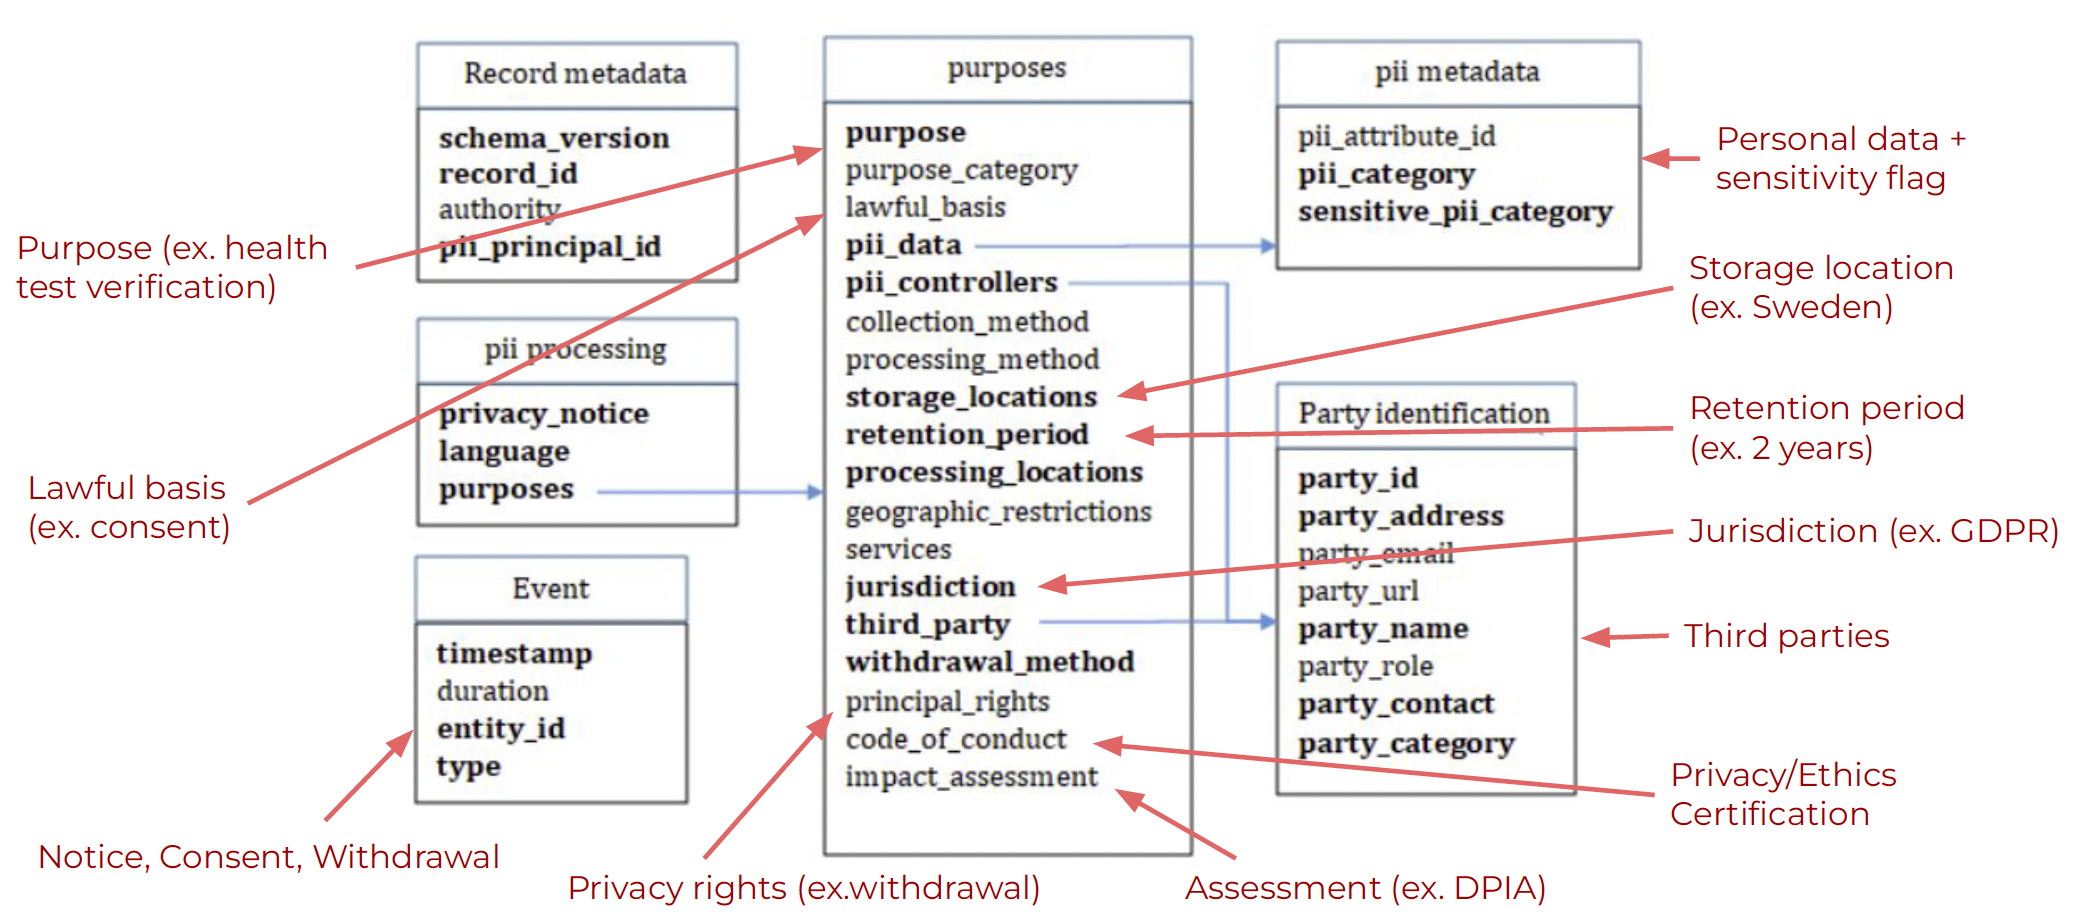
\includegraphics[width=1\linewidth]{figures//chapter-4/iso_27560.png}
    \caption{Elements of the ISO/IEC 27560 consent record and receipt structure~\citep{isoiec_jtc_1sc_27_isoiec_2023}.}
    \label{fig:iso_27560}
\end{figure}

Most of the fields illustrated in this Figure can be represented using the OAC-based data agreements proposed in Section~\ref{sec:oac}, as well as the existing ODRL and DPV specifications and the proposed work on PLASMA and the rights exercise extension described in Section~\ref{sec:plasma} and~\ref{sec:rights_exercising}.
The `record metadata' elements \textbf{record\_id}, \textbf{pii\_principal\_id}, and \textbf{authority} can be instantiated using the \texttt{odrl:uid}, the \texttt{dpv:hasDataSubject}, and the \texttt{dpv:hasAuthority} properties, and the `pii processing' terms \textbf{privacy\_notice}, and \textbf{language} with PLASMA's notice terms and \texttt{odrl:language} left operand.
Furthermore, the `Event' terms can be modelled using PLASMA and DPV's concepts to model notices, consent statuses, and logs of processing activities, and records of right exercise activities with the work proposed in Section~\ref{sec:rights_exercising}.
The `Party identification' elements can be modelled using the \texttt{oac:Entity} placeholder that should be set on agreement policies for assigners and assignees, as well as for constraints on which recipients can get access to the data, which can then be specifically defined with DPV's legal entity concepts as well as PLASMA entity terms to specify specific decentralised/Solid-related roles.
Contact-related information can also be modelled with DPV's \texttt{hasName}, \texttt{hasContact} and \texttt{hasAddress} properties.
Moreover, most `purposes' terms can already be modelled with existing and proposed work, such as the proposed OAC terms to restrict purposes, legal bases, data types, processing operations, including collection, or services, as well as existing ODRL temporal and spatial constraints, and DPV's concepts related rights, jurisdictions or impact assessments.
Additionally, DPV, and in particular its personal data extension, can be used to specify the categories of personal or sensitive personal data being used and specified in the standard as `pii metadata'.

As such, it is possible to check that the existing and proposed work is aligned with the ISO/IEC 27560 standard for consent records and hence can be used to fulfil almost all of the recommended elements.
Future work can be focused on providing machine-readable codes of conduct, and more comprehensive event specifications, e.g., data holders' permission terms proposed in the DGA.